\documentclass[12pt]{article}

\usepackage{amsmath}
\usepackage{amssymb}

\usepackage{graphicx}
\usepackage{float}
\begin{document}


\section{Outline/Goals}

\subsection{Goals}
\begin{itemize}
\item We have a complex dynamical system: high--dimensional, many scales (intrinsic and ambient), noisy (intrinsic and ambient), nonlinear (dynamics and observation function)
\item Our goal is to twofold
\begin{itemize}
	\item Recover the slow variables of the system
	\item Recover NIVs: the recovered slow variables should be in a ``canonical'' coordinate system, invariant to the obervation/measurement function and ambient noise
\end{itemize}
\item We do that through the solution of an eigenproblem of the kernel based on the Mahalanobis distance.
\item We want to study the effects of the dynamical system characteristics (scales, noises, nonlinearities) on the performance of NLICA and our ability to recover NIV. Furthermore, we want to layout the mathematical conditions reflecting this. 
\item When the mathematical conditions to recover NIV are not satisfied, we will look at constructing intermediate observers (i.e., histograms) to facilitate the recovery of NIVs through filtering out the fastest timescale by averaging/expected values. 
\end{itemize}


\subsection{Outline}

\begin{itemize}

\item Start with a simple example where we don't have NIV-- only do reduction; this emphasixes one of the effects of Mahalanobis-- filtering out the fast variables in order to recover {\em only} the slow variables. This is the 1d-1d orthoganol example, and the 1d-1d half moon example (and perhaps the chemical network example). In these cases, we do not care about estimating the covariances accurrately-- we only care about collapsing the fast direction(s). 
\item Another simple example for NIV-- the 2d example from Amit's NLICA paper. Here, the first thing we want to do is detemine how we can accurrately estimate the covariances when we have a time series, rather than short bursts. We will do this by comparing our estimates to the analytical covariance, and examining both the drift and curvature effects. 
\item An example that combines the first two examples: we now take Amit's NLICA example, and add fast noise on top of it. We now expect the covariance estimation to be ``corrupted'' by the fast ambient noise. Based on the time and length scales of this noise, we expect to recover some combination of fast and slow variables, and some combinations of NIVs and DMAPs.
\item Also, math. We need to analytically show the effects of curvature and noise on the estimation of the covariances. 
\end{itemize}

\section{Problem Formulation}

Our standard example will be

\begin{eqnarray}
dx & = & f(x, y) dt + dW_1 \\
dy & = & \frac{1}{\epsilon} g(x, y) dt + \frac{1}{\sqrt{\epsilon}} dW_2
\end{eqnarray}

We can then apply a measurement function $M(x, y)$ and also some noise, $M(x, y) + \xi$.

Our goal is to find the {\em slow variables} $x$.

We are interested in what happens when we do Mahalanobis/NLICA/NIV over
\begin{itemize}
\item very short times
\item medium times (fast variable $y$ saturates)
\end{itemize}

For simplicity, we will first focus on the following system
\begin{equation} \label{eq:NIV_model}
d\vec{x} = f(\vec{x}) dt + dW
\end{equation}
%
Our observations will be $M(x) + \xi$, where $M$ is a (nonlinear) measurement function, and $\xi$ is some noise.
%
Again, our goal is to recover $x$ using NLICA.

When we take observation windows, we see a combination of 
\begin{itemize}
\item The intrinsic noise in $x$: this is what we are interested in/want to see. This allows us to invert the measurement function through the covariance (which approximates $JJ^T$) of the samples in the window. Note: when we have trajectories, to improve the estimation of the covariance (as if we have short busts), we compute the covariance of the {\em differences} between successive samples in the trajectory. 
\item The ambient space noise $\xi$: this is what we do not want to see, because it distorts/hides the shape of $JJ^T$, which is the intrinsic noise translated into the ambient space.
\item The distortion of $M$: we do not want to see any curvature effects of $M$, we only want to see the local linear distortion of the ball of samples to an ellipse. This is because we approximate the effects of $M$ as $JJ^T$. Higher--order terms (such as the curvature) make the approximation of $JJ^T$ via the covariance estimation less accurate.  
\end{itemize}

So, for a given time window $T$, we see
\begin{equation}
M(B_{intrinsic} (x, T)) + B_{ambient} (M(x), T)
\end{equation}
where $B_{intrinsic} (x, T)$ is the local cloud of samples in the intrinsic space, and $B_{ambient} (M(x), T)$ is the local cloud of ambient space noise.
%
For NLICA to recover $x$, we want
\begin{equation}
M(B_{intrinsic} (x, T)) + B_{ambient} (M(x), T) \approx J_{x} B_{intrinsic} (x, T)
\end{equation}
where $J_{x}$ is the Jacobian of $M$ at $x$.
%
If this is not possible, then we will have to take intermediate observers (i.e., histograms).

TODO: Convert this to the notations used in Amit NLICA paper, section 6.1

\section{1d+1d example: recovering the slow variables}

In this example, we have a system of one slow + one fast SDEs.
%
We show that DMAPS picks out the slow {\em and} the fast variables, and the order in which they appear in the spectrum depends on the timescale of sampling.
%
However, NLICA collapses the fast direction, and so the first component captures the slow variable; the fast variable typically appears very far down in the eigenvectors.
%
See Figures \ref{fig:1d1drxnnetwork}, \ref{fig:1d1dexample}, and \ref{fig:halfmoons}.

The scale of the time windows for Mahalanobis affects which eigenvector is correlated with the fast variable.
%
If the time window is smaller than (or equal to) the saturation time of the fast variable, then the fast variable will appear far down in the eigenvectors.
%
However, when the time windows are larger than the saturation time, the fast noise saturates, and the ellipses we sample become ``fat''.
%
Therefore, the slow direction is collapsed more (relative to the fast direction), and the fast variable appears higher up in the eigenvectors from NLICA.

Note: This example includes only one fast and one slow variable, and therefore only requires reduction from Mahalanobis.
%
The question therefore arises, when we have several (perhaps coupled) slow variables, and some fast variables, when can we retrieve the (slow) NIV using Mahalanobis/NLICA?

Mahalanobis for reduction requires time windows that mainly see the fast variable without the drift of the slow variable (as we see in the figures....).
%
However, Mahalanobis for NIV requires time windows that mainly see the translation of the intrinsic/NIV noise to the ambient space {\em without} seeing the drift of the slow or the curvature of the transformation (the local linearization assumption should hold, as we will show using a Taylor expansion). 

\begin{figure}
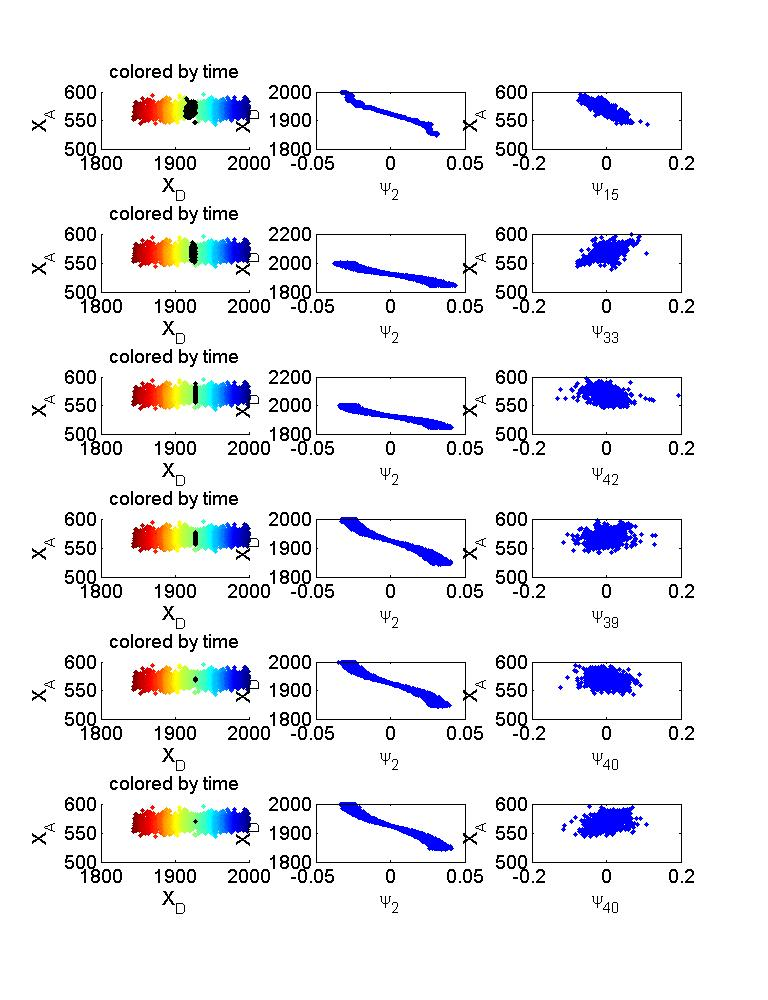
\includegraphics[width=\textwidth]{vary_window_sizes_sde2}
\caption{This is a completely different system (chemical reaction network example)}
\label{fig:1d1drxnnetwork}
\end{figure}

\begin{figure}
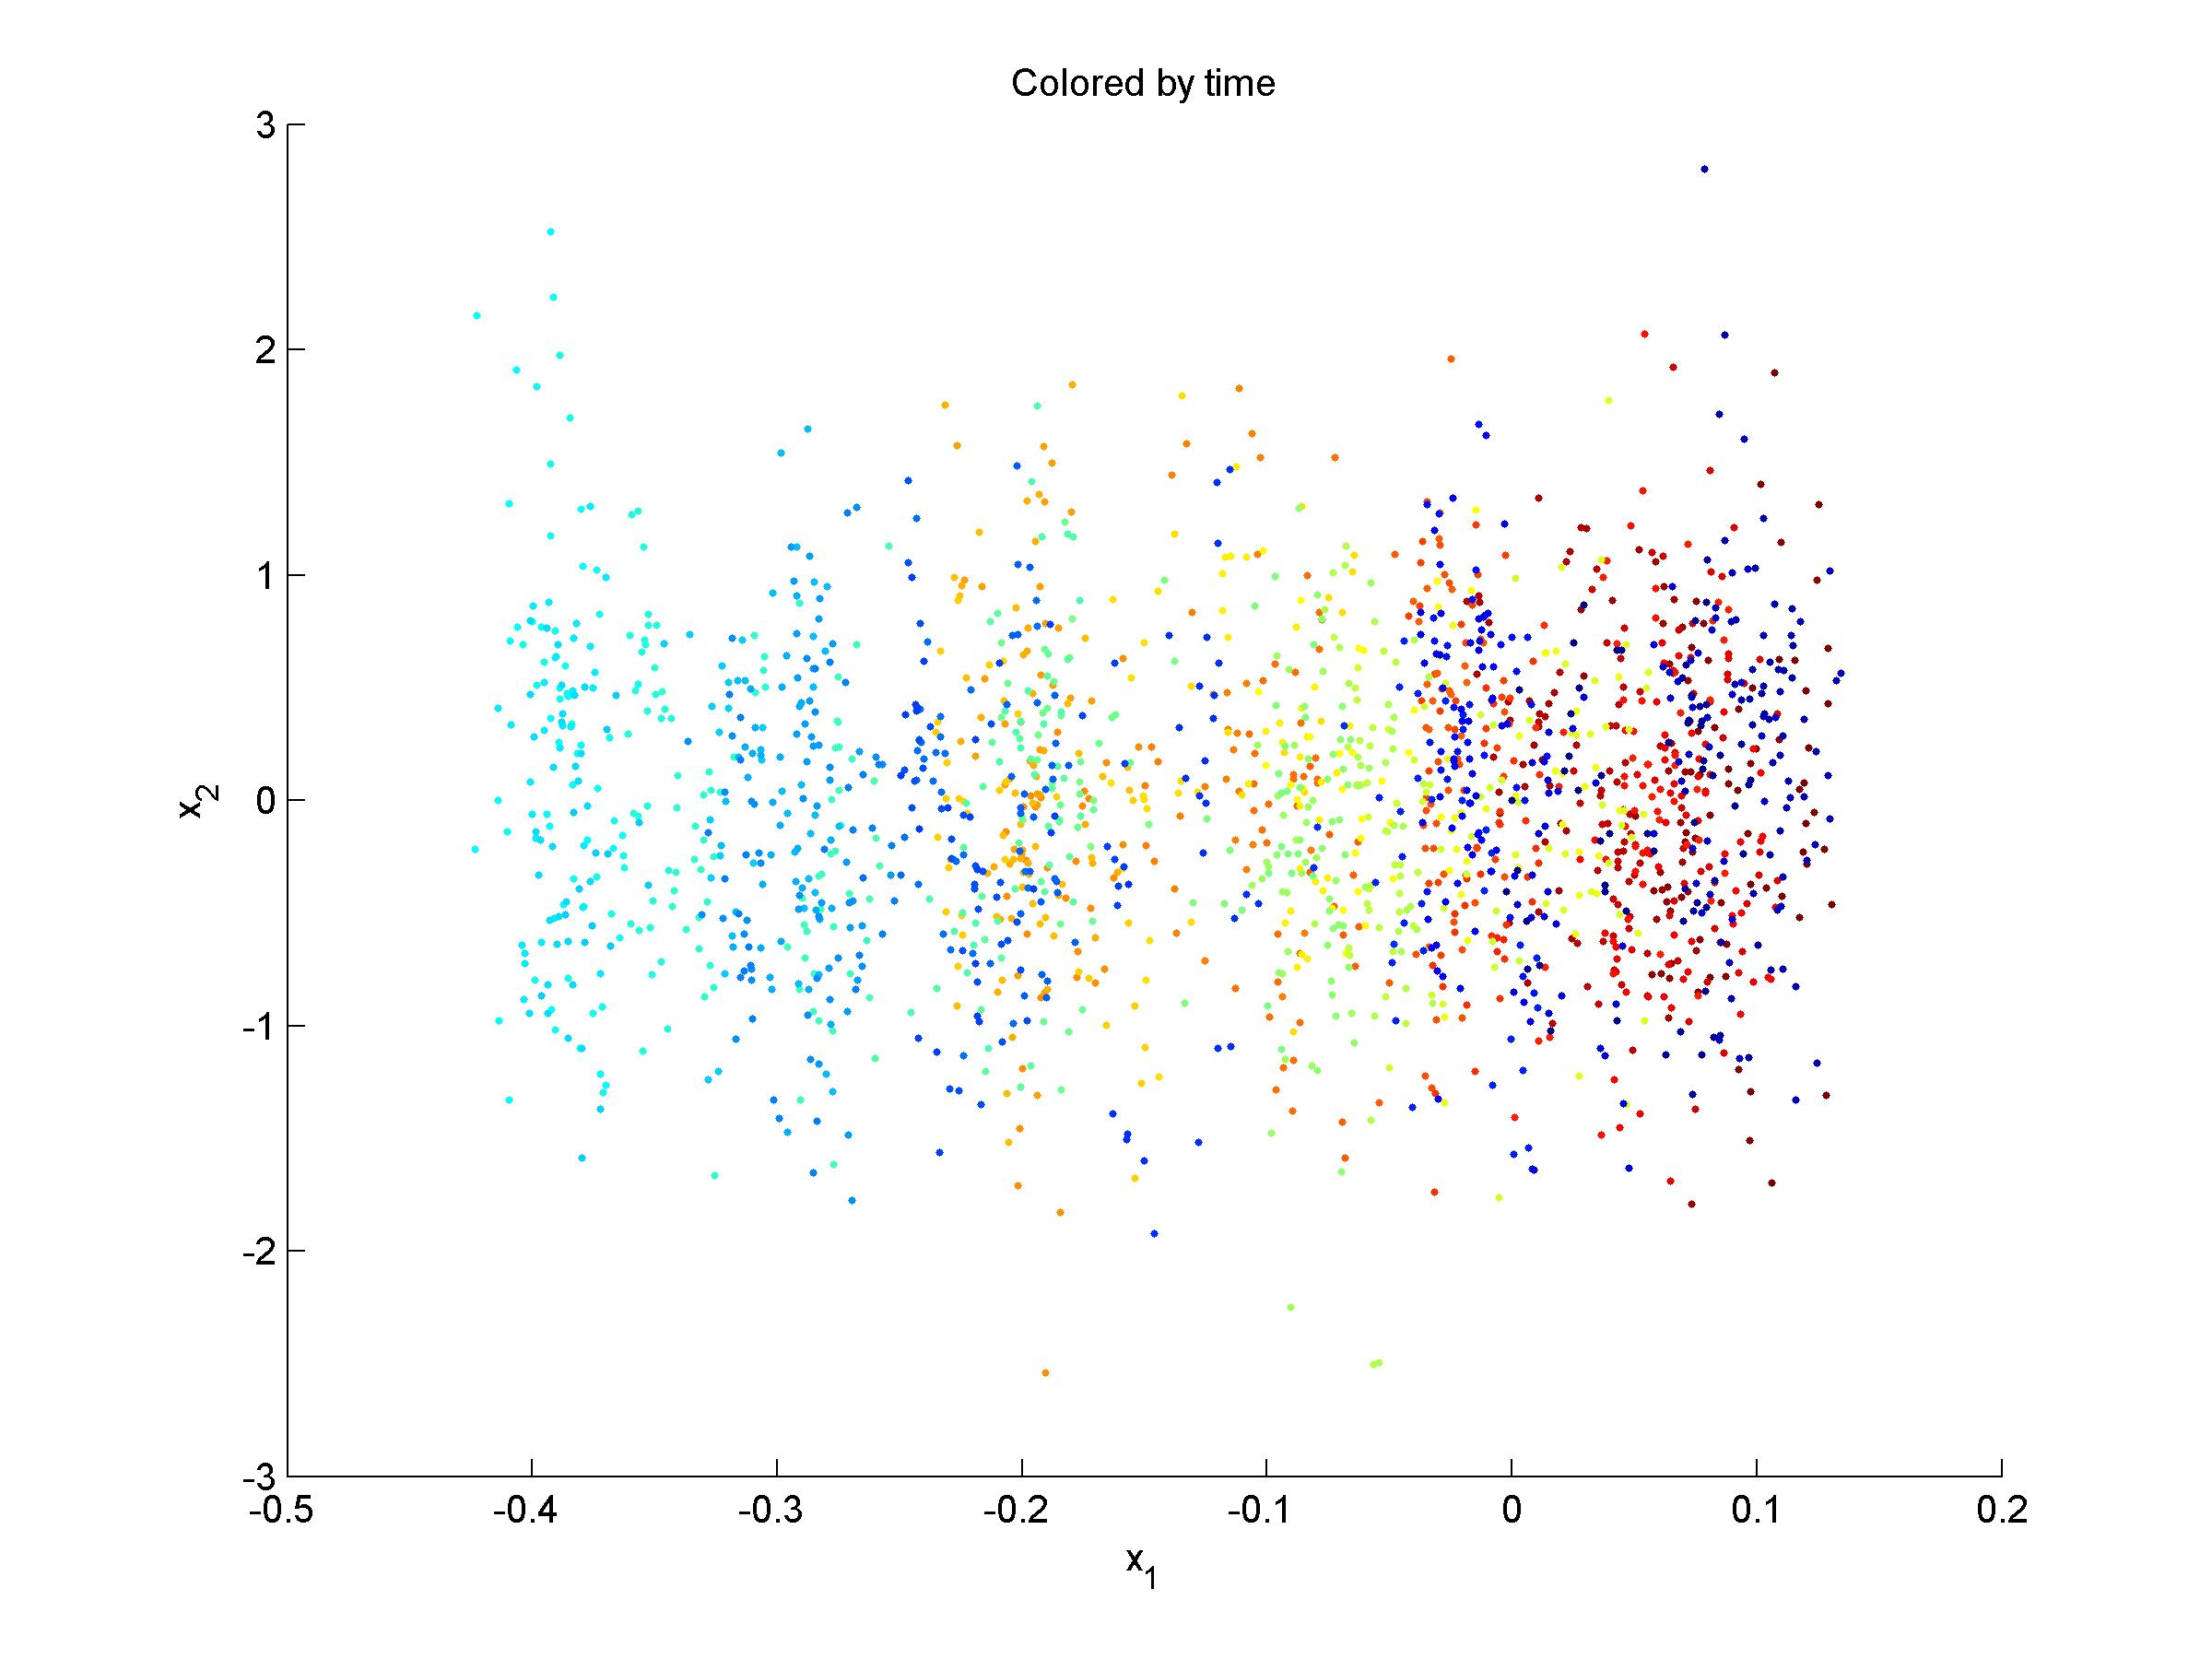
\includegraphics[width=0.5\textwidth]{raw_data} \\
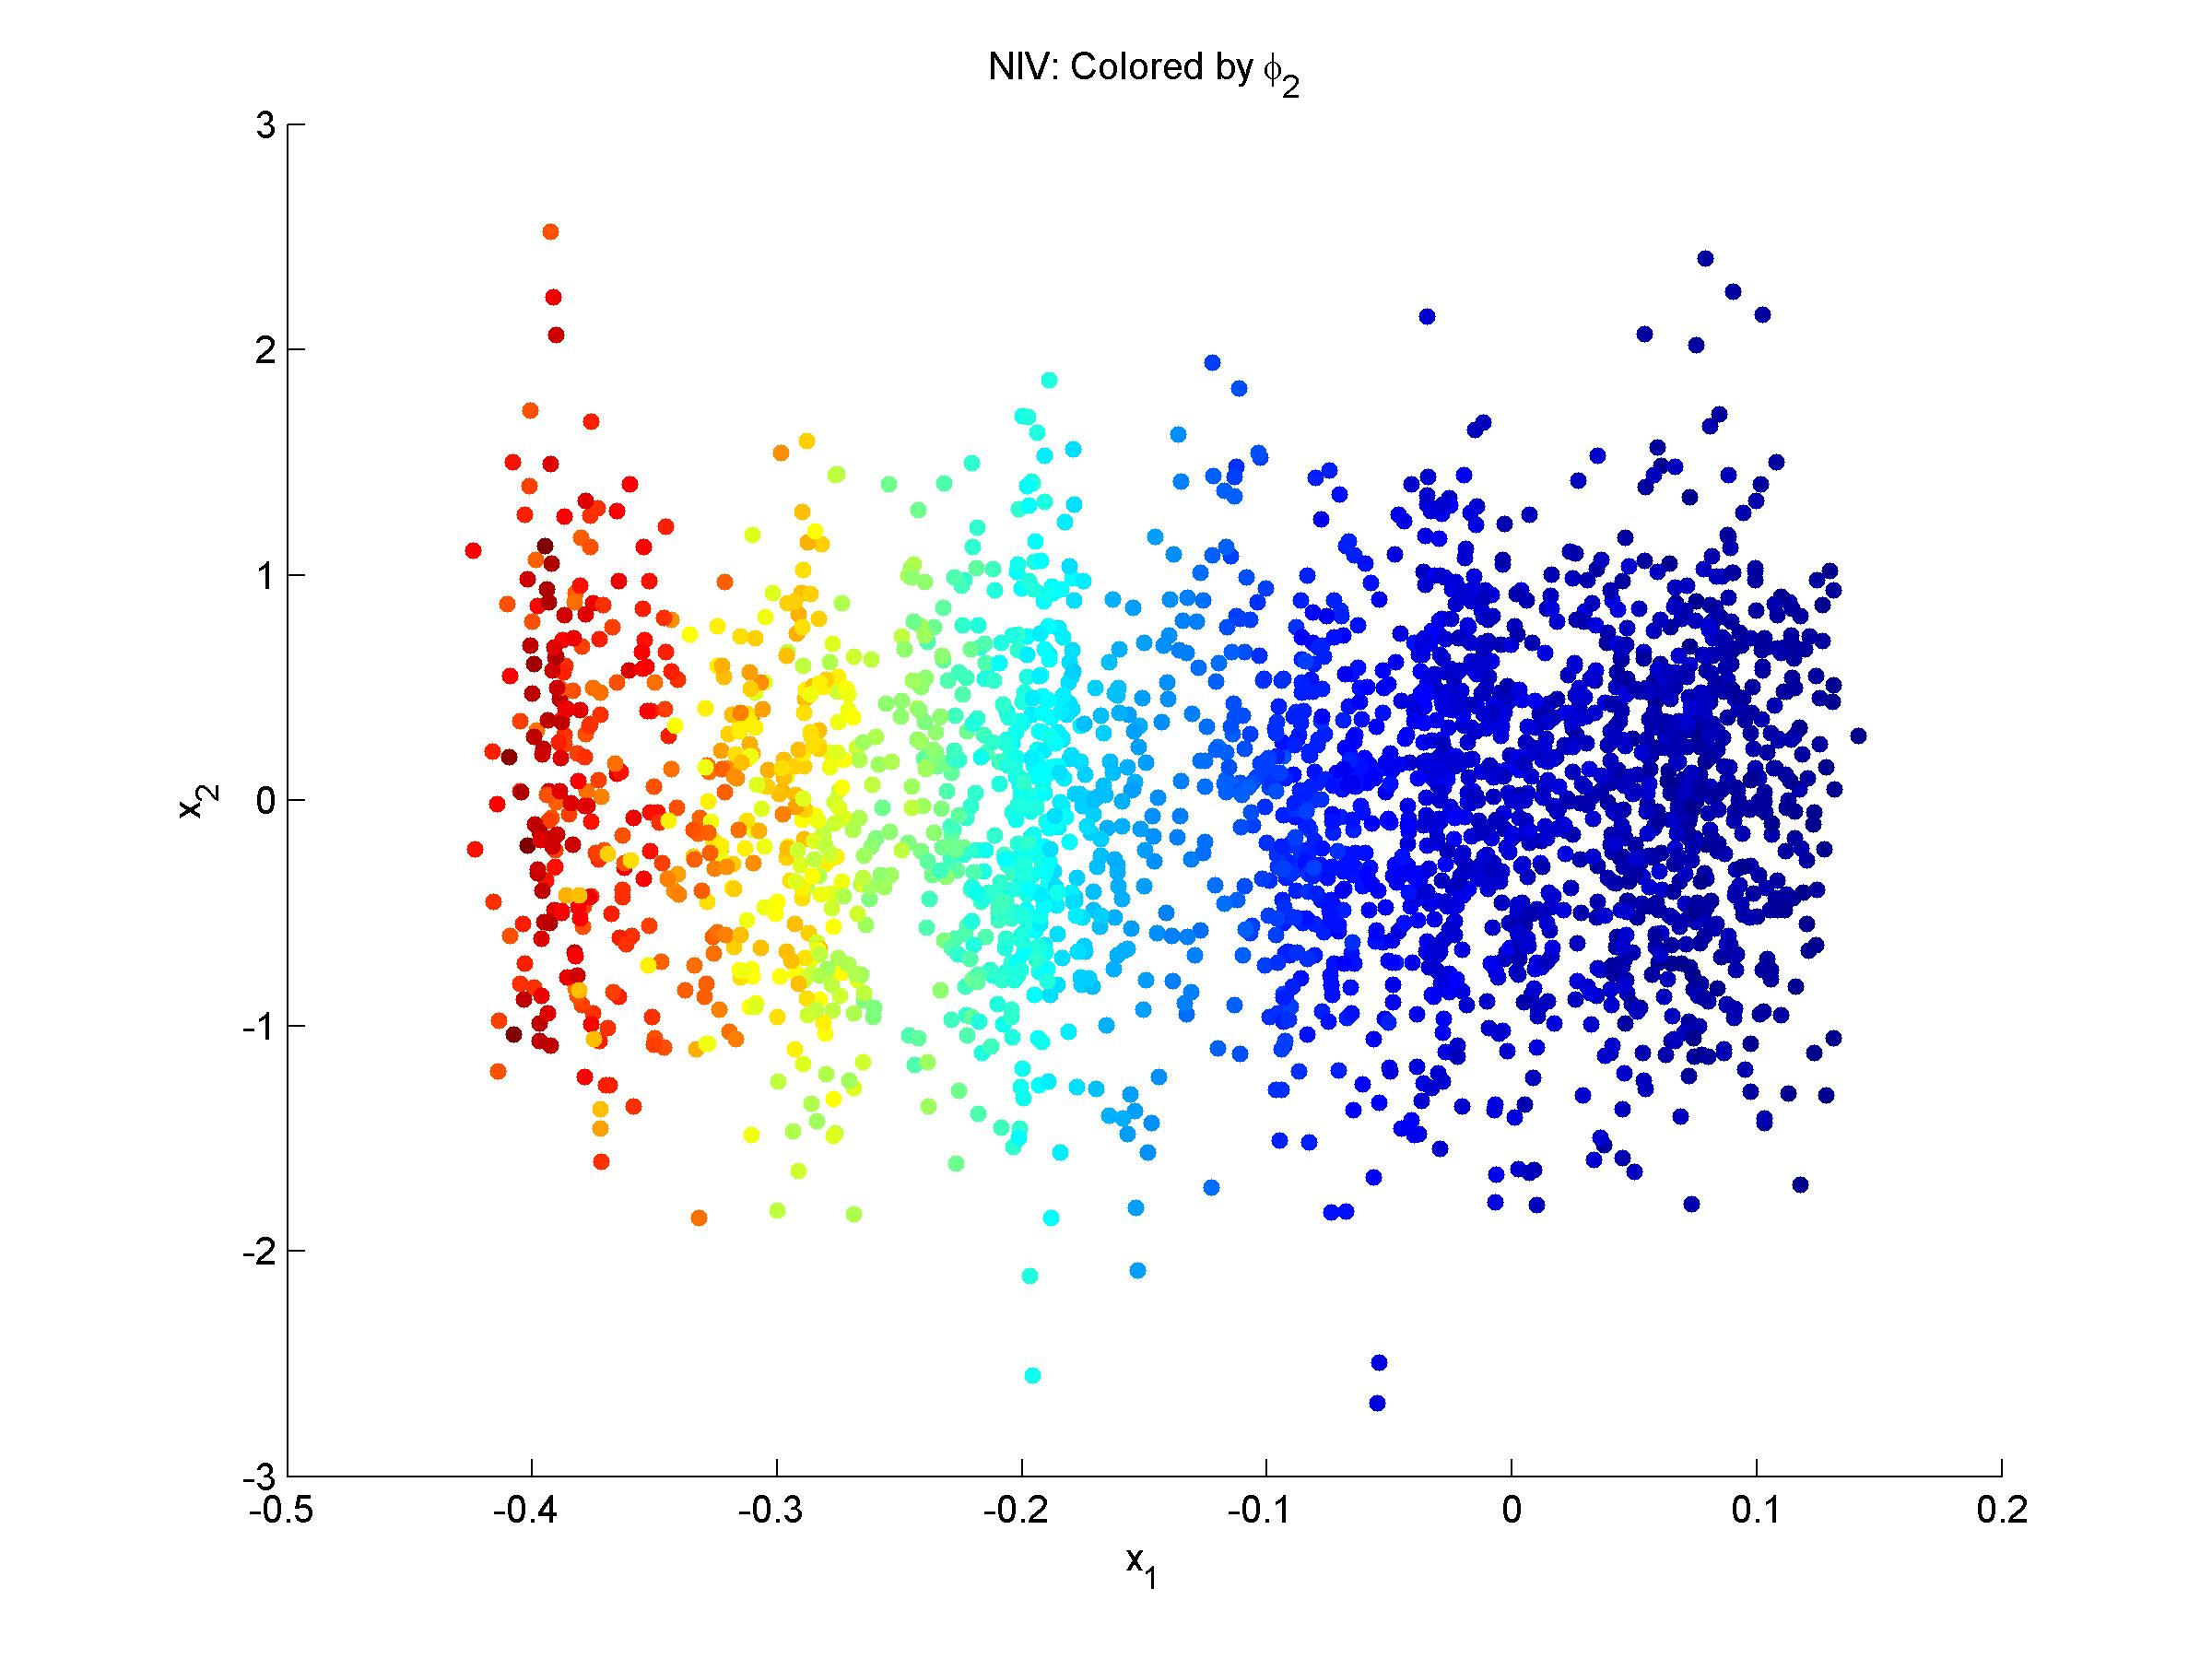
\includegraphics[width=0.5\textwidth]{NIV_data}
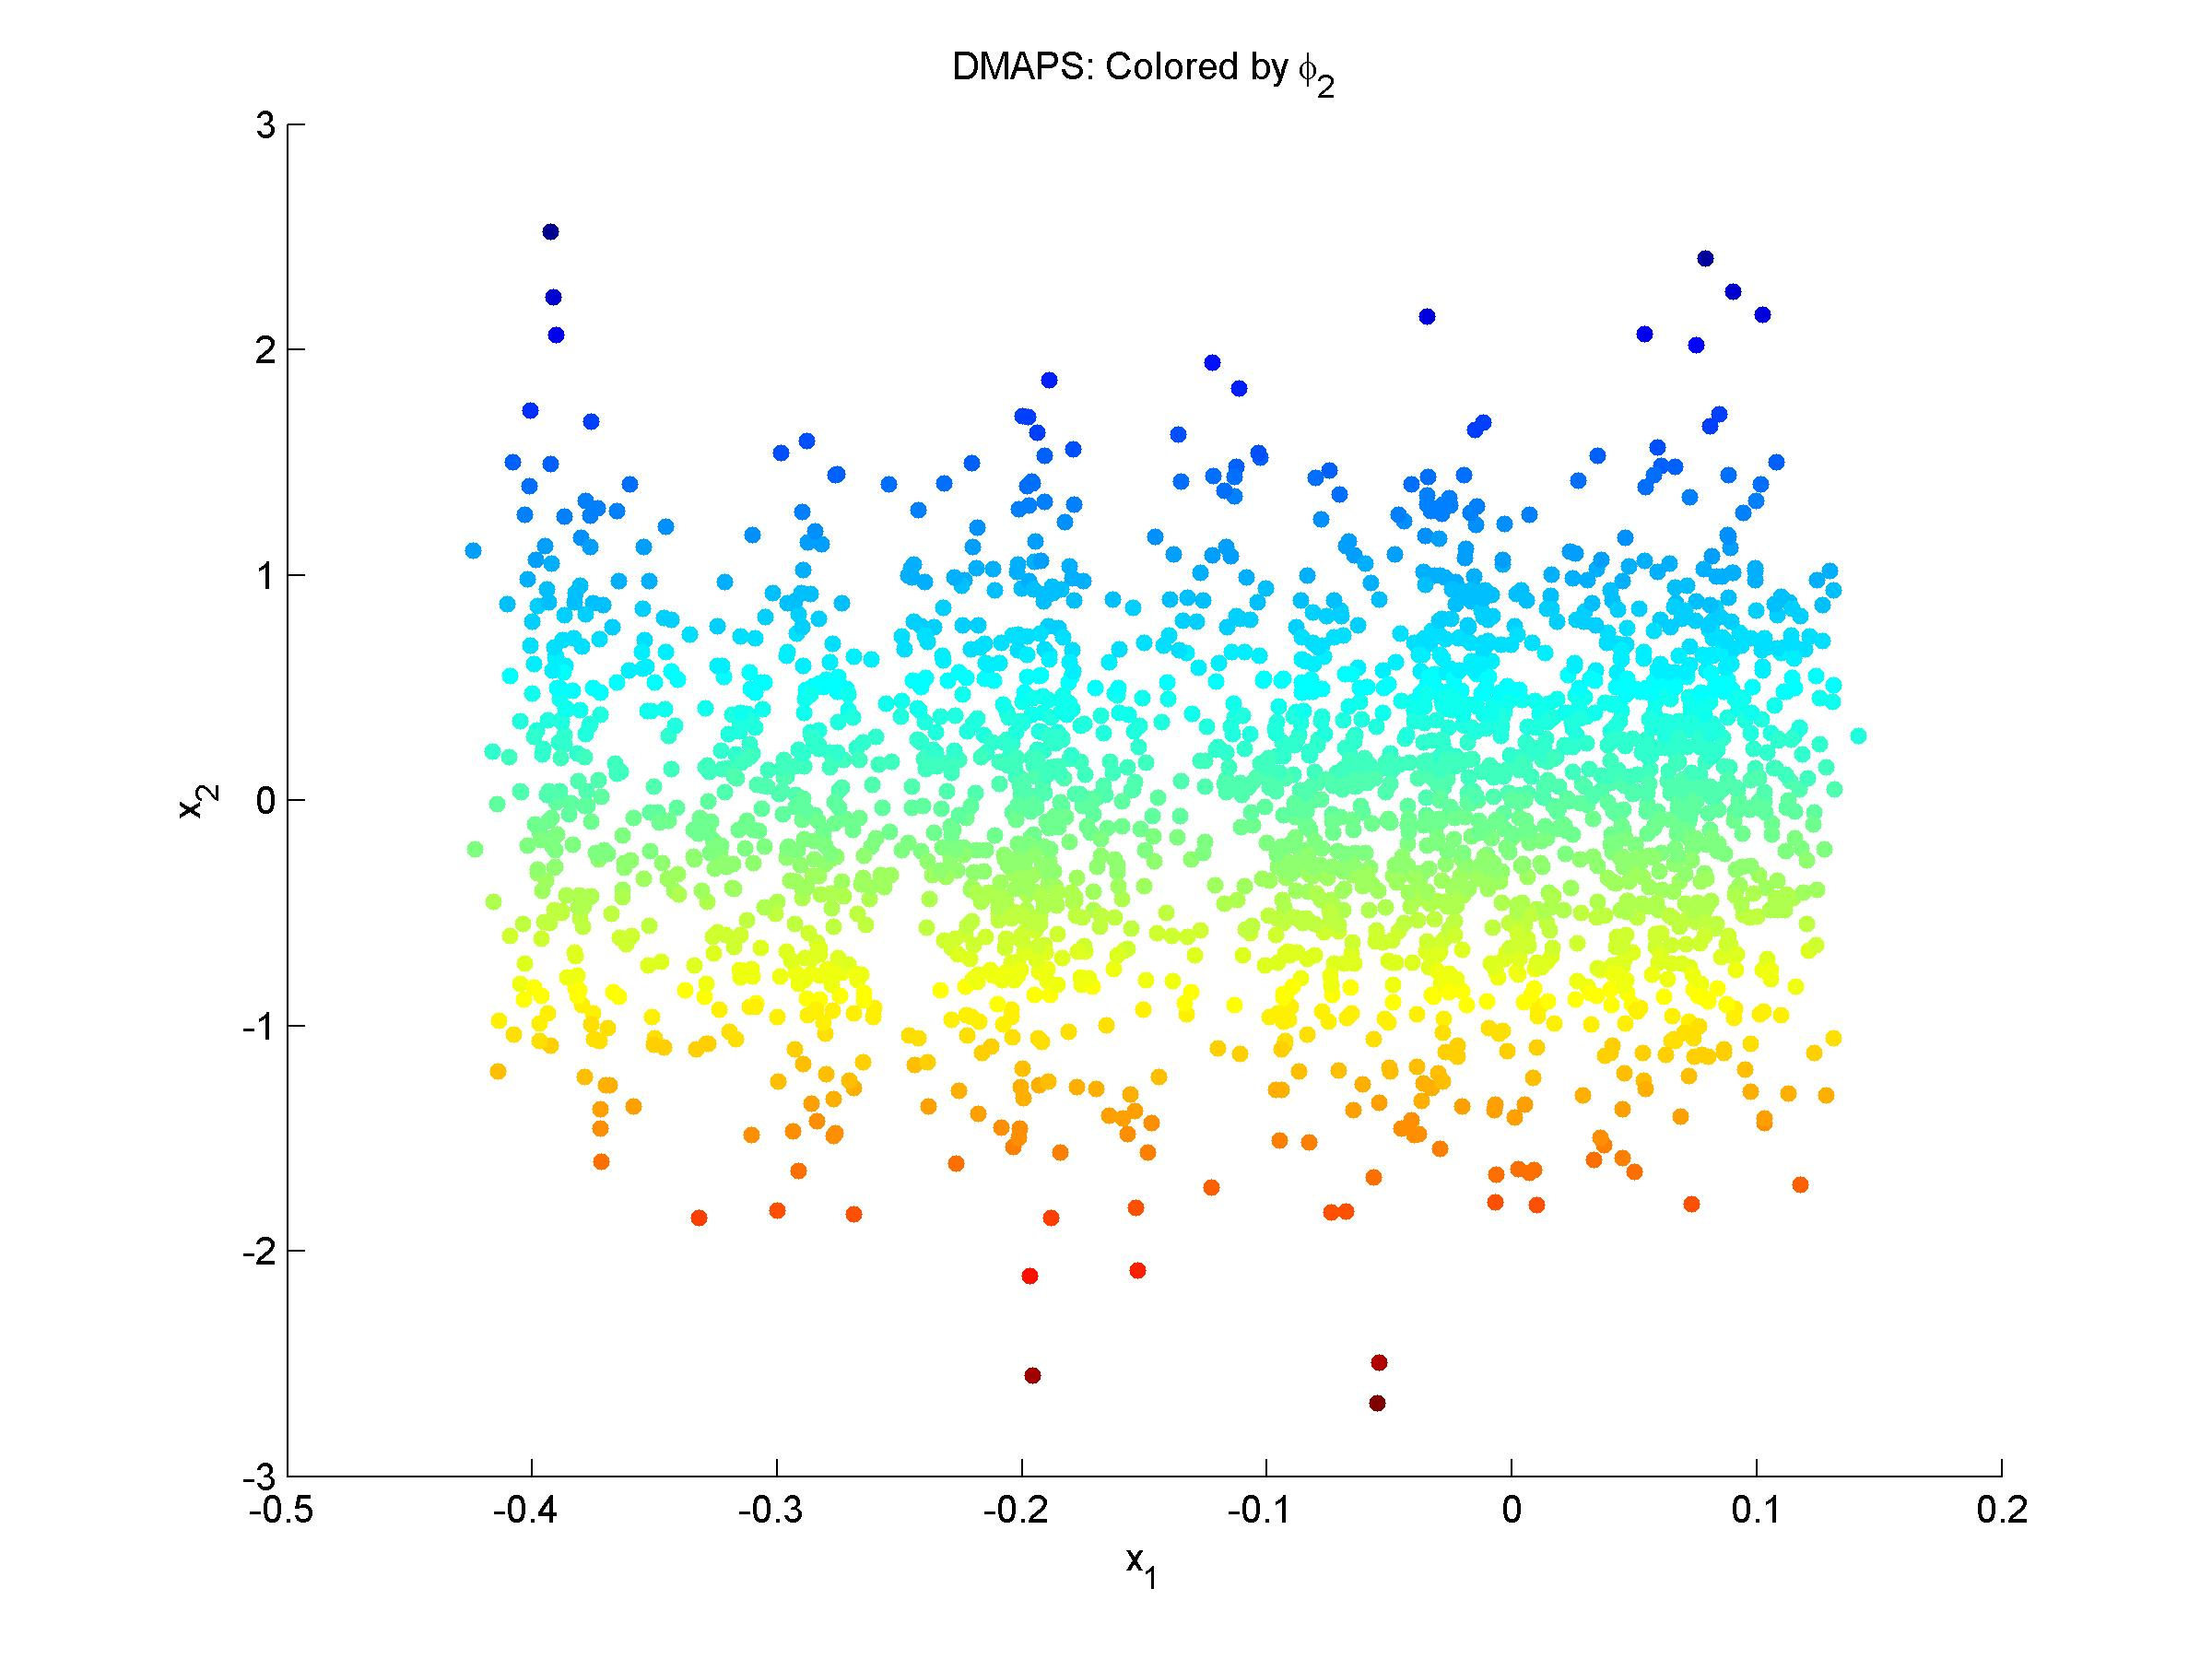
\includegraphics[width=0.5\textwidth]{DMAPS_data}
%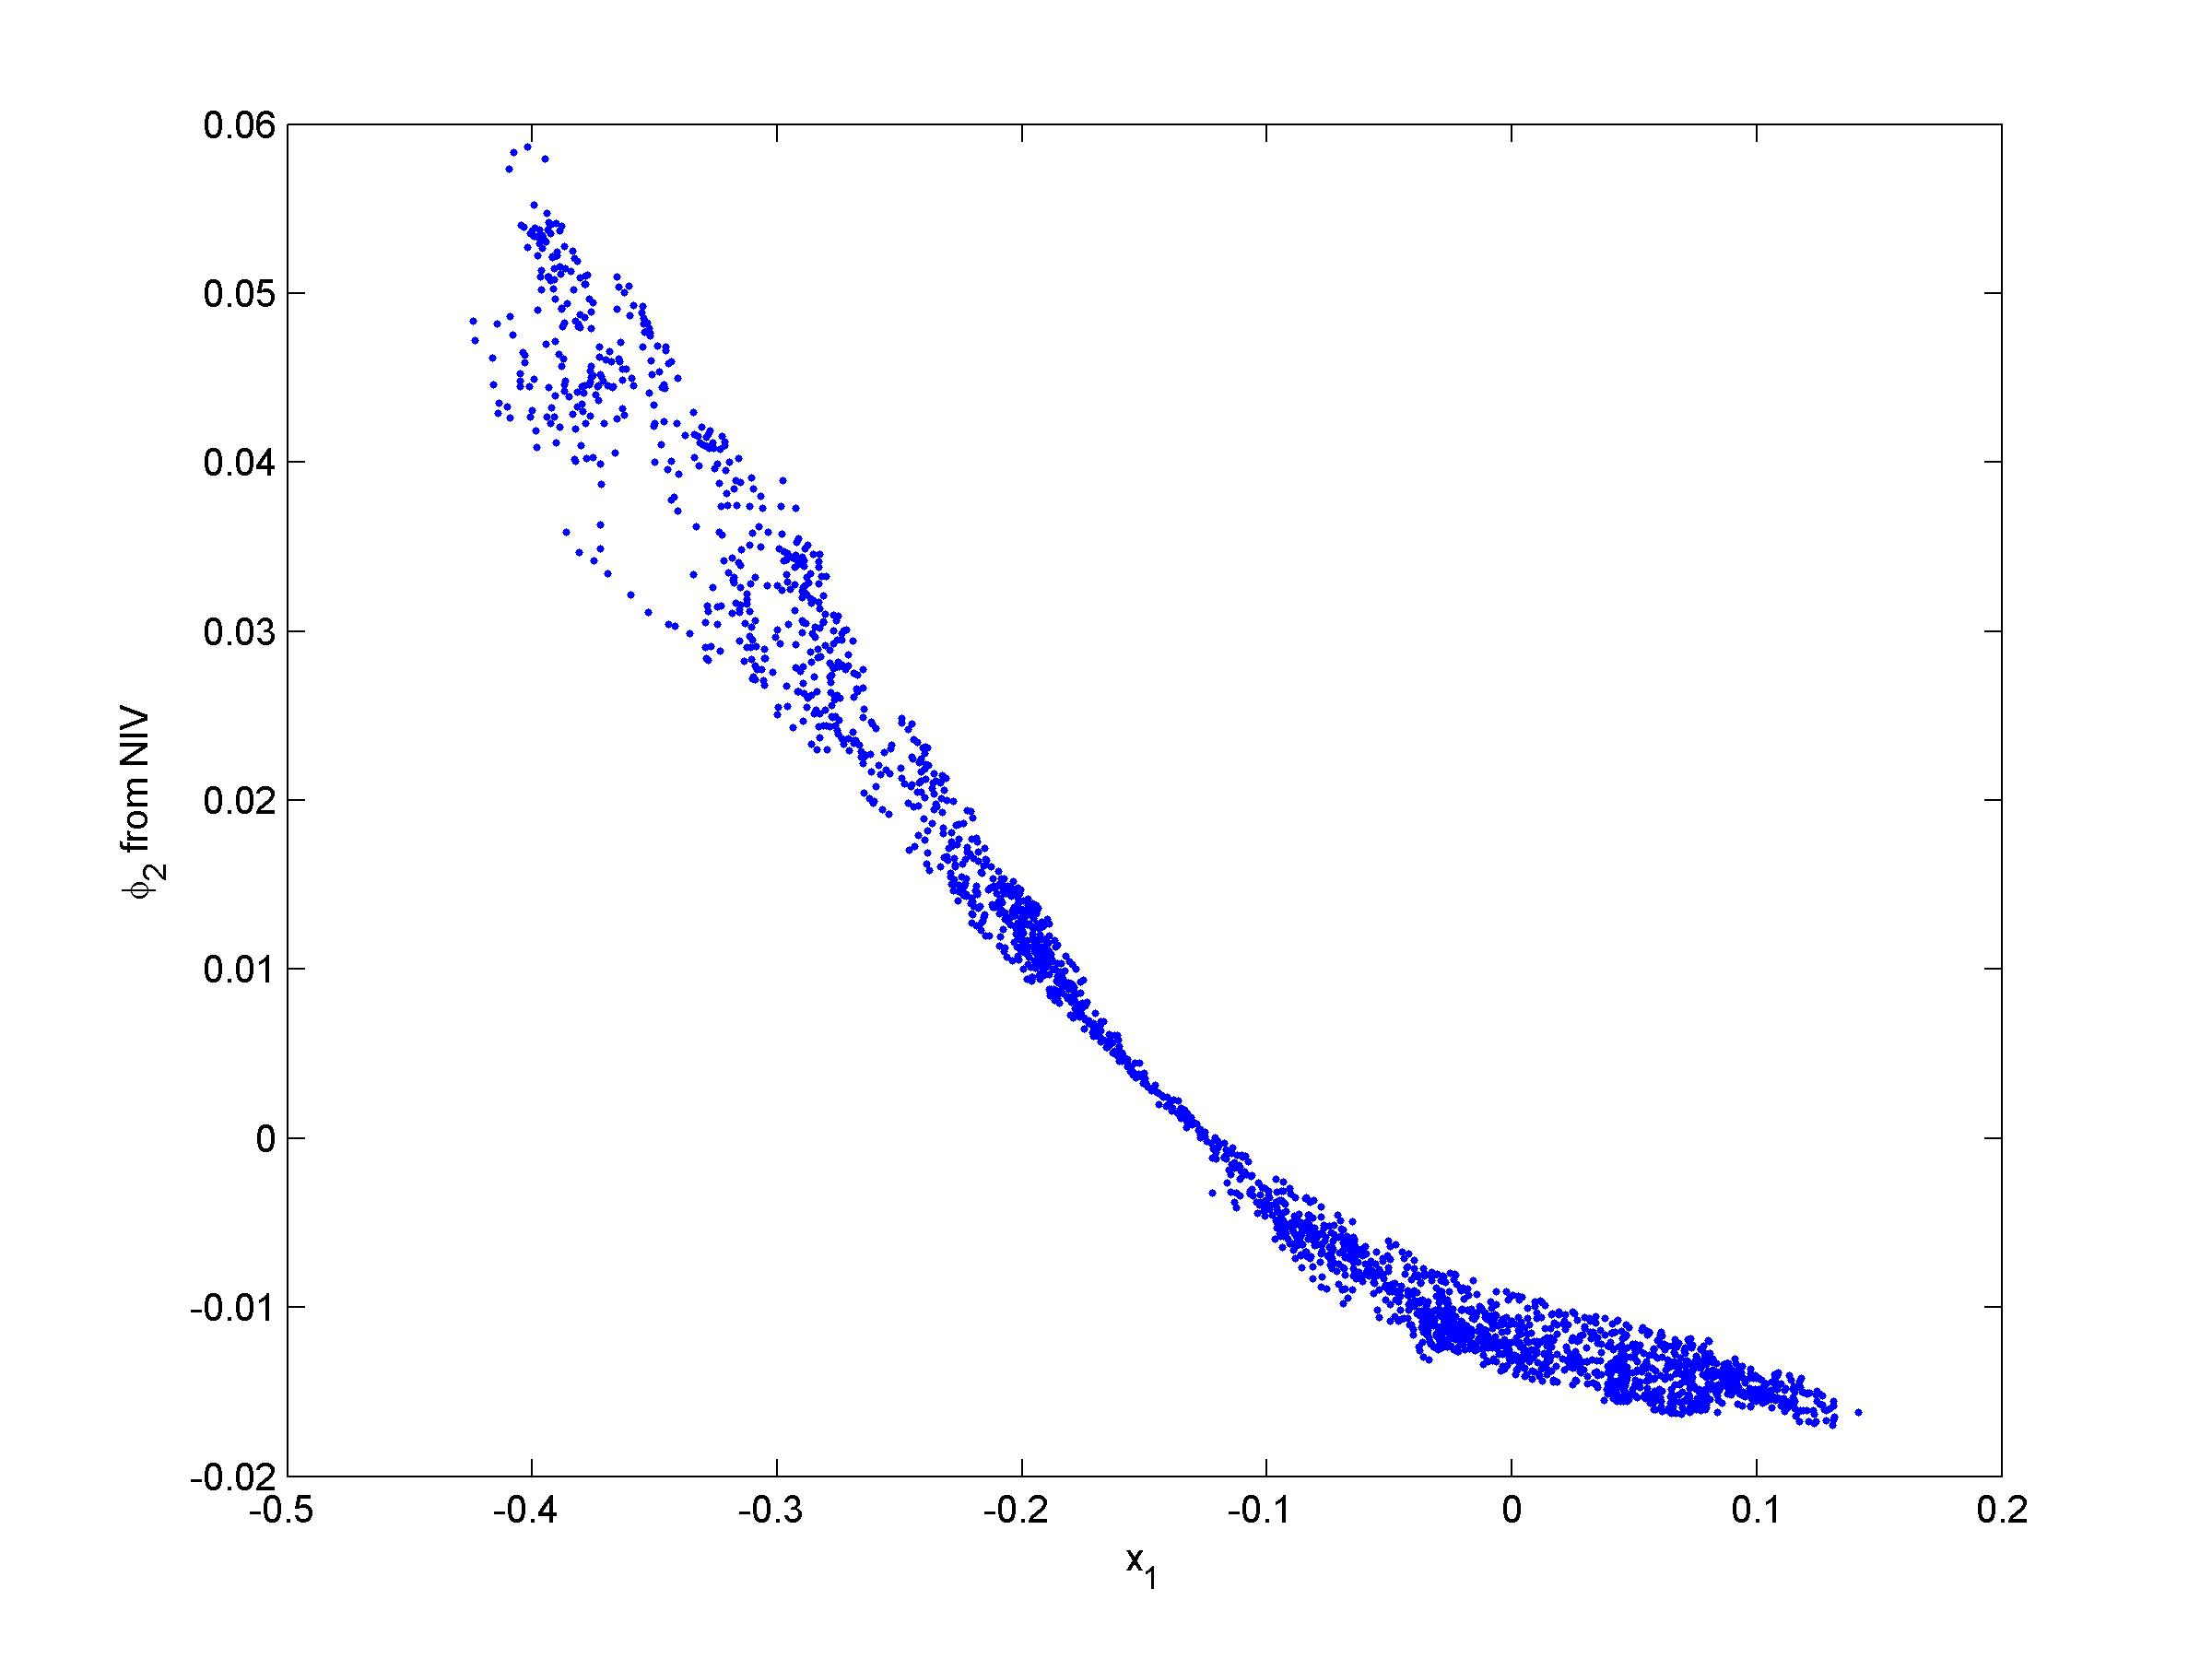
\includegraphics[width=0.5\textwidth]{NIV_corr}
%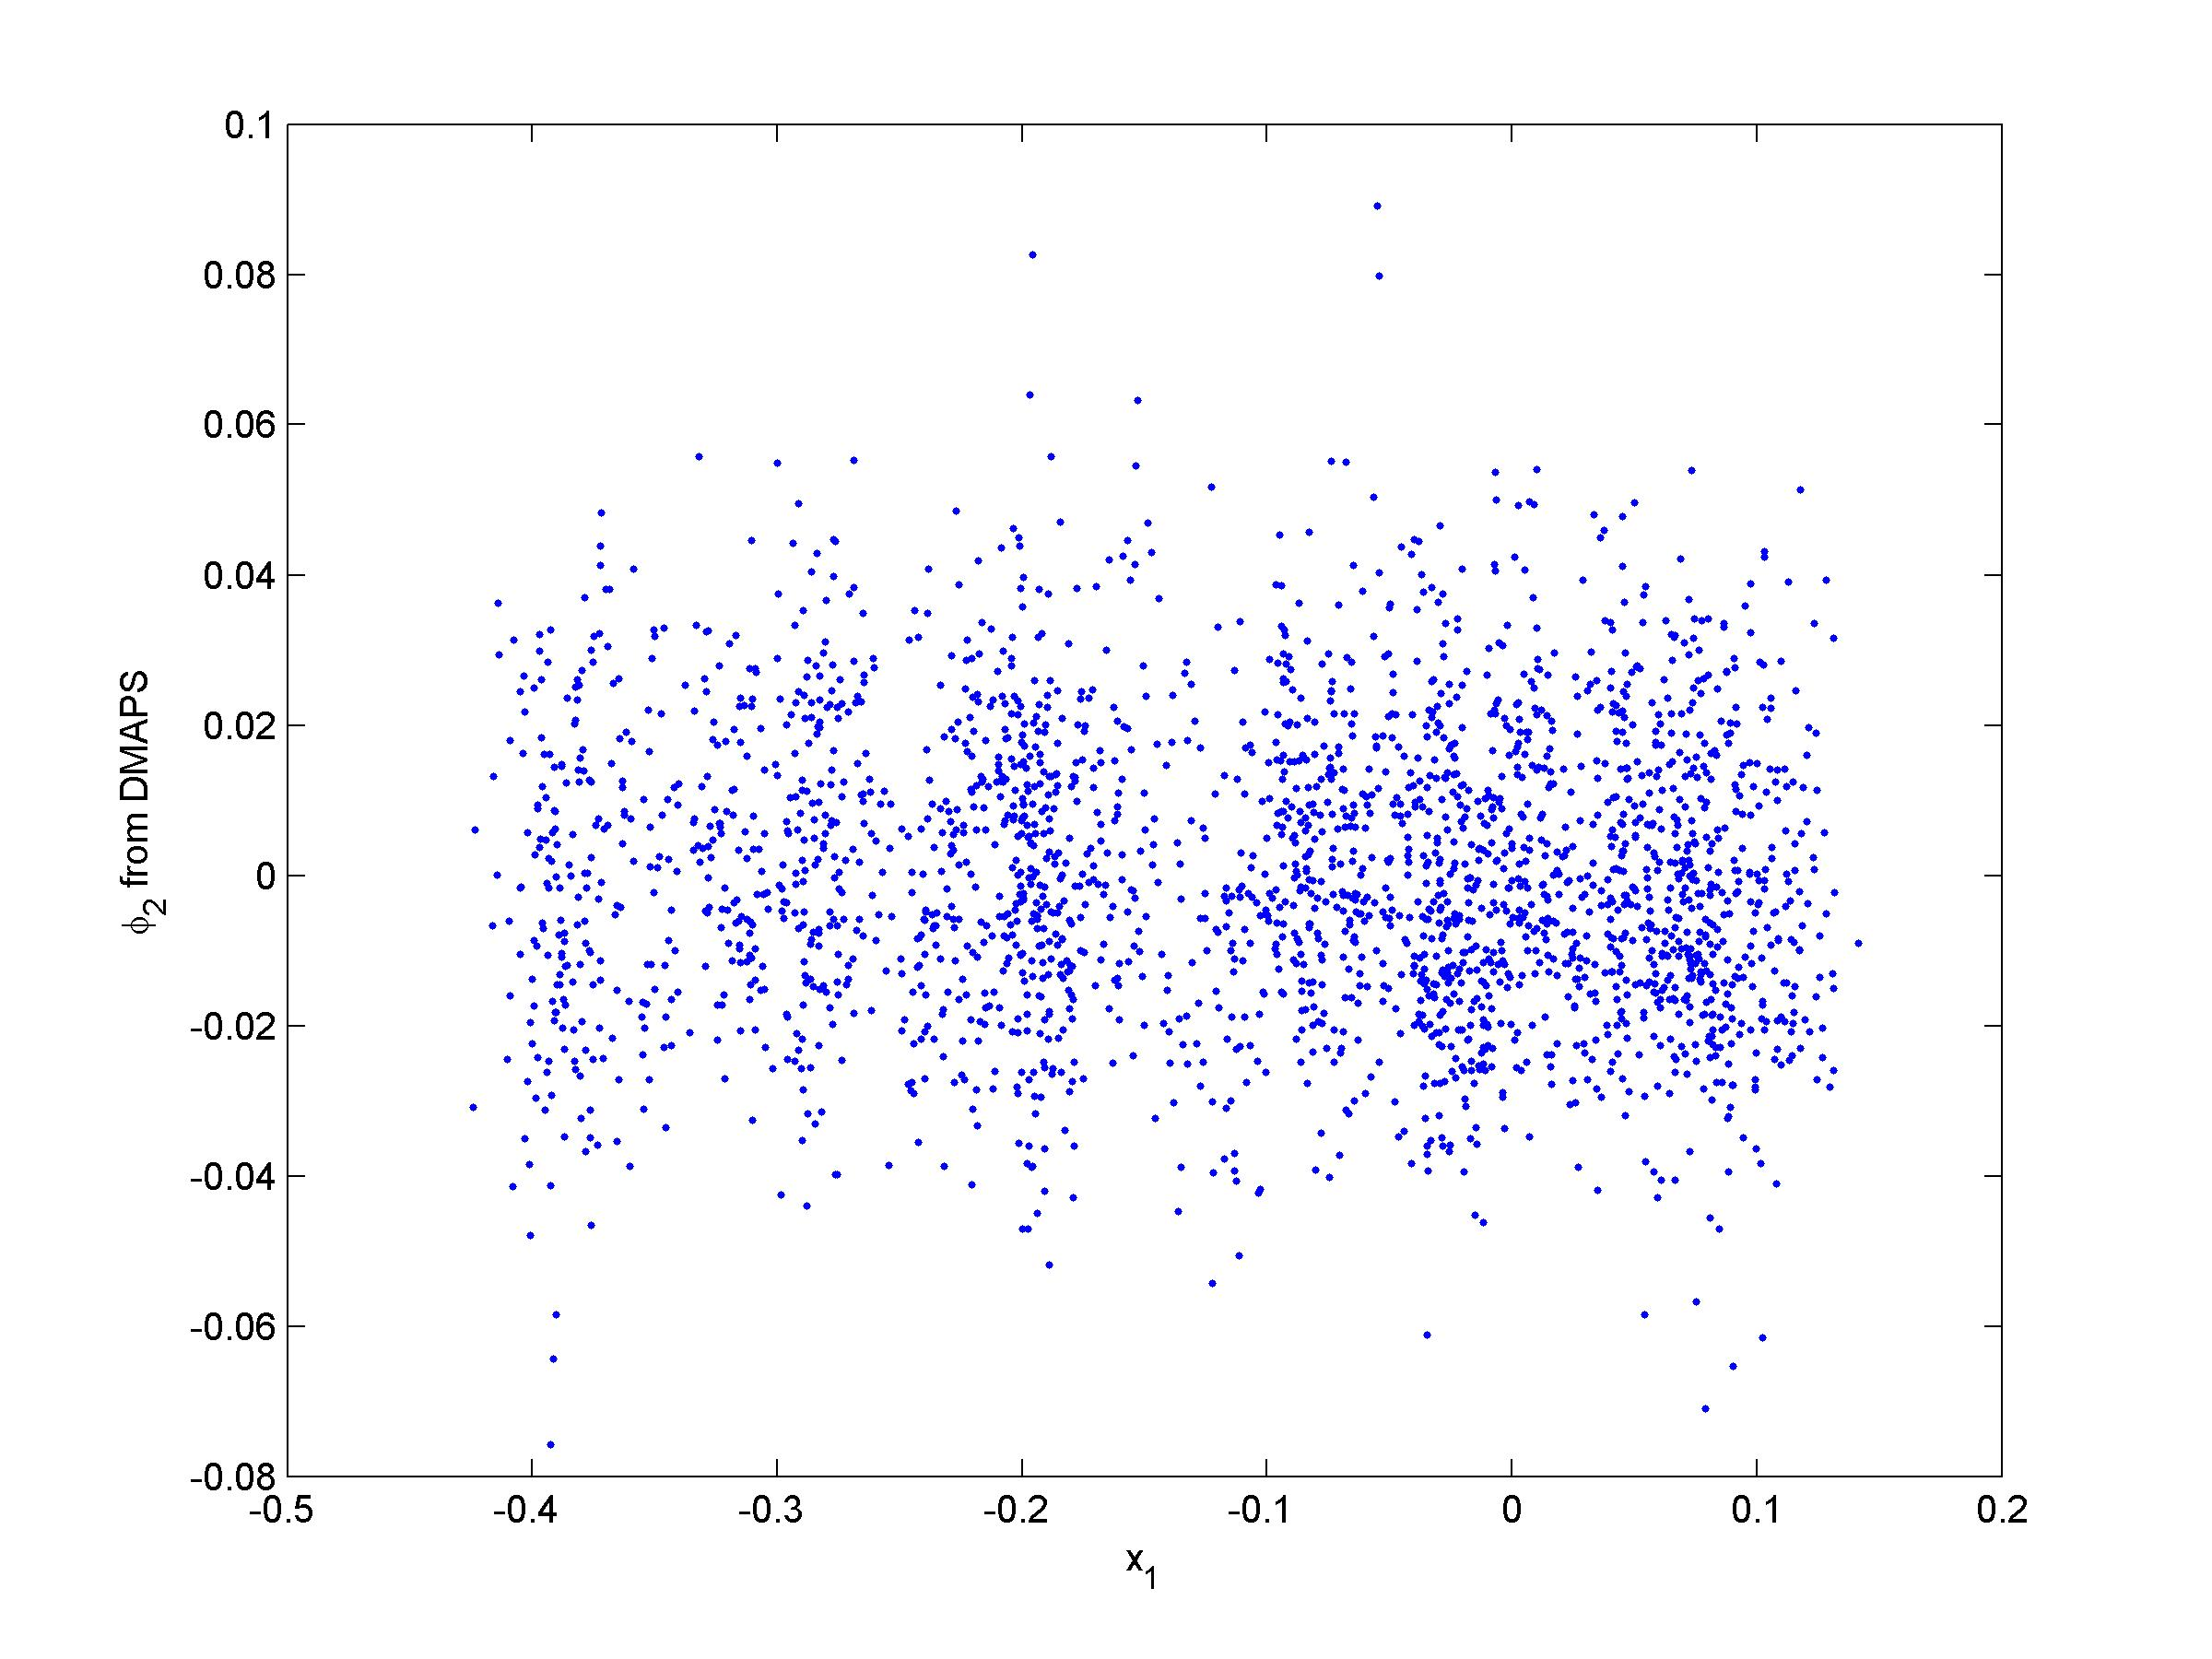
\includegraphics[width=0.5\textwidth]{DMAPS_corr}
%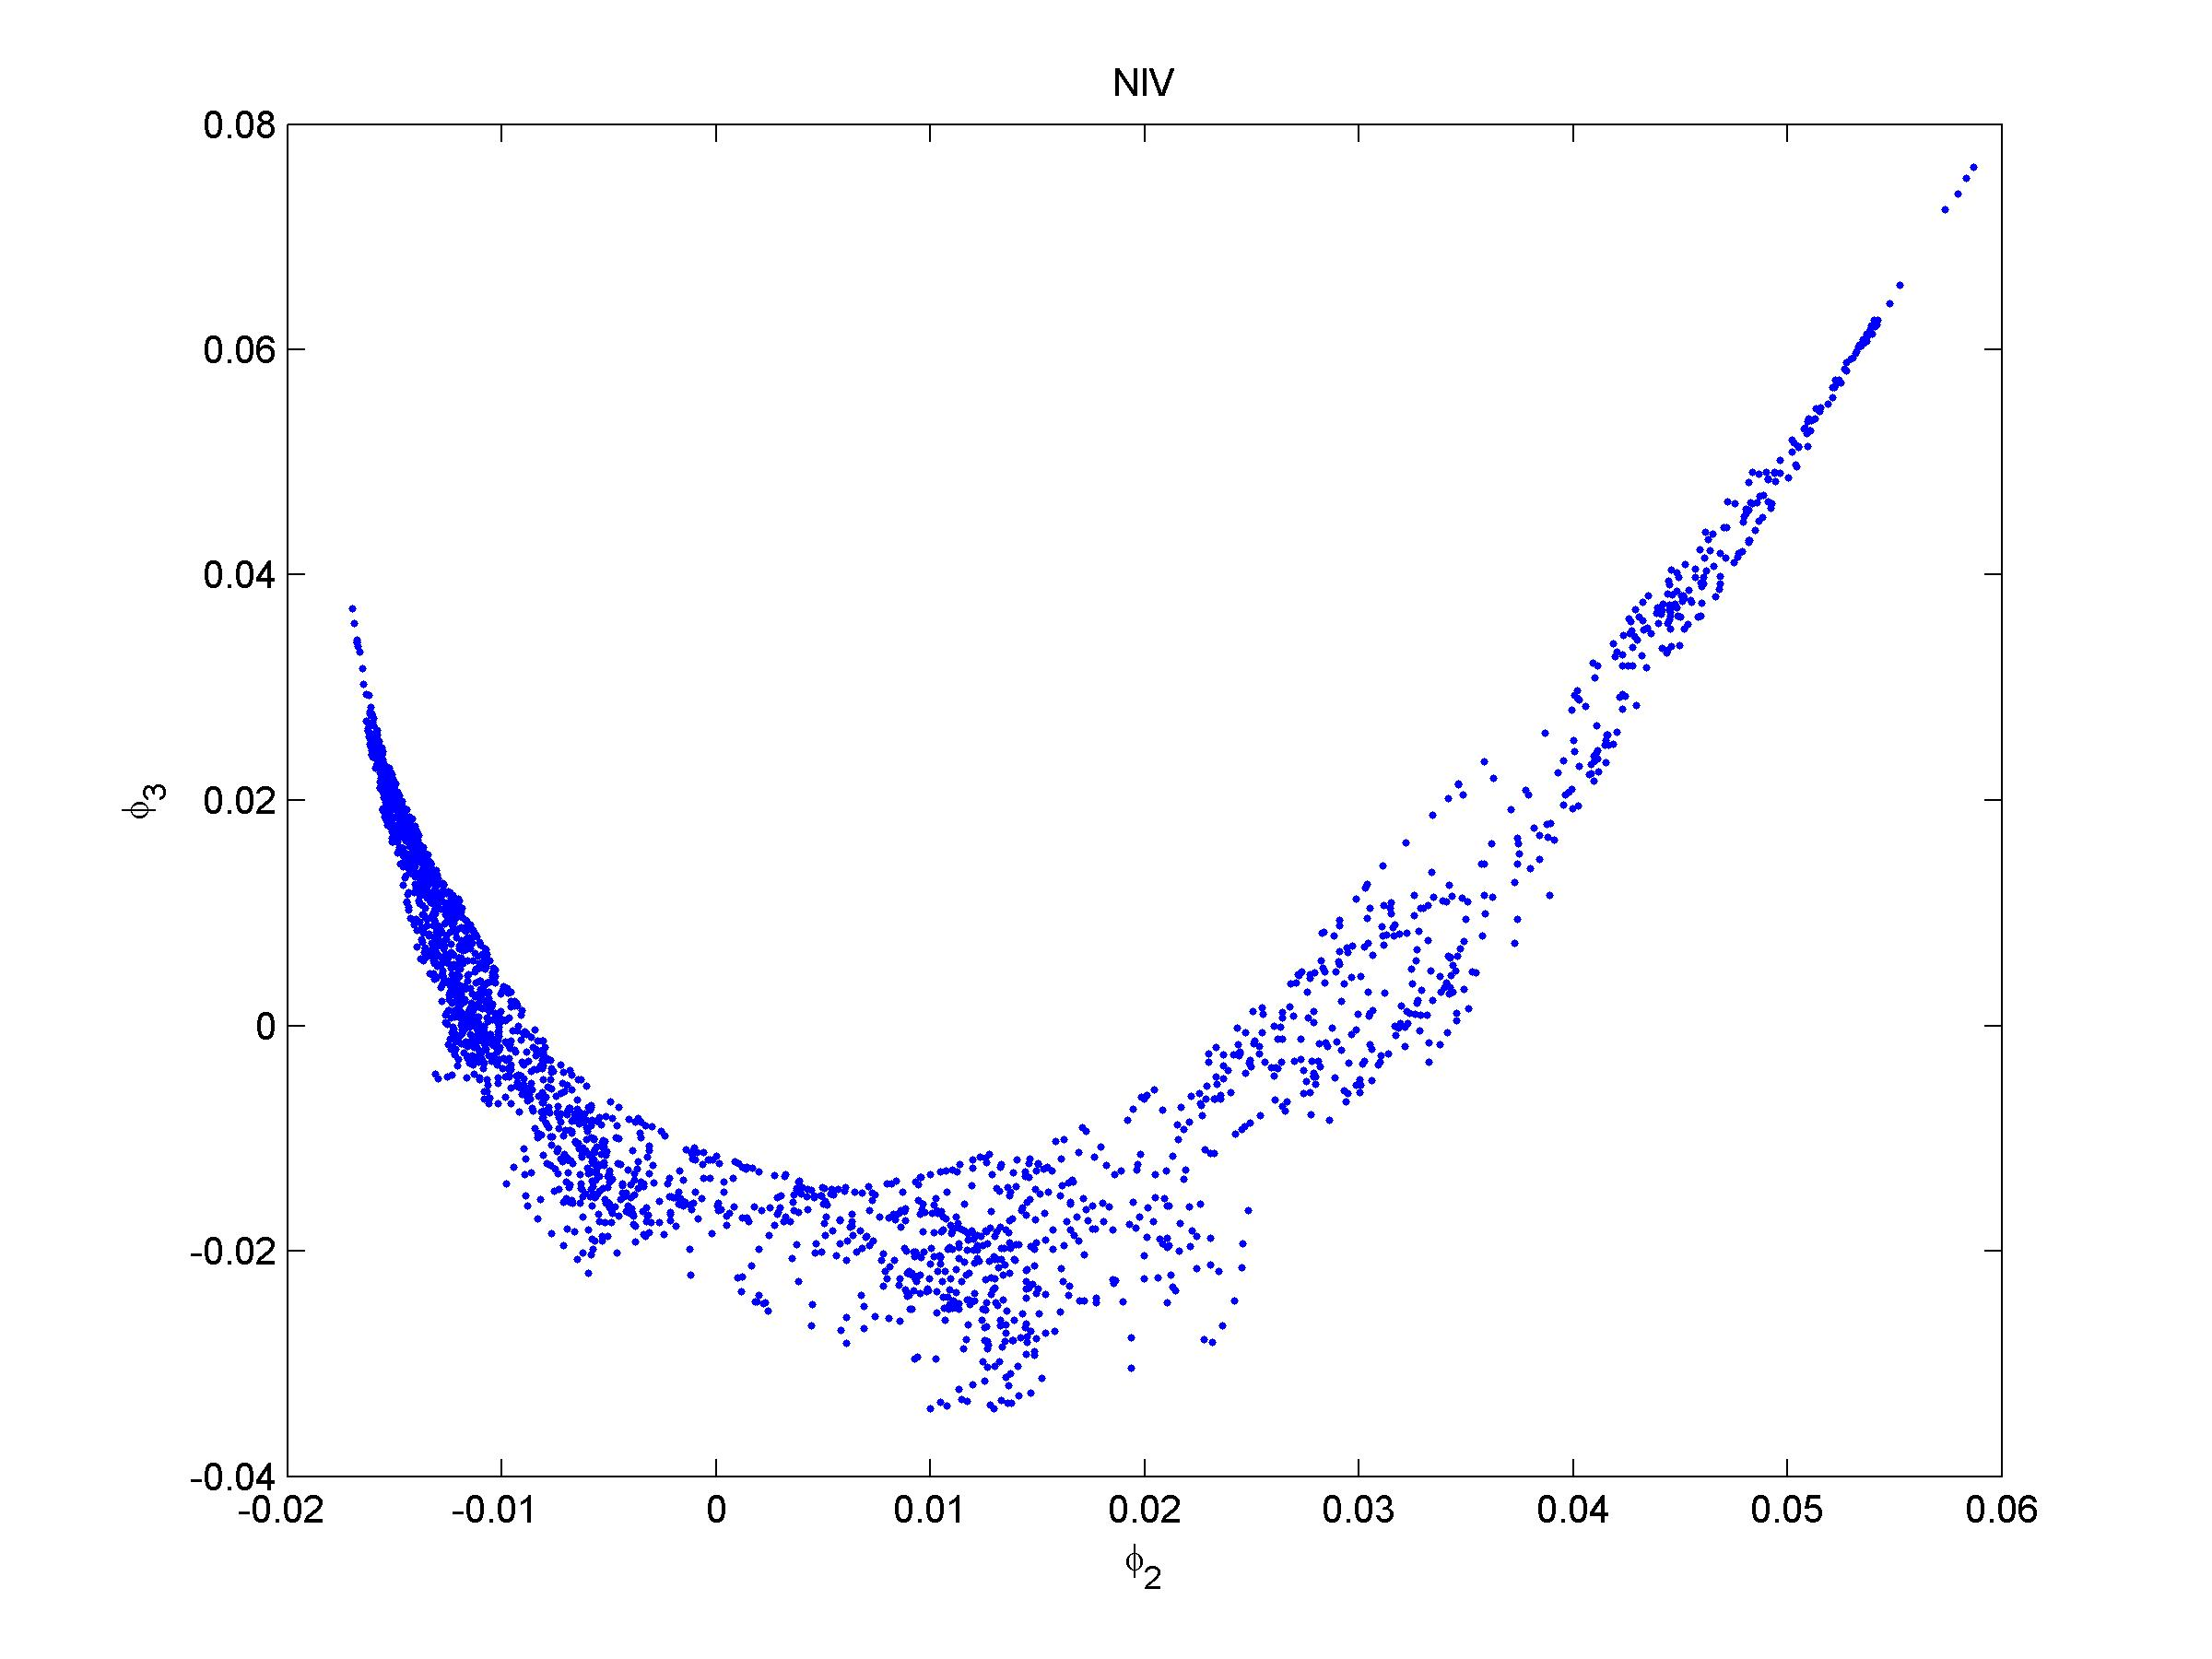
\includegraphics[width=0.5\textwidth]{NIV_embed}
%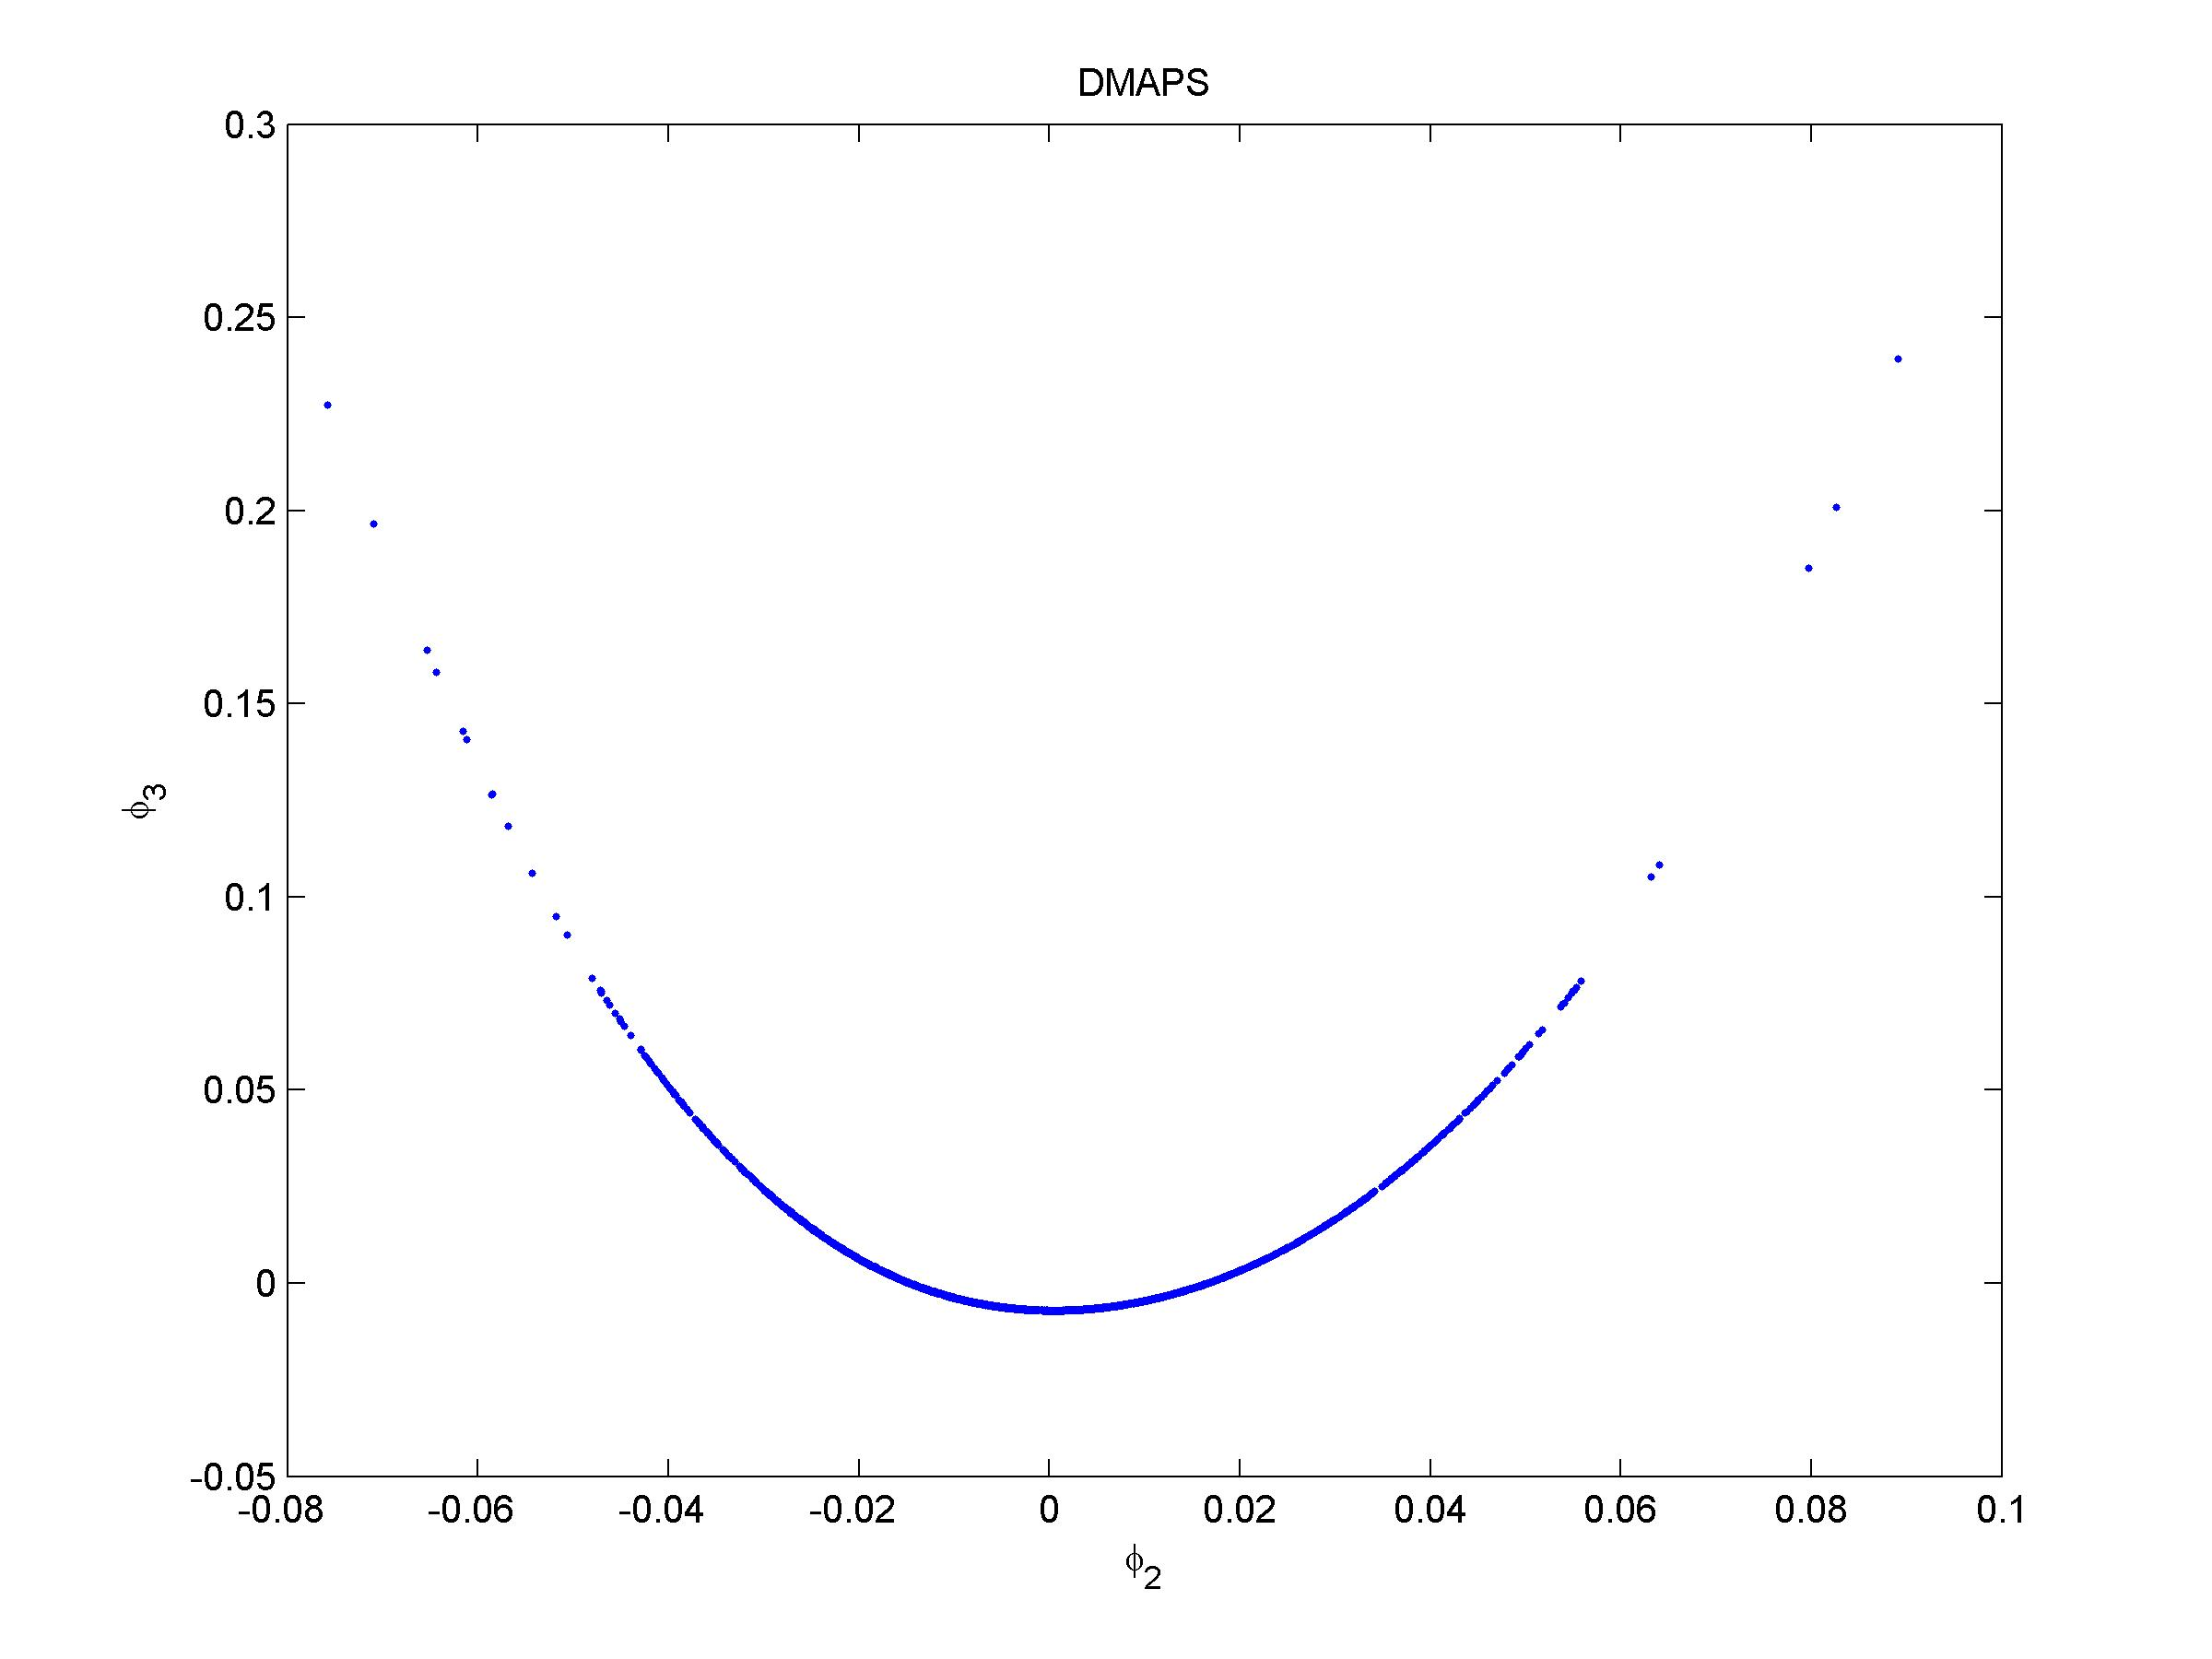
\includegraphics[width=0.5\textwidth]{DMAPS_embed}
\caption{Top: raw data, colored by time. Bottom, left: Raw data, colored by first NIV. The first NIV captures the slow variable. We use $\epsilon = 0.0001$, $dt = 0.00001$, and time window $0.001$. Bottom, right: Raw data, colored by first DMAPS. The first DMAPS captures the fast variable. test\_scale\_separation.m} 
\label{fig:1d1dexample}
\end{figure}

\begin{figure}
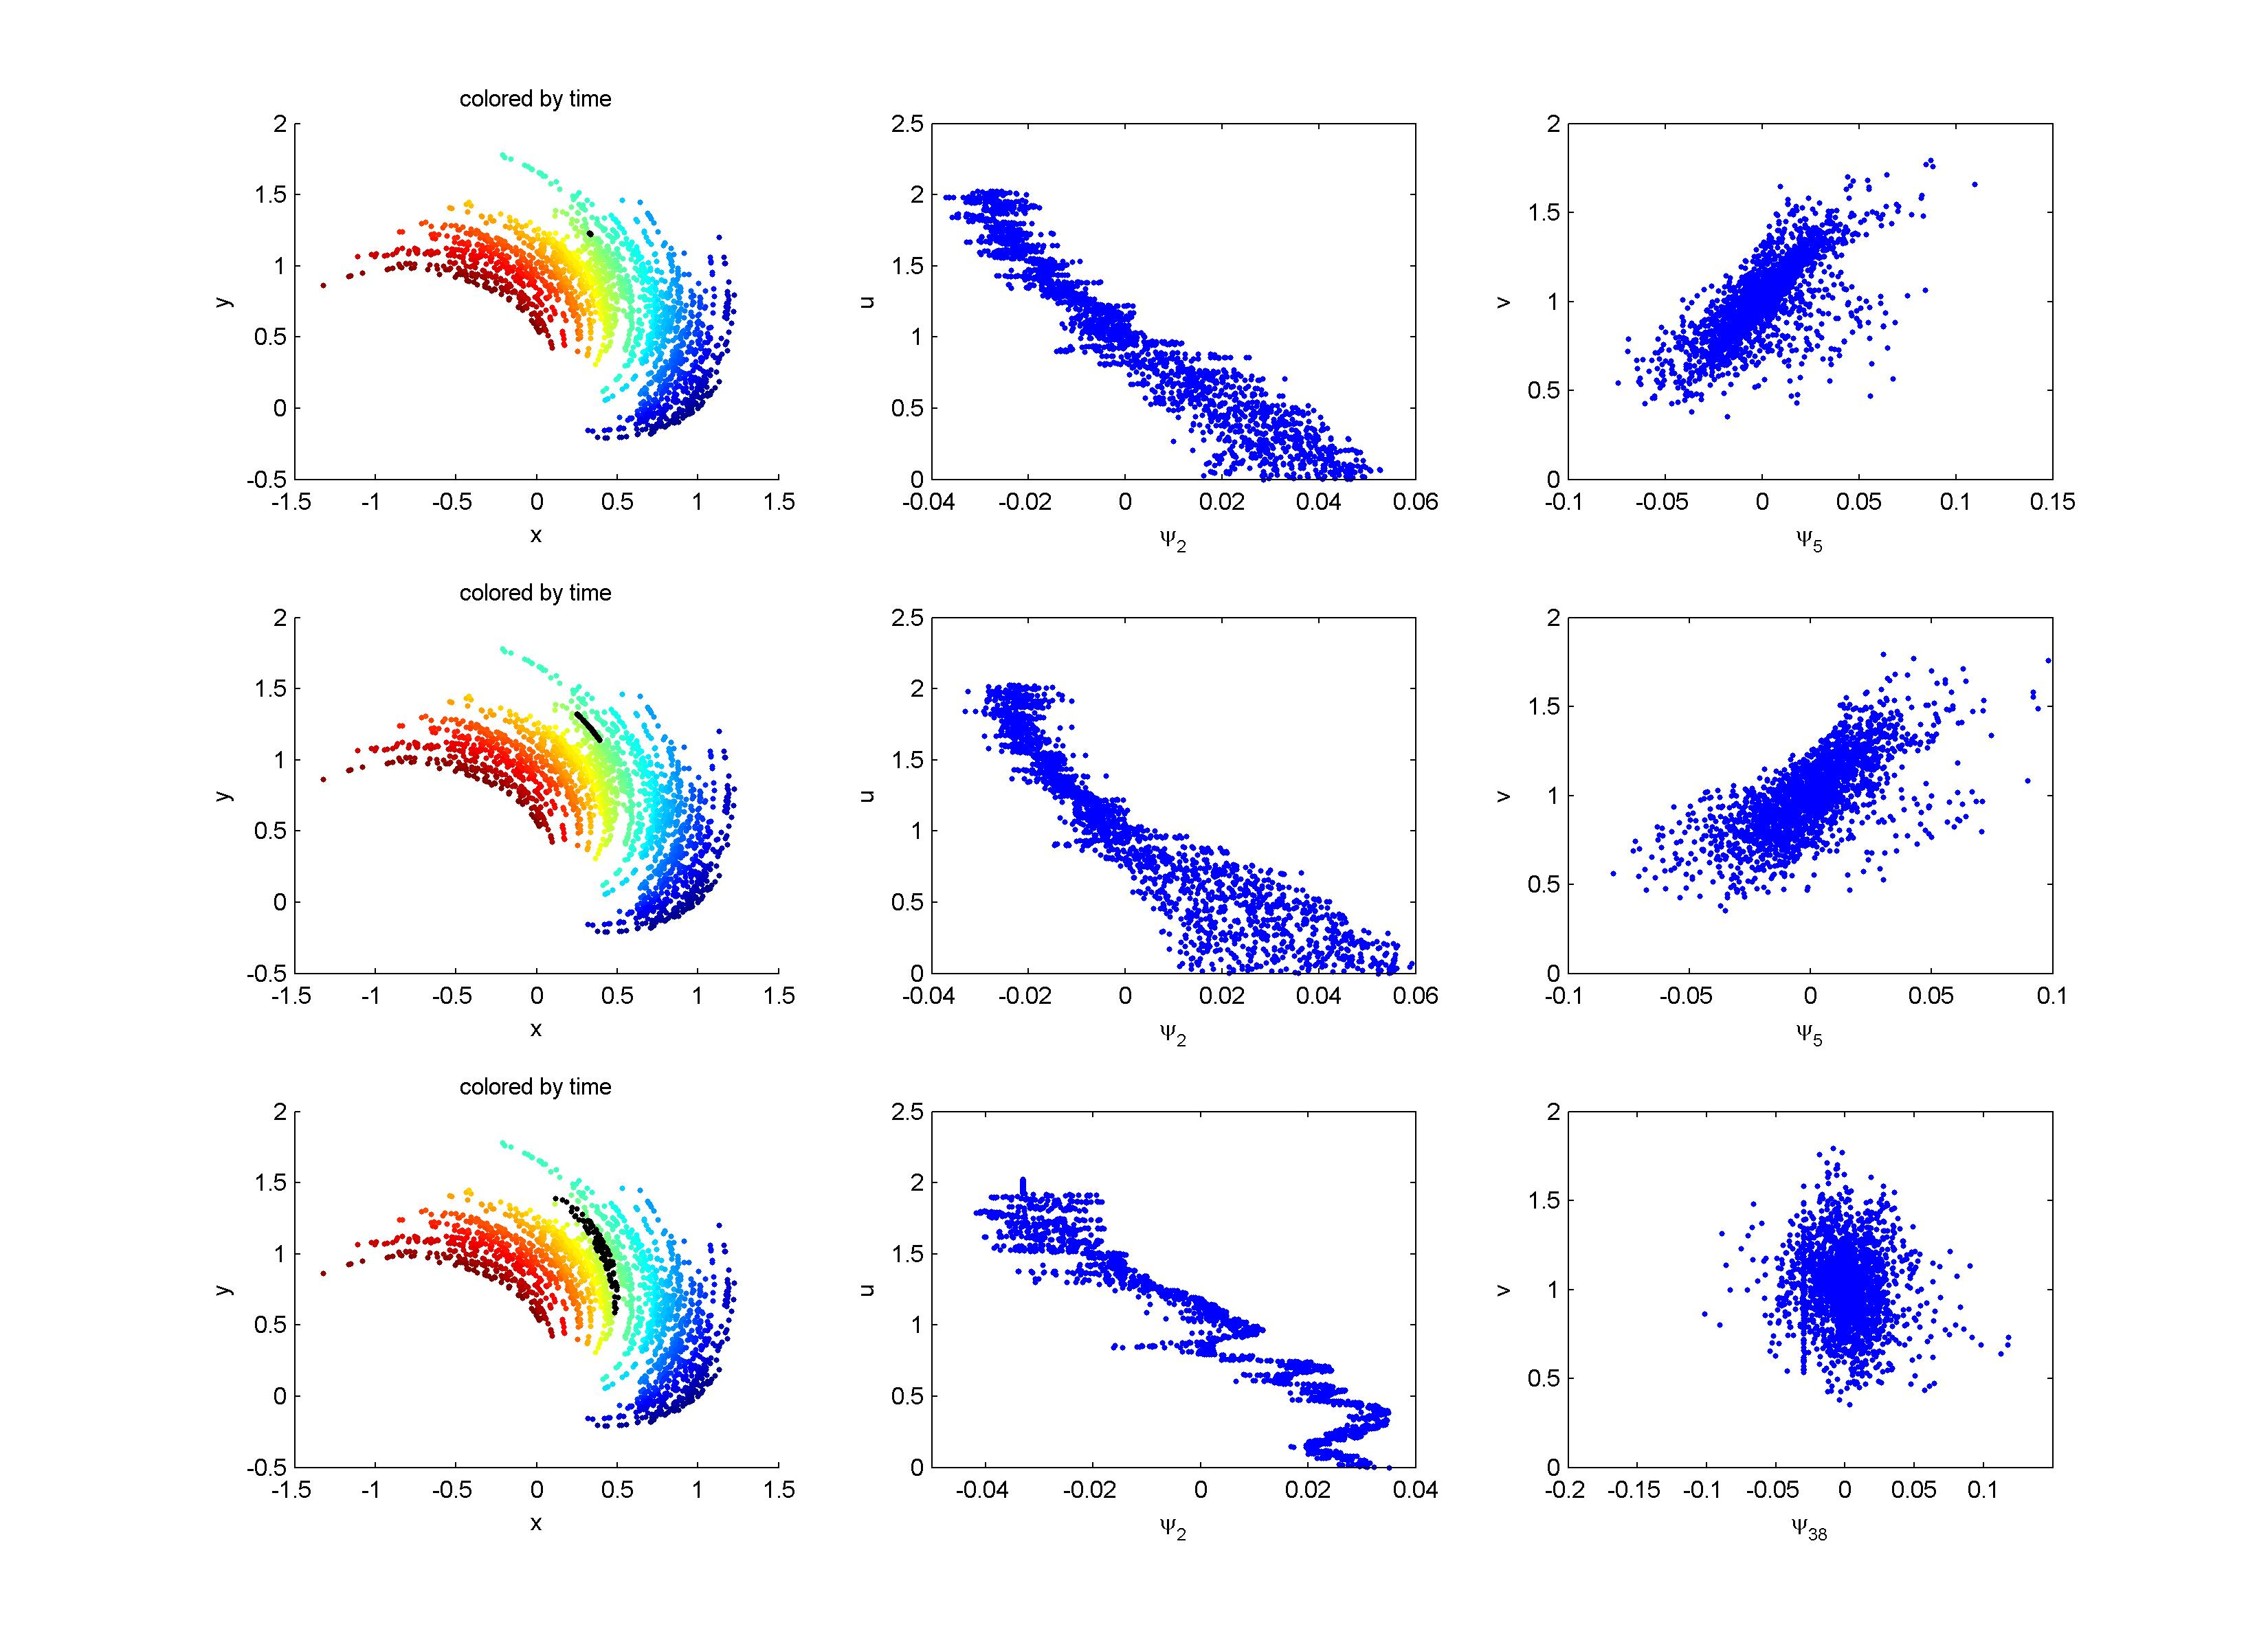
\includegraphics[width=\textwidth]{vary_windows_halfmoons}
\caption{Varying sampling windows with half moons. We can always recover the slow variable; only when the windows are smaller than the equilibrium measure of the fast do we also recover the fast variable. test\_half\_moons.m}
\label{fig:halfmoons}
\end{figure}



\section{Recovering NIVs}


Assume we have the following underlying dynamical system (two--dimensional Brownian motion)
\begin{eqnarray}
	dx_1 & = & a(x_1) dt + dW_1 \\
	dx_2 & = & a(x_2) dt + dW_2
\end{eqnarray}
where $a(x) = -100x^{99}$, $W_1, W_2$ are independent Browinain motions.
%
INstead of imposing reflective boundary conditons (like in the NLICA paper), $a$ is a potential that is very shallow in $[-1, 1]$, and very steep outside of this interval.
%
Therefore, we (effective) sample a square when simulating this SDE.
%
We then shift $x$
\begin{equation}
x \mapsto (x-1)/2
\end{equation}

We then apply following nonlinear transformation
%
\begin{eqnarray}
y_1 & = & x_1 + x_2^3 \\
y_2 & = & x_2 - x_1^3
\end{eqnarray}
%
The data are shown in Figure \ref{fig:data}.
%
TODO: change the figure so that it has the new data (SDE with shallow potential rather than Brownian motion with reflective bc)

\begin{figure}[htb]
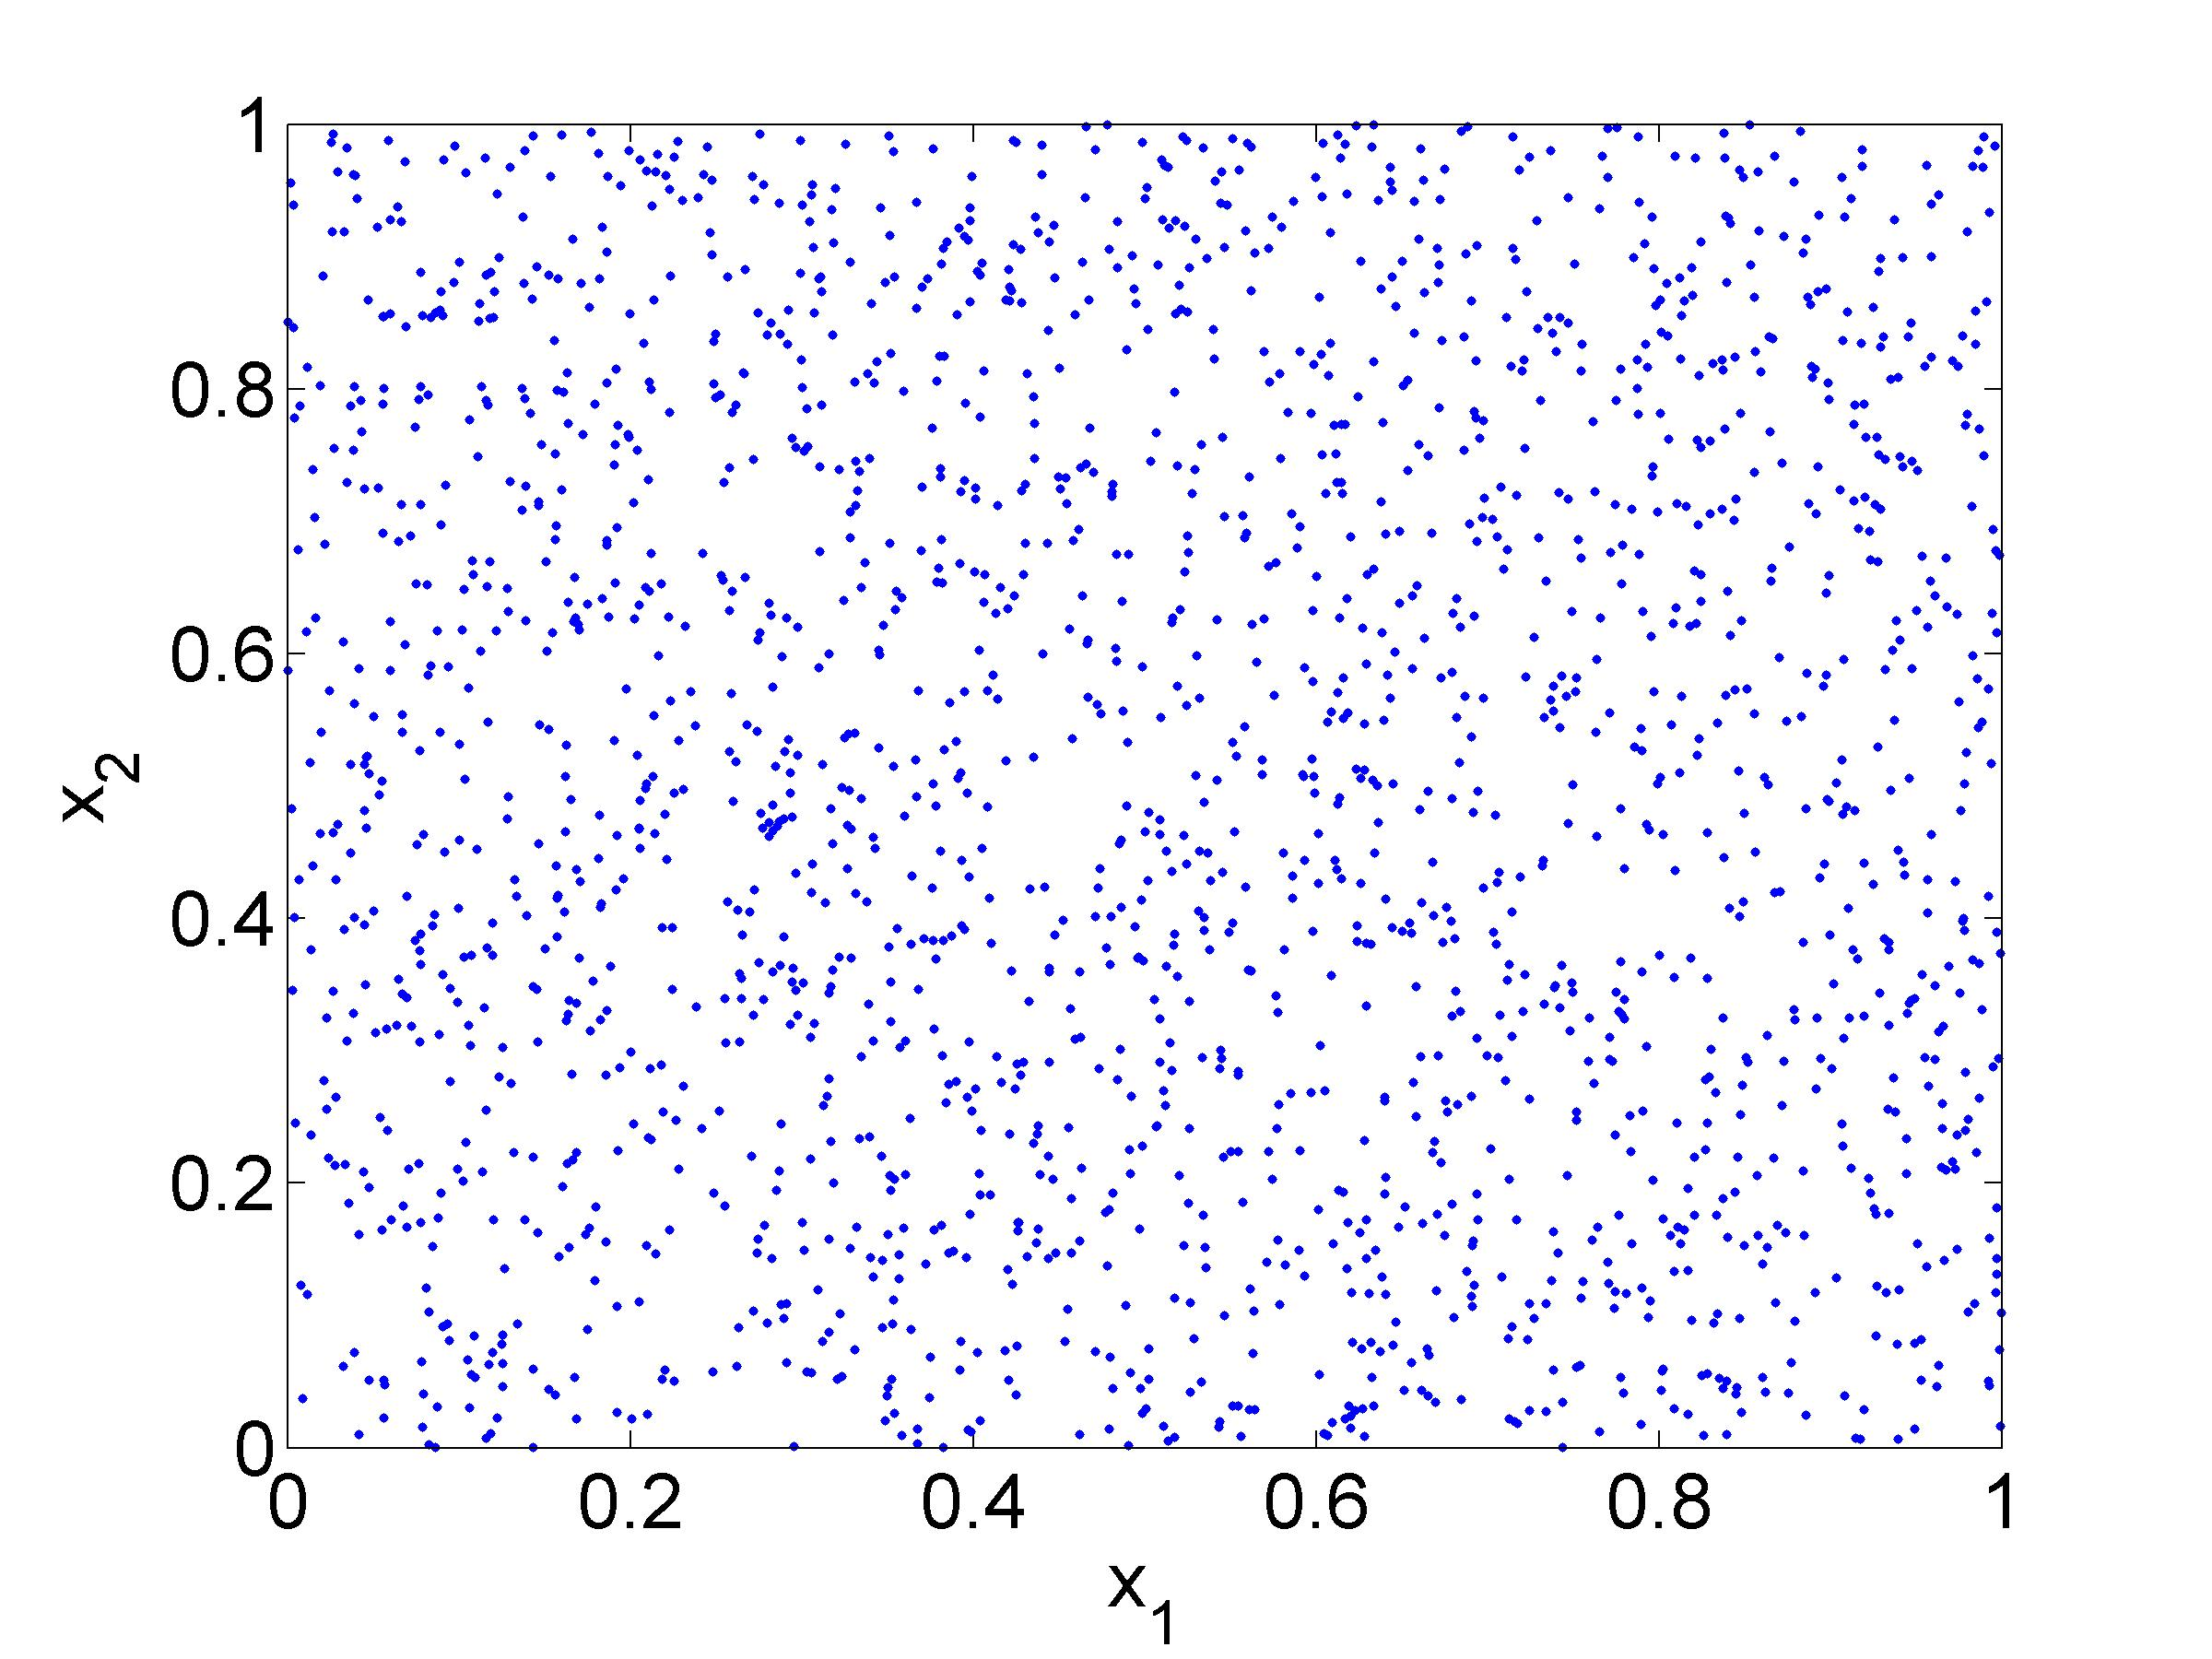
\includegraphics[width=0.5\textwidth]{xdata}
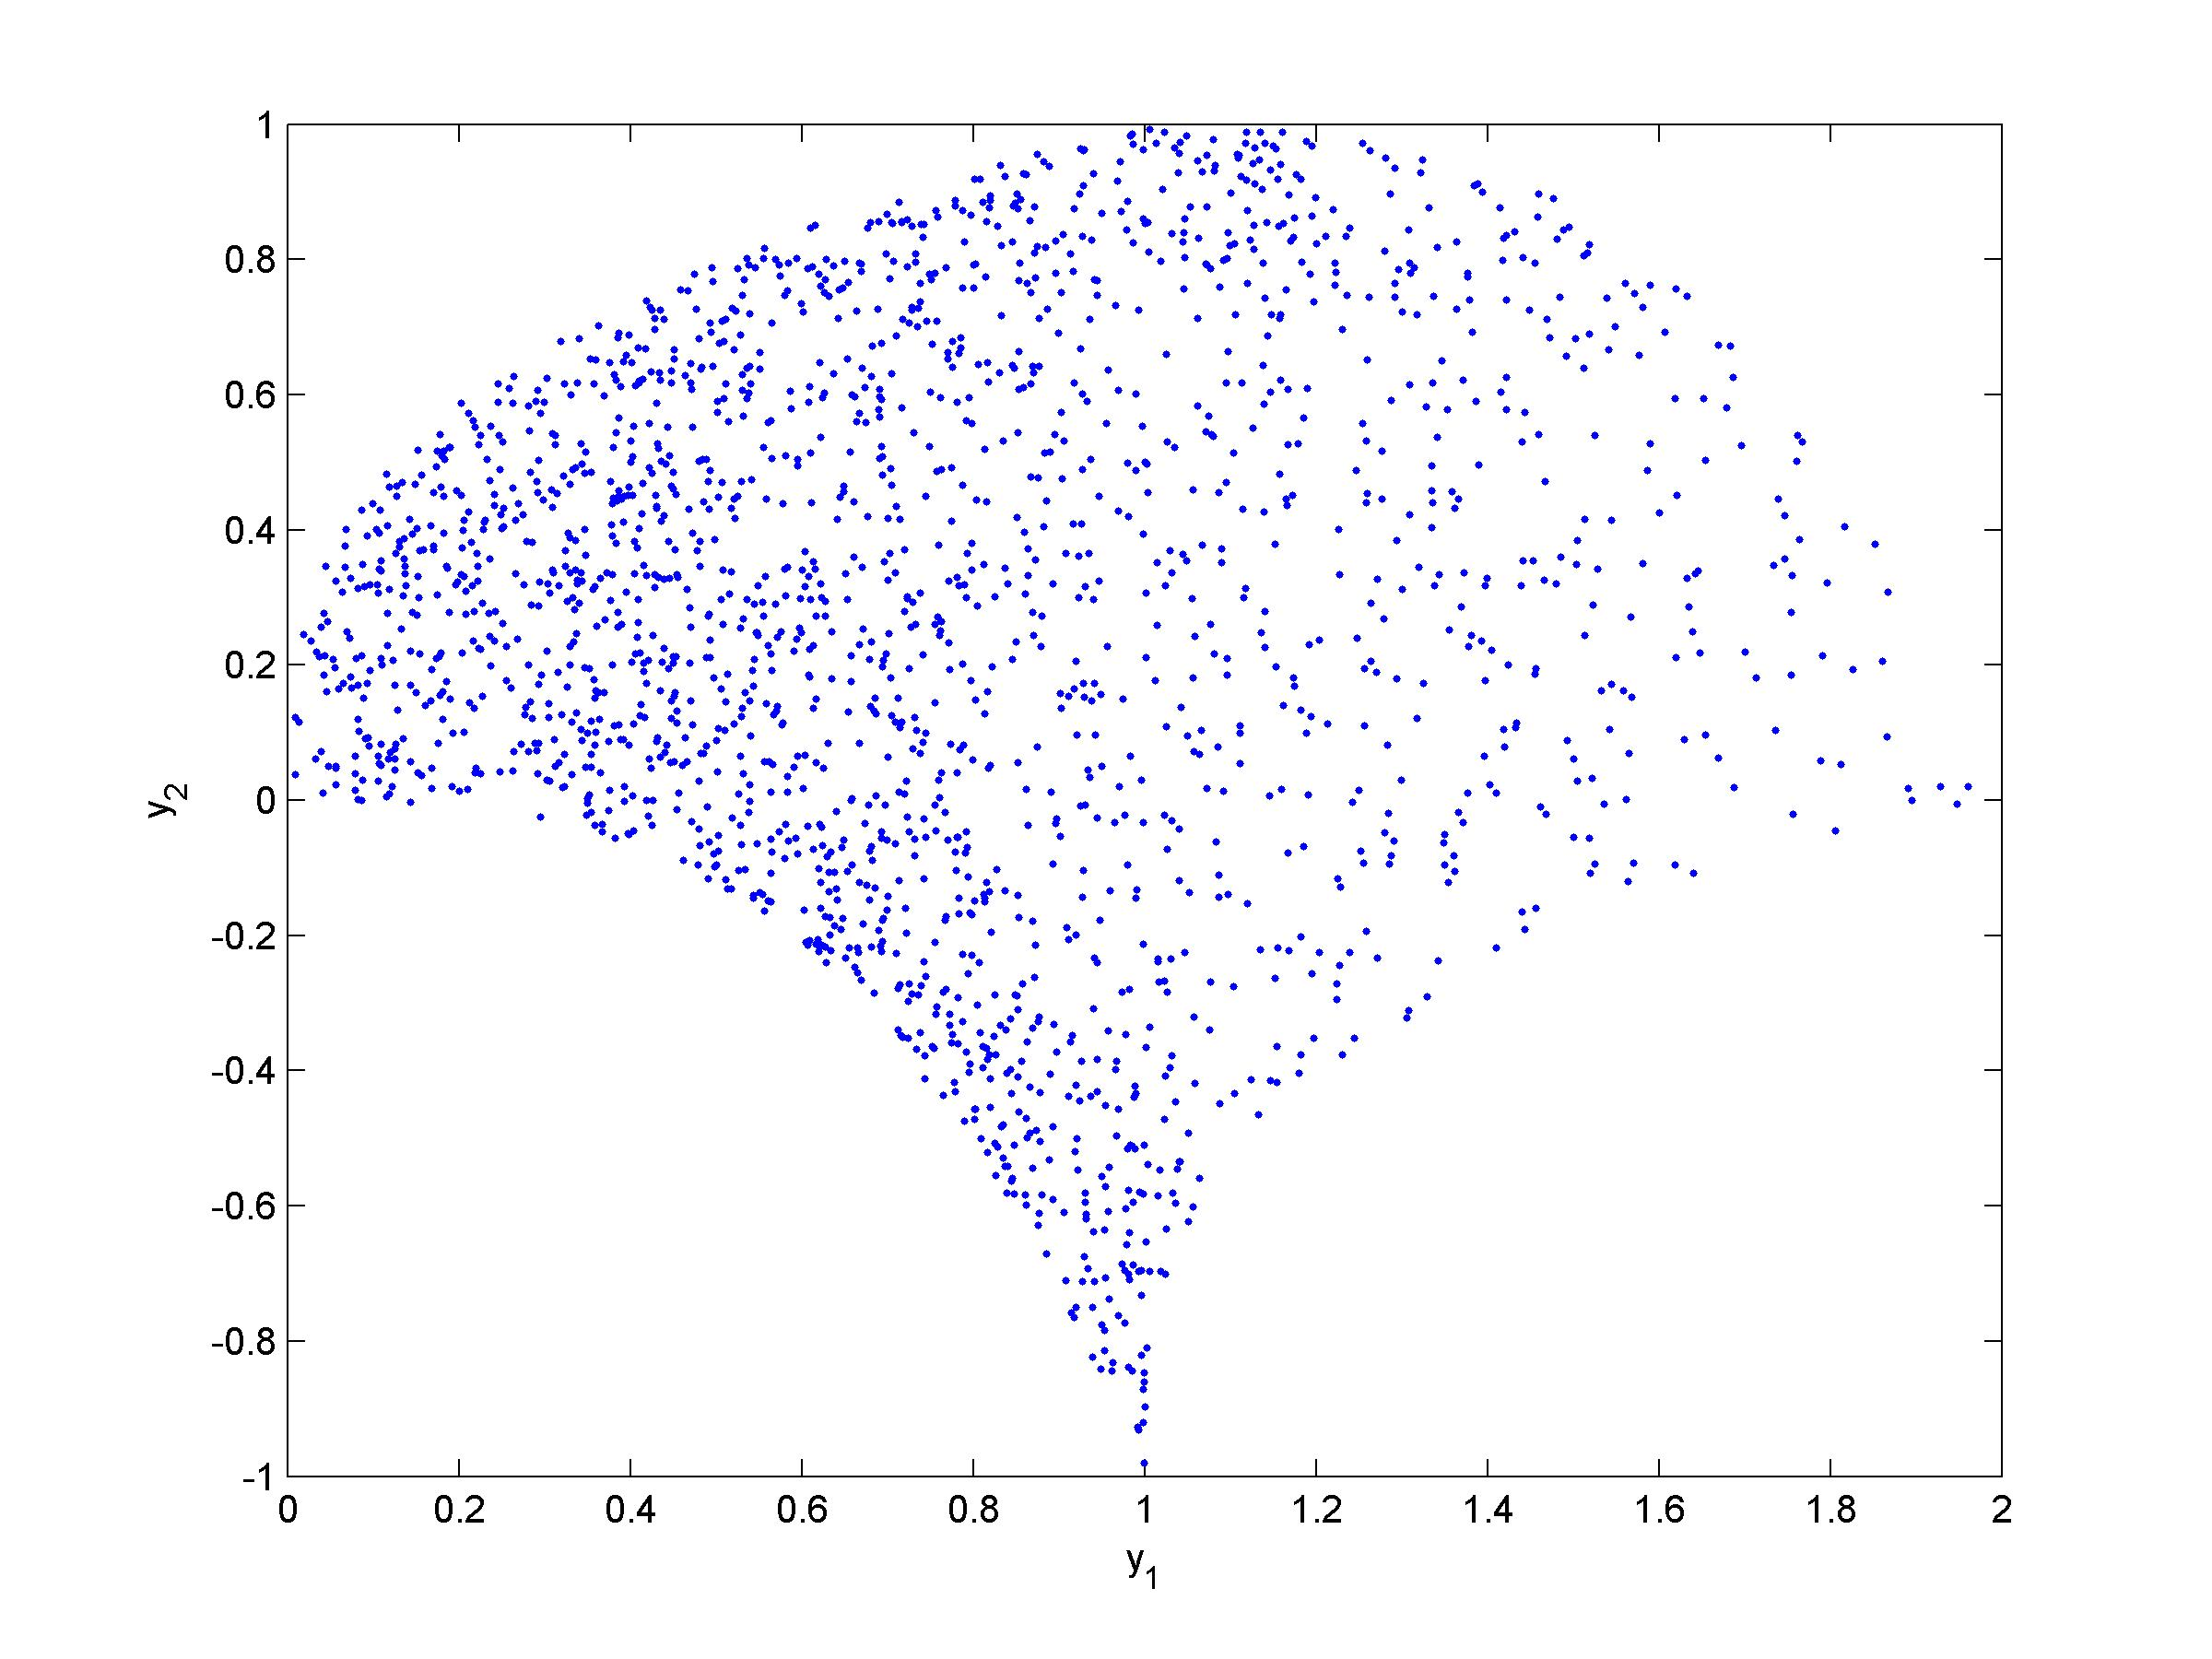
\includegraphics[width=0.5\textwidth]{ydata}
\caption{Left: data in ``intrinsic variable'' space ($x_1, x_2$). Right: data in ``ambient'' space ($y_1, y_2$).}
\label{fig:data}
\end{figure}

The DMAPS embedding computed from $y_1, y_2$ are shown in in Figure \ref{fig:xdata_dmaps}.
%
Note that we do not recover the ``correct'' parameterization of the underlying variables $x_1, x_2$.

\begin{figure}[H]
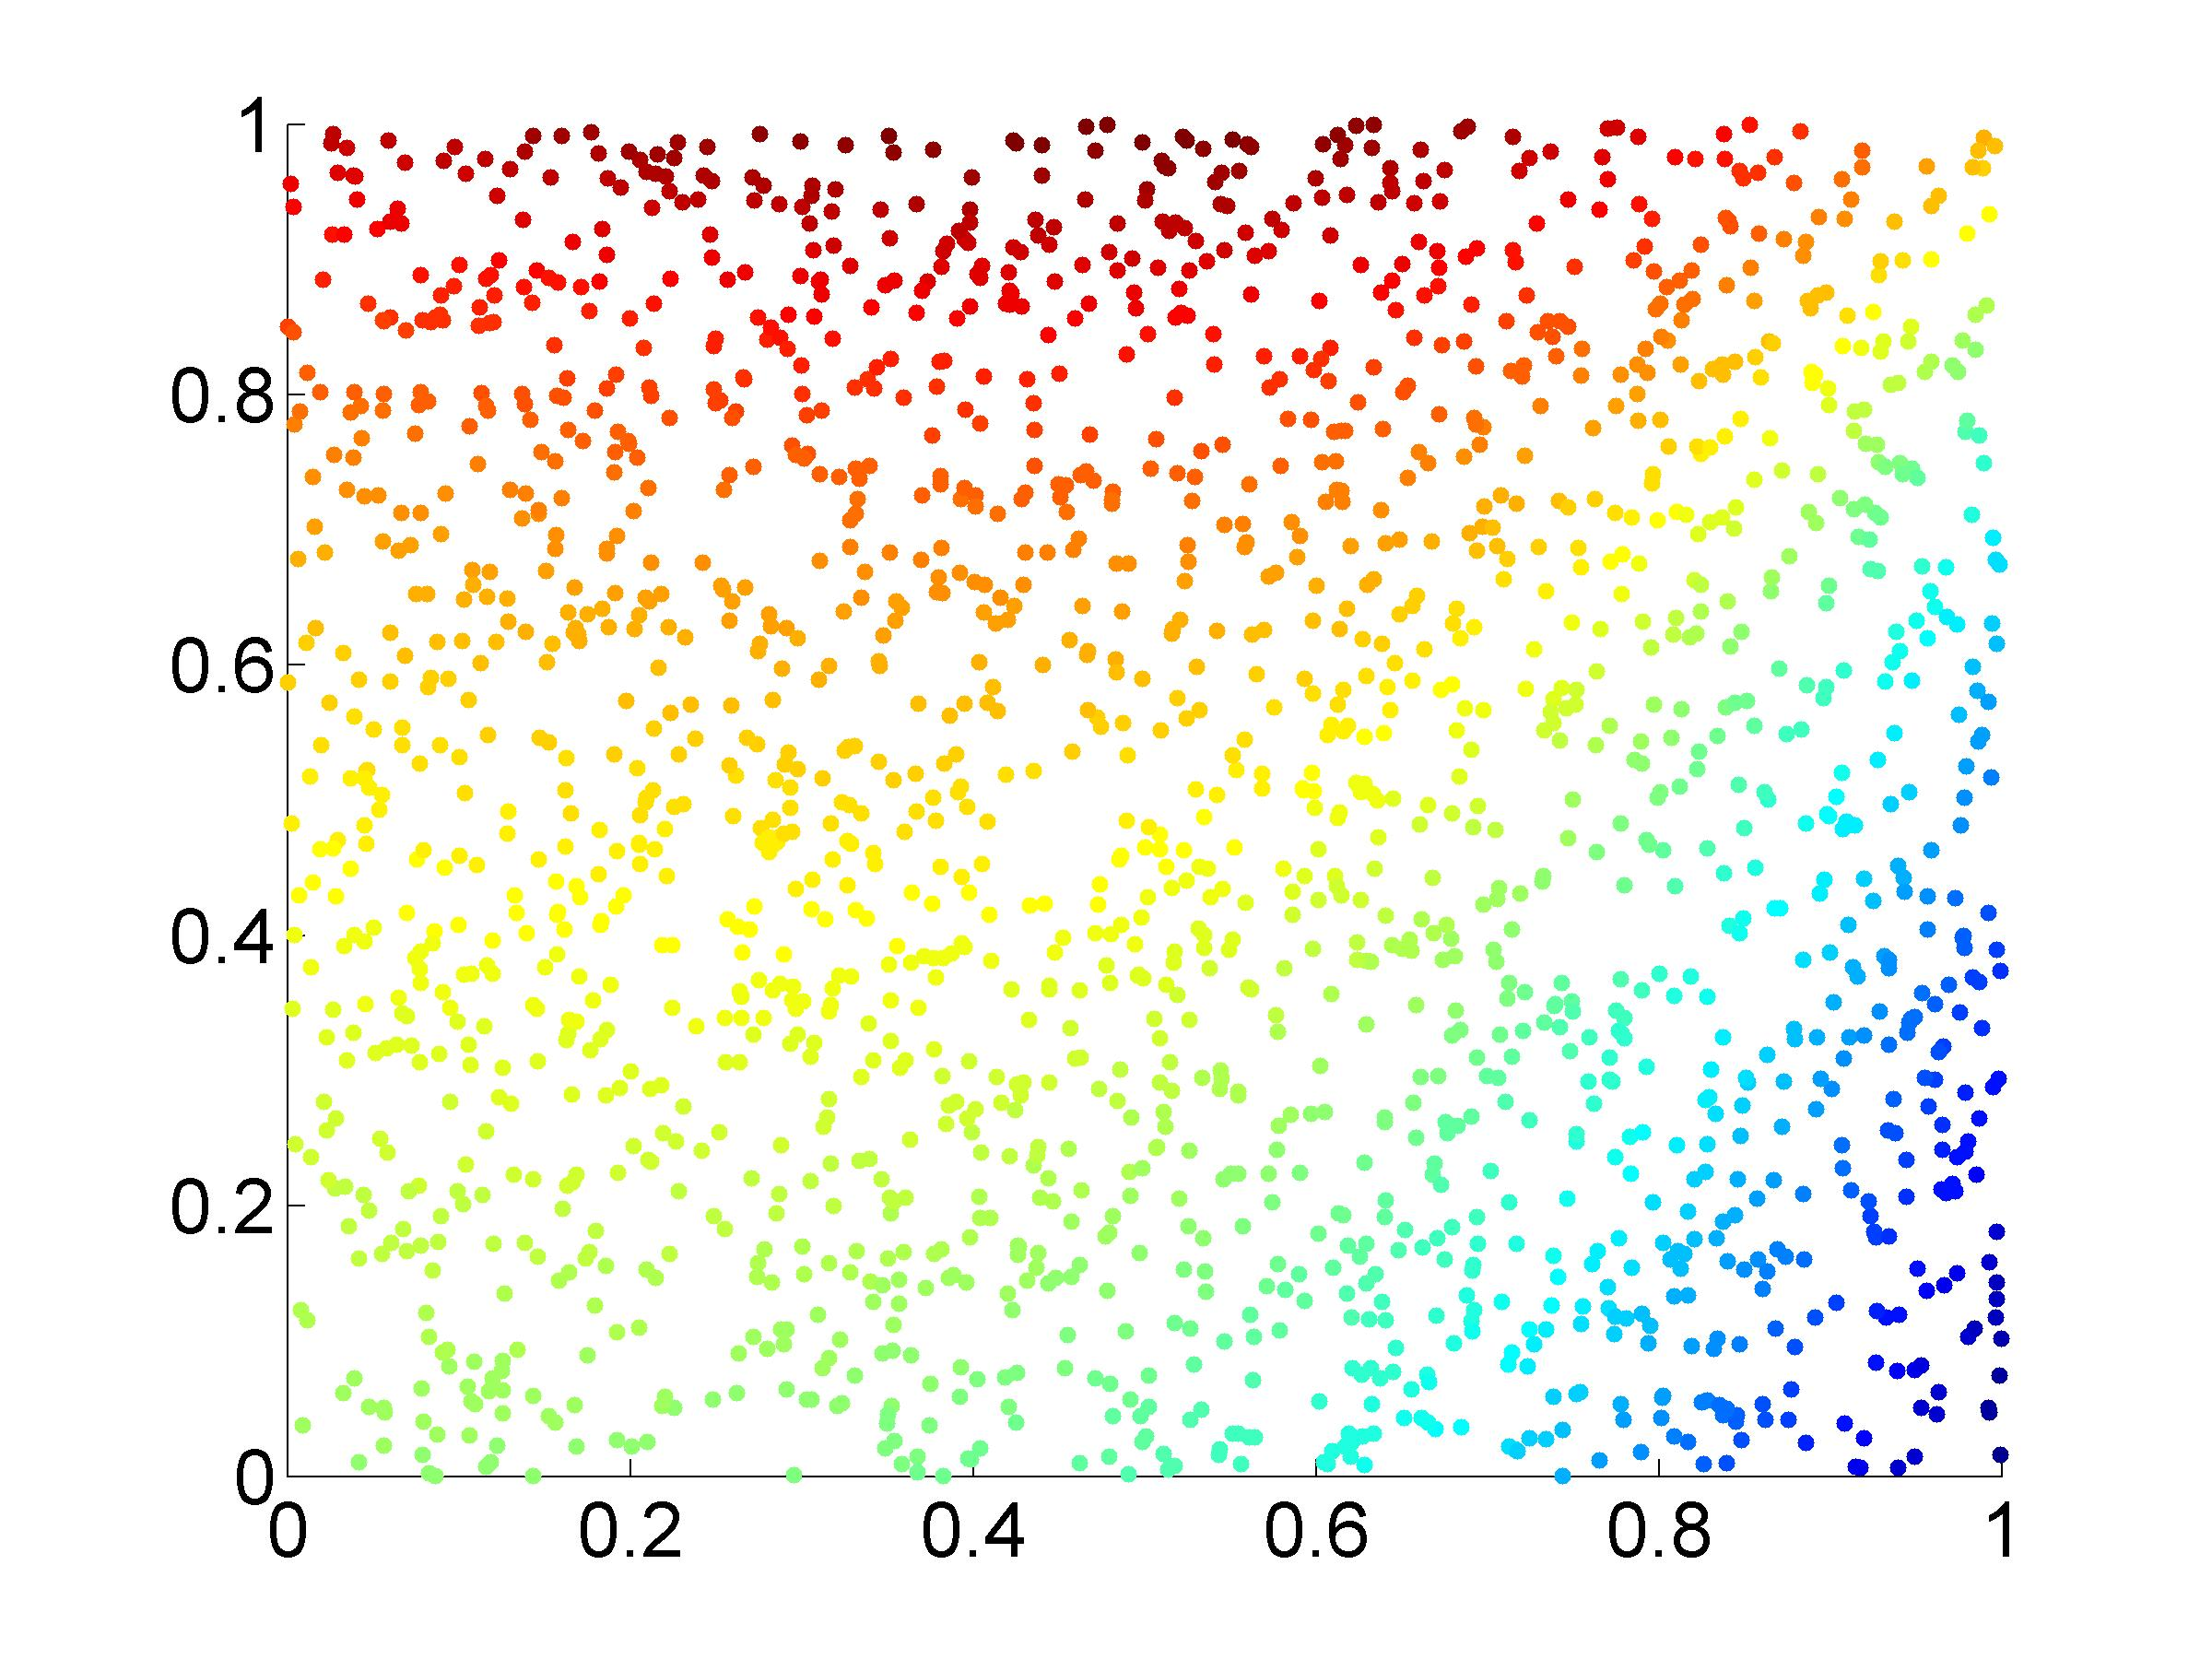
\includegraphics[width=0.3\textwidth]{xdata_colored_DMAPS1}
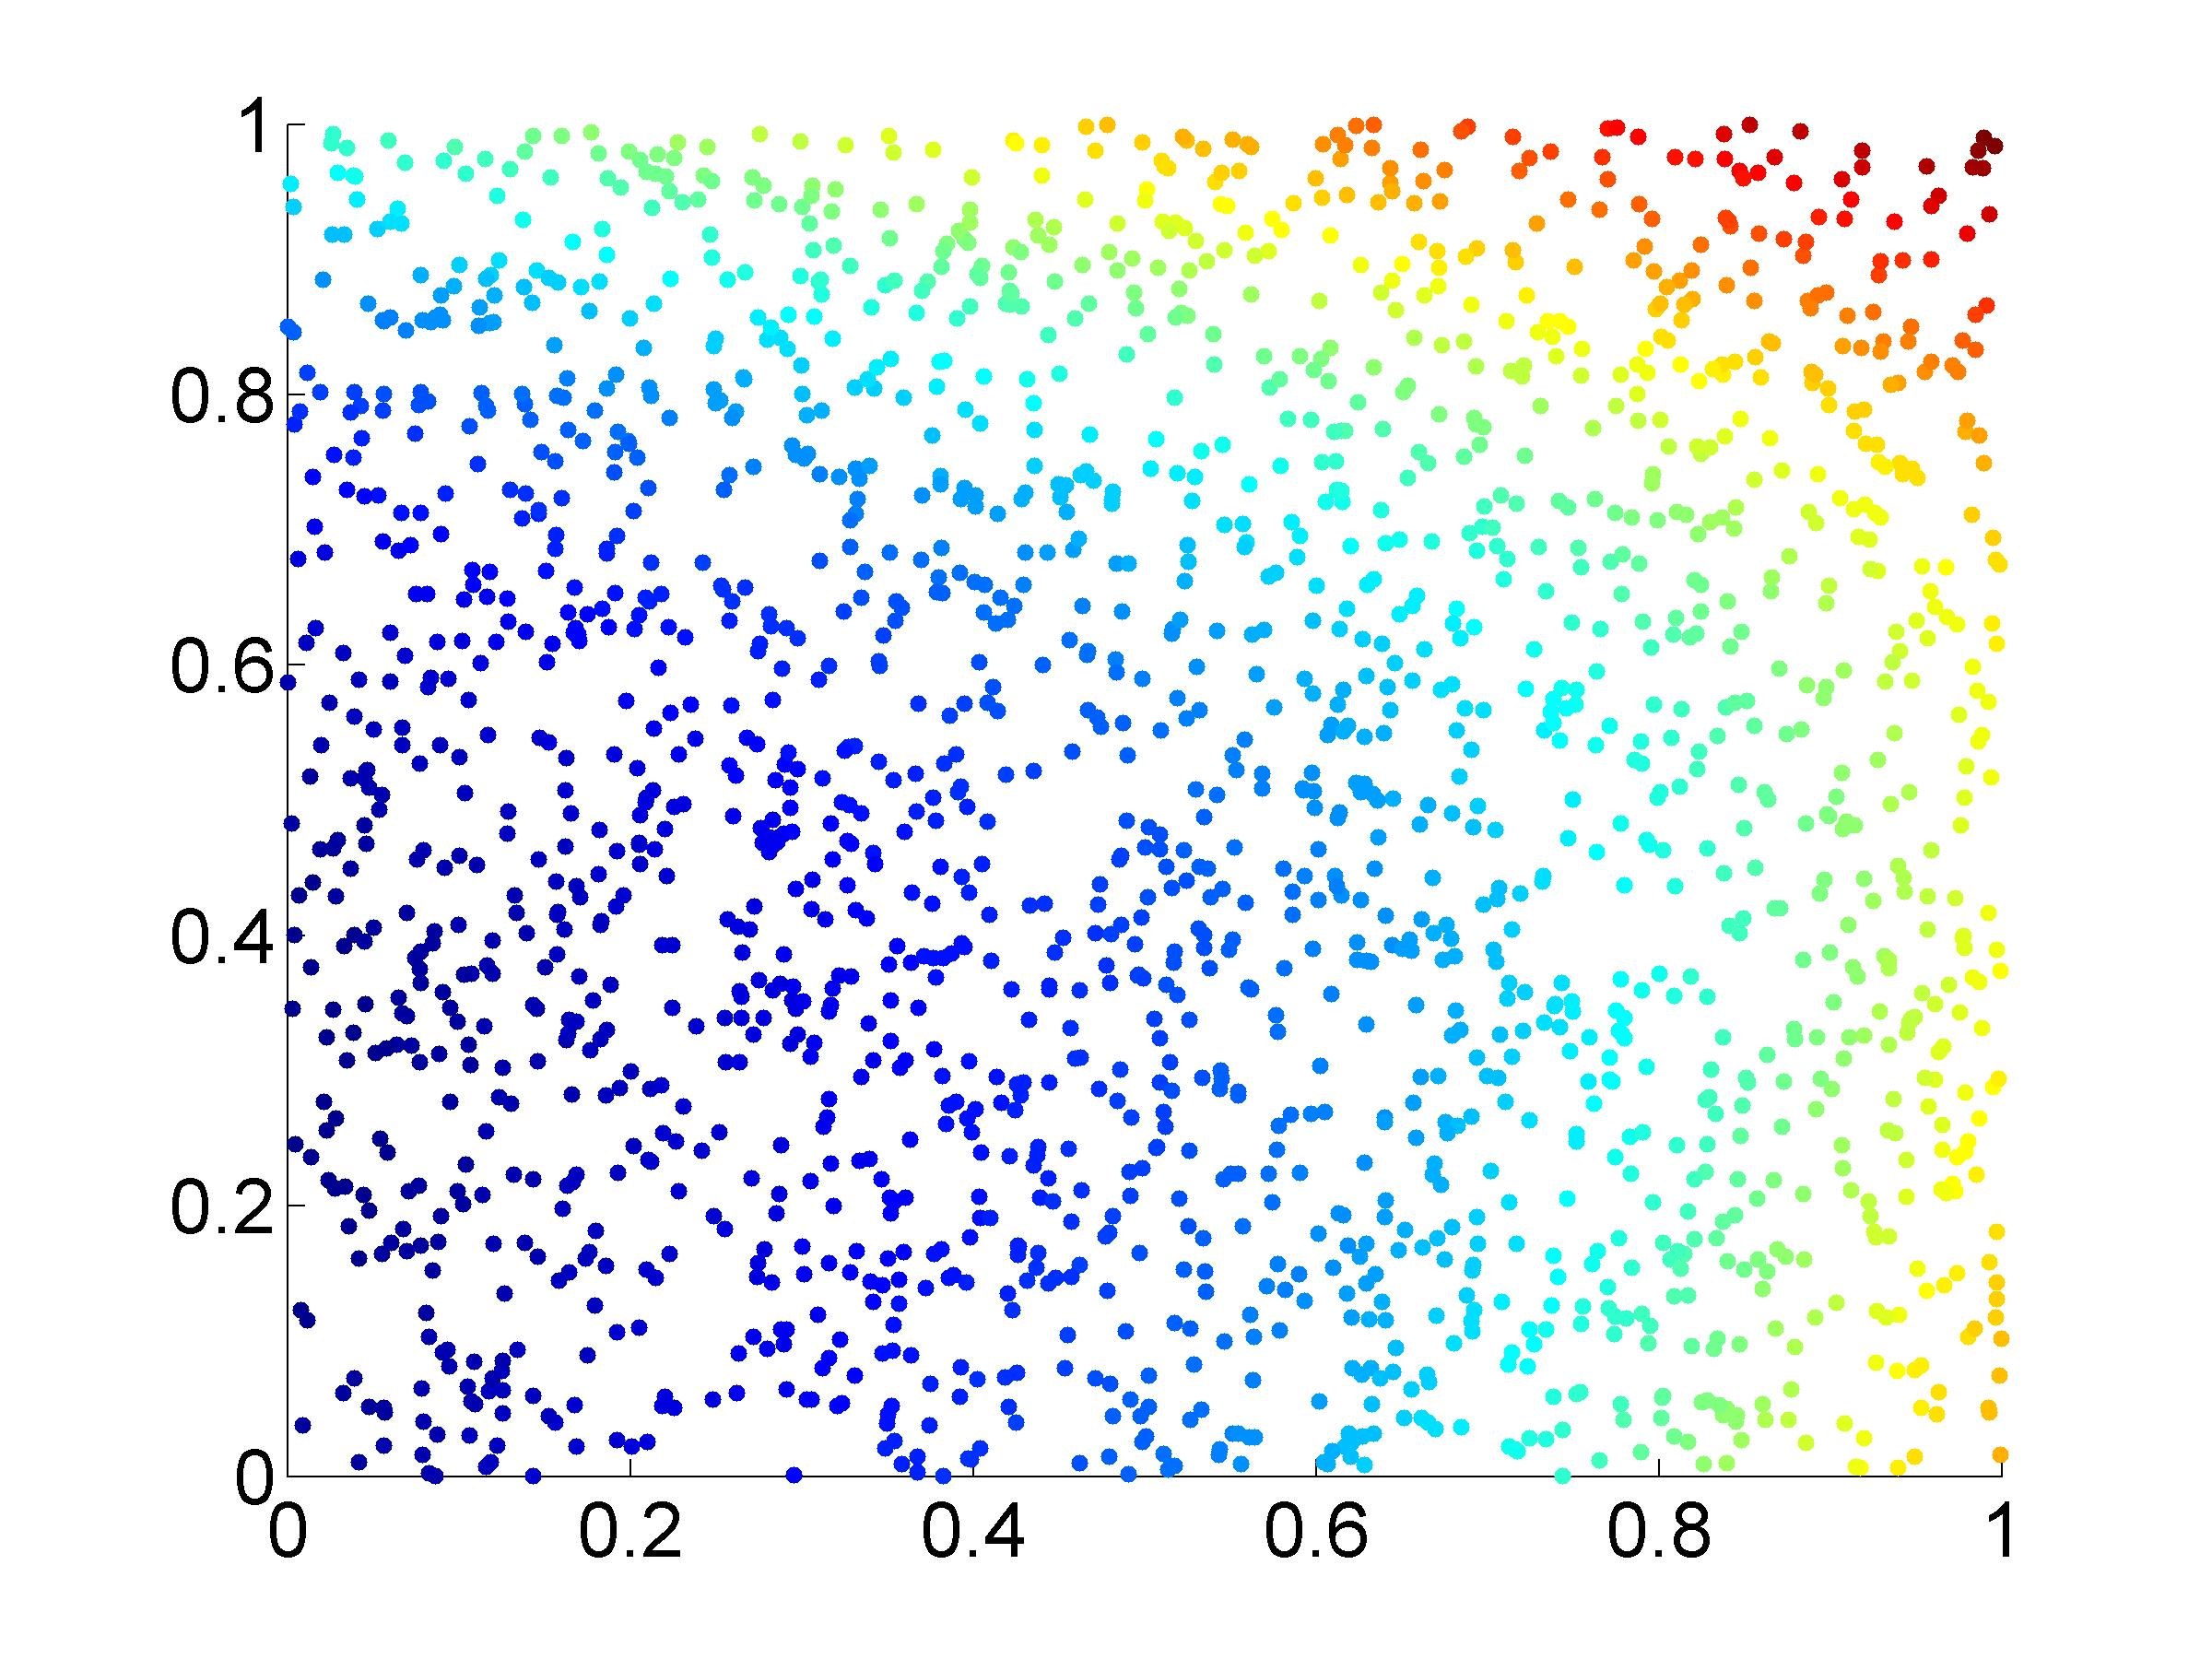
\includegraphics[width=0.3\textwidth]{xdata_colored_DMAPS2}
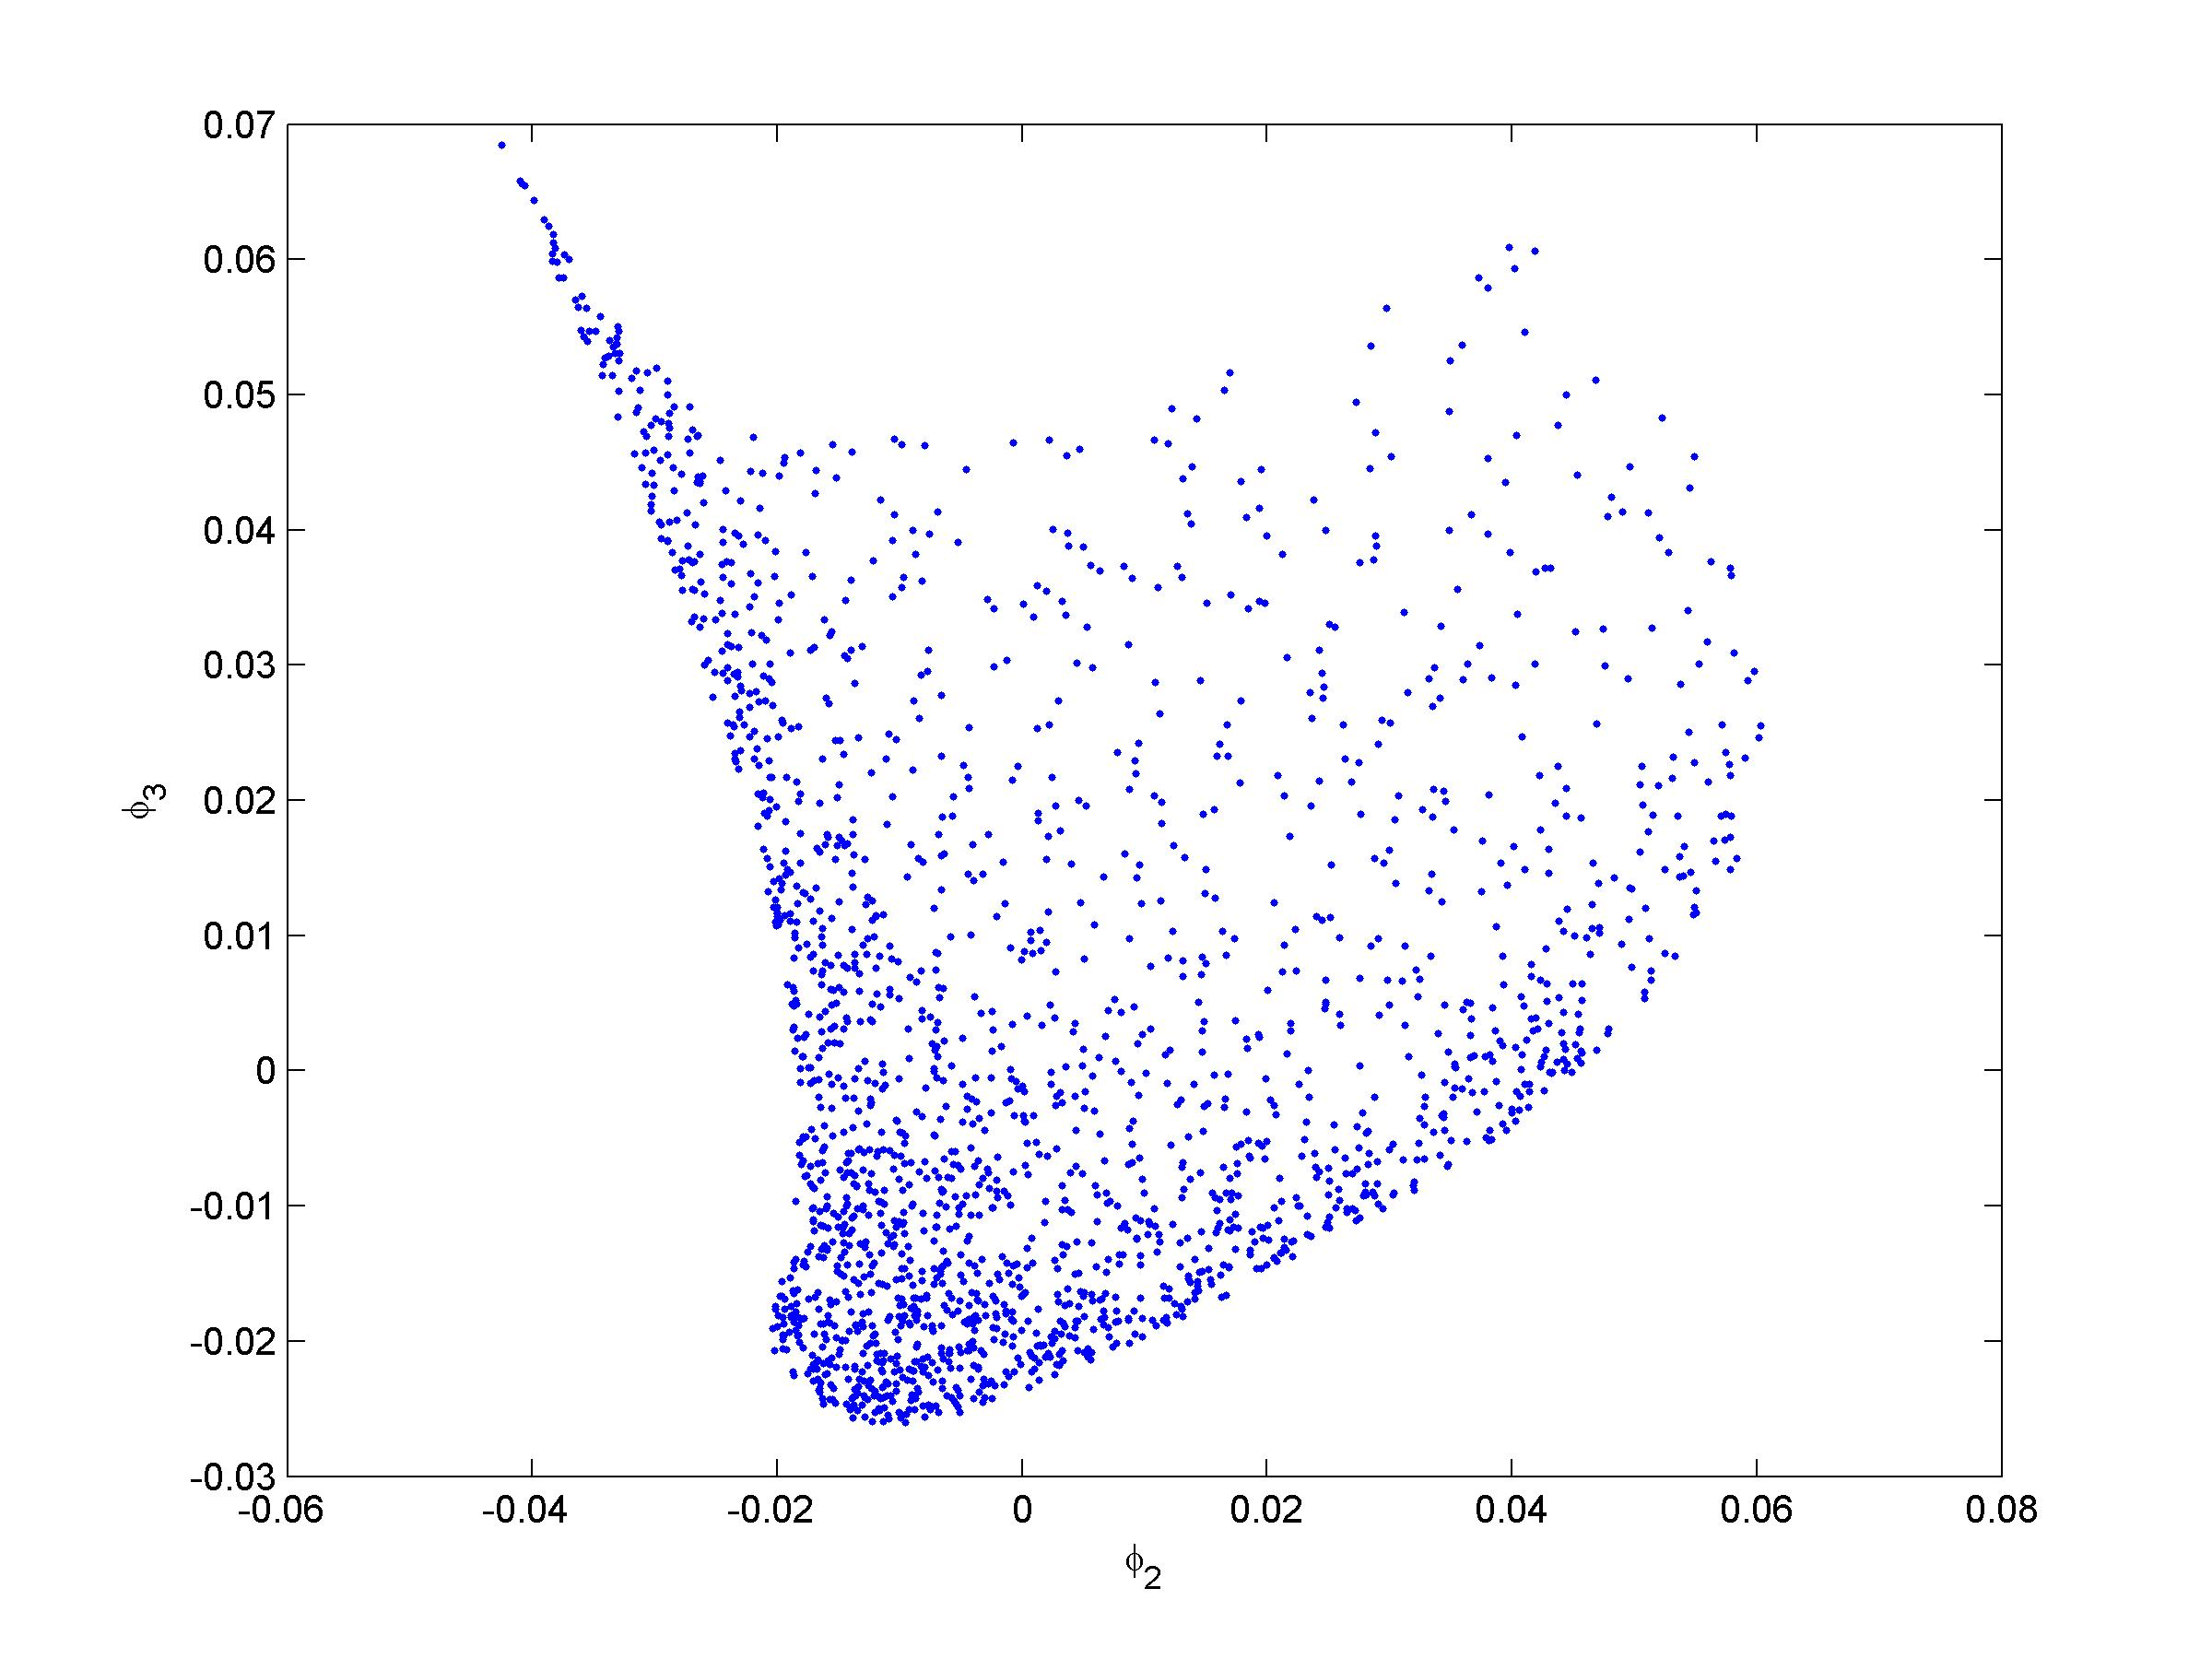
\includegraphics[width=0.3\textwidth]{embedding_dmaps}
\caption{Data in ``intrinsic variable'' space ($x_1, x_2$), colored by the first (left) and second (center) nontrivial DMAPS component. The DMAPS embedding is computed from the data in the ``ambient'' space ($y_1, y_2$). Note that the parameterizationa we obtain are not the eigenfunctions that we expect for points sampled from the unit square. (Right) Data plotted in first two (nontrivial) DMAPS variables.}
\label{fig:xdata_dmaps}
\end{figure}

The NIV embedding computed from $y_1, y_2$ are shown in in Figure  \ref{fig:xdata_NIV}.
%
Note that we now recover the ``correct'' variables.
%
TODO: we need to do this with covariance estimates from time series, rather than short busts. We need to also add the comparison between the analytical covariacne and the estimated covariances (based on differences from a single trajectory and also on bursts). 

\begin{figure}[H]
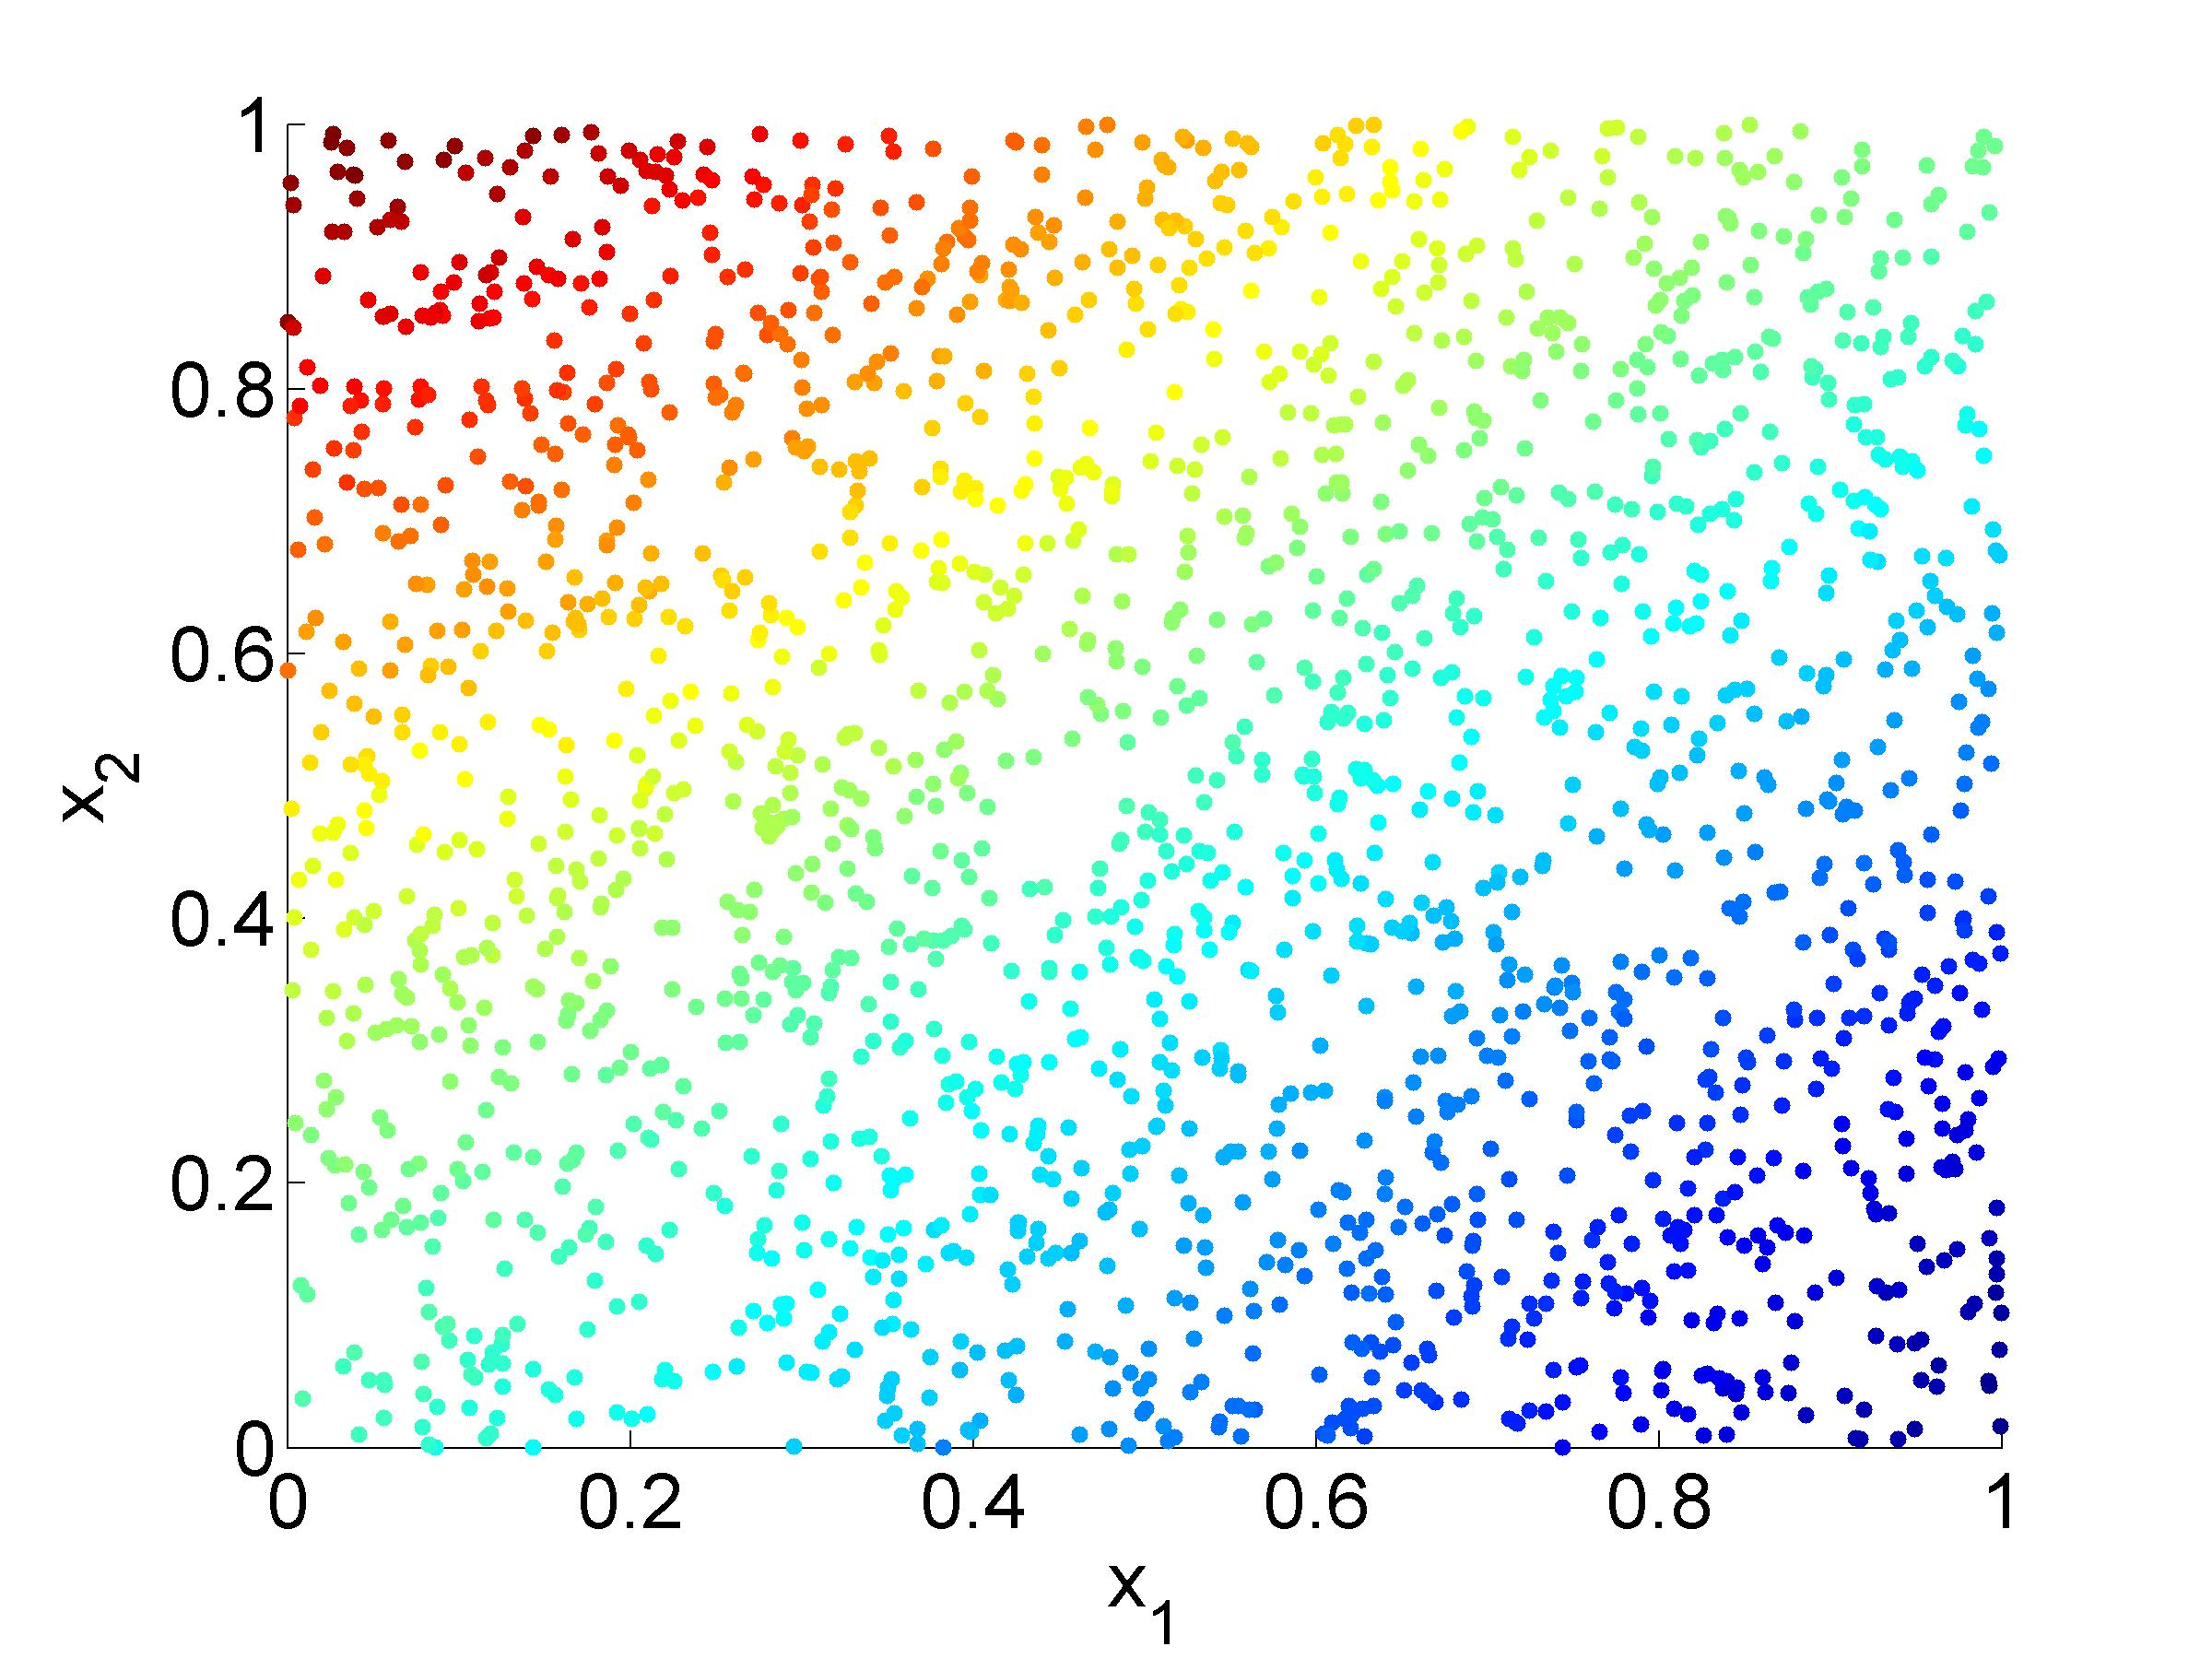
\includegraphics[width=0.3\textwidth]{xdata_colored_NIV1}
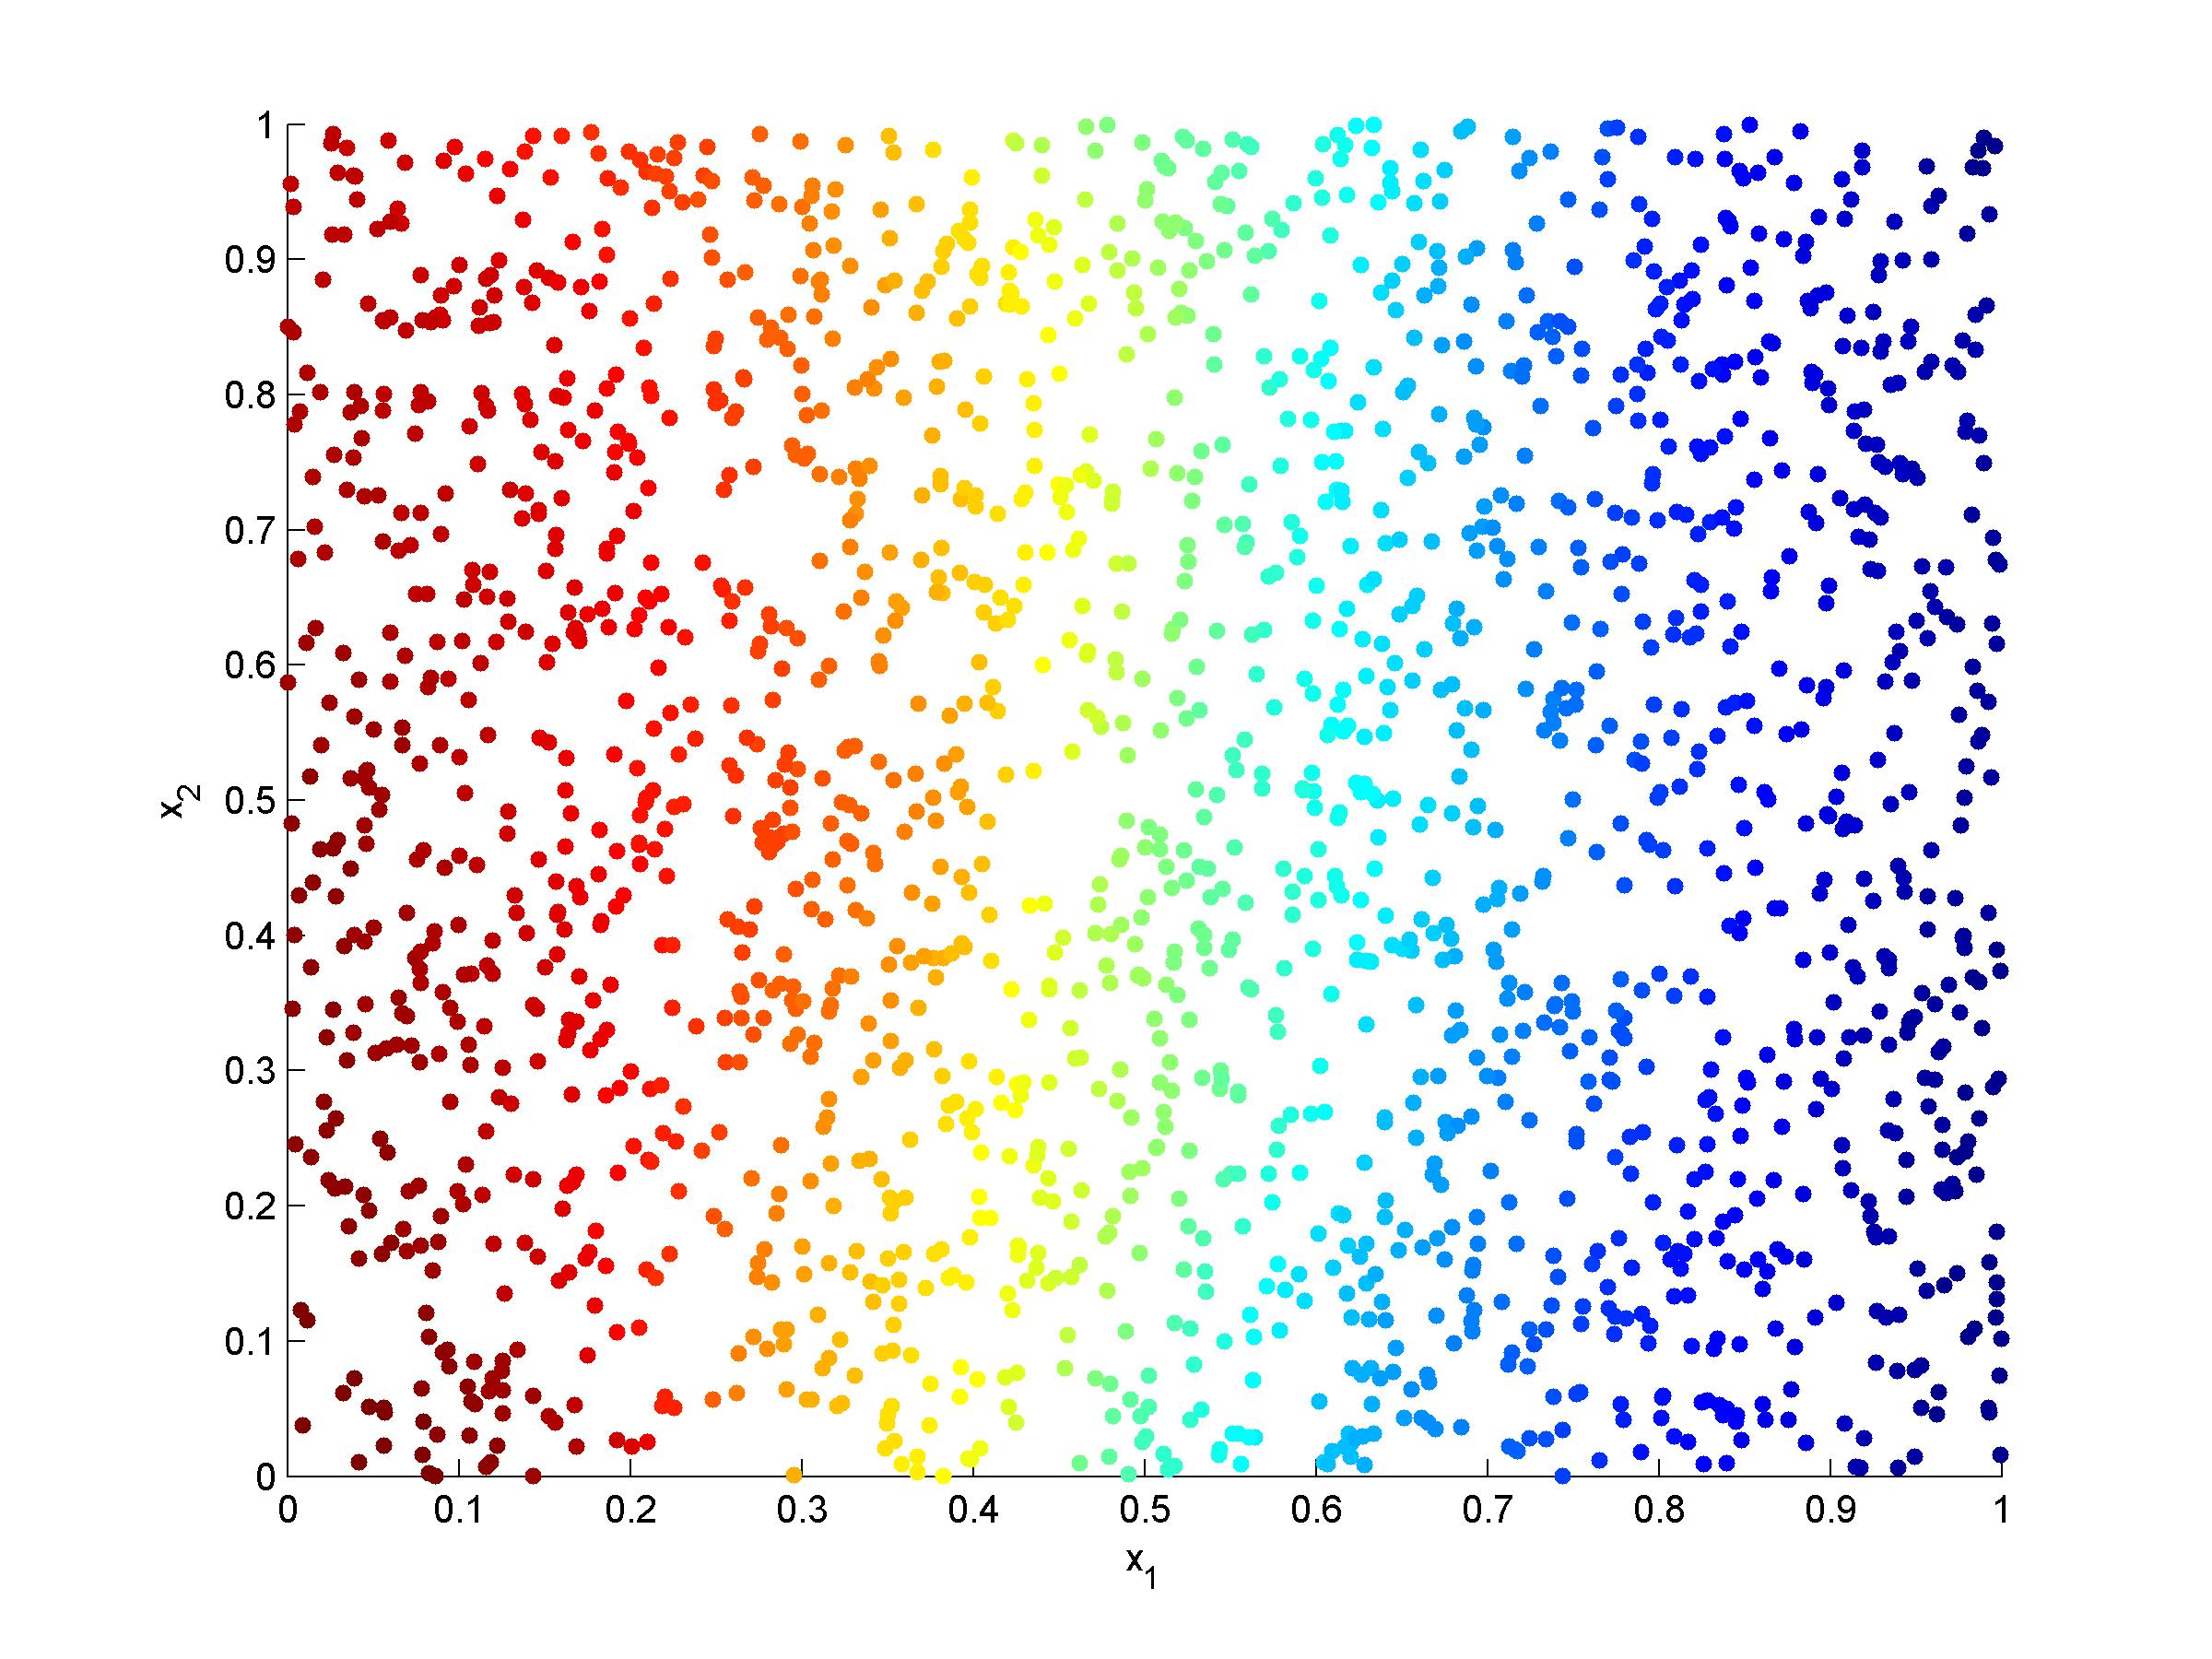
\includegraphics[width=0.3\textwidth]{xdata_colored_NIV2}
\includegraphics[width=0.3\textwidth]{embedding_NIV}
\caption{Data in ``intrinsic variable'' space ($x_1, x_2$), colored by the first (left) and second (center) nontrivial NIV. The NIV embedding is computed from the data in the ambient space ($y_1, y_2$), with time window $\Delta t = 0.01$. Note that the parameterizations we obtain are the eigenfunctions that we expect for points sampled from the unit square. (Right) Data plotted in first two (nontrivial) NIV.}
\label{fig:xdata_NIV}
\end{figure}

We now look at the effect of adding additional noise to our system.
%
Consider adding noise which saturates at some time scale
\begin{eqnarray}
z_1(t) & = & r\frac{x_1(t) + x_2(t)^3}{\sqrt{(x_1(t)+x_2(t)^3)^2 + (x_2(t)-x_1(t)^3)^2+1}} + \xi_1(t) \\
z_2(t) & = & r\frac{x_2(t) - x_1(t)^3}{\sqrt{(x_1(t)+x_2(t)^3)^2 + (x_2(t)-x_1(t)^3)^2+1}} + \xi_2(t) \\
z_3(t) & = & r\frac{1}{\sqrt{(x_1(t)+x_2(t)^3)^2 + (x_2(t)-x_1(t)^3)^2+1}} + \xi_3(t)
\end{eqnarray}
%
where $r$ is the radius of the sphere onto which we project, and
\begin{equation}
d \xi_i(\tau) = L a(\xi_i) d\tau + \frac{1}{\sqrt{\epsilon}} d\tilde{W}_i
\end{equation}
TODO: fix this to match the scaling in the code (scaled time and length). 

In conclusion, when this no longer works (when we cannot reover NIVs from a single application of Mahalanobis/NLICA), we need to introduce intermediate representations for our data that averages out the fast noise.

\begin{figure}[h!]
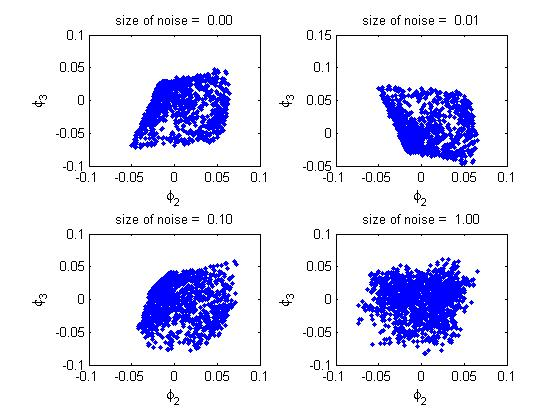
\includegraphics[width=0.5\textwidth]{embeddings_vary_with_noise_r1}
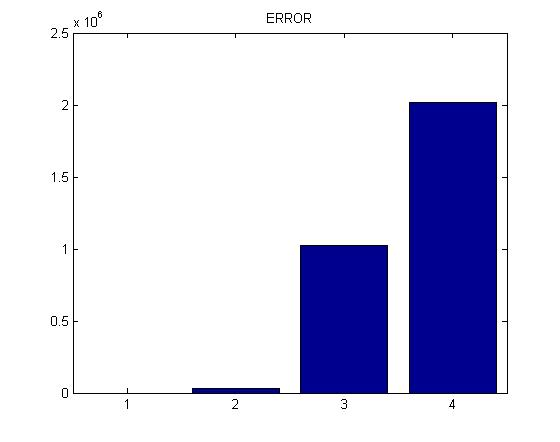
\includegraphics[width=0.5\textwidth]{error_with_noise}
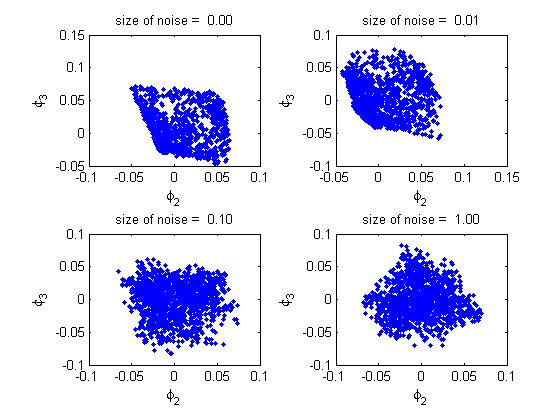
\includegraphics[width=0.5\textwidth]{embeddings_vary_with_noise_r01}
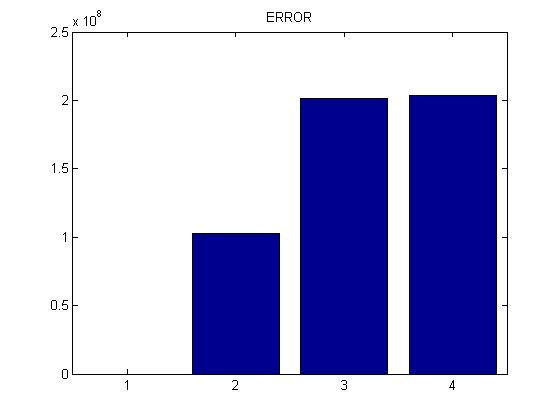
\includegraphics[width=0.5\textwidth]{error_with_noise_01}
\caption{Example from Amit's NLICA paper, section 6.2 (Mushroom on sphere). Top, left: sphere of radius $r=1$. Change scale of ambient noise. As ambient noise increases, the embedding becomes poorer, since the ambient noise hides the shape of the mushroom originated by the intrinsic noise. The scale of the intrinsic noise is 0.1. Top, right: Error in inverse covariances relative to the inverse covariances when there is no noise. We see where the embedding breaks down (corresponds to increase in the error). Bottom, left: same thing, for $r=0.1$. The embedding breaks down at a smaller size of noise, due to (1) the nonlinear transformation is more curved and the covariance estimation is less accurrate, and (2) the effective scale of the intrinsic noise is smaller. Bottom, right: Error in the inverse covariances. The embedding breaks down when the error increases substantially. TODO: Compare with the analytic covariance (maybe through the eigenvectors/singular vectors). test\_2d\_1d\_example.m}
\end{figure}


%If $\sigma = 0.01$ (so the added noise is much smaller than the noise in the original clouds), we obtain a parameterization shown in Figure \ref{fig:xdata_NIV_noise1} using NIV.
%%
%When we do NIV, the ``ellipses'' we see are a combination of the original noises in the intrinsic variables and the noise in the ambient space.
%%
%Because the noise in the ambient space is significantly smaller than the noise in the intrinsic variable space, we can still ``see'' the directions of the intrinsic variable noises in the ellipses, and therefore uncover the intrinsic variables.
%
%\begin{figure}[H]
%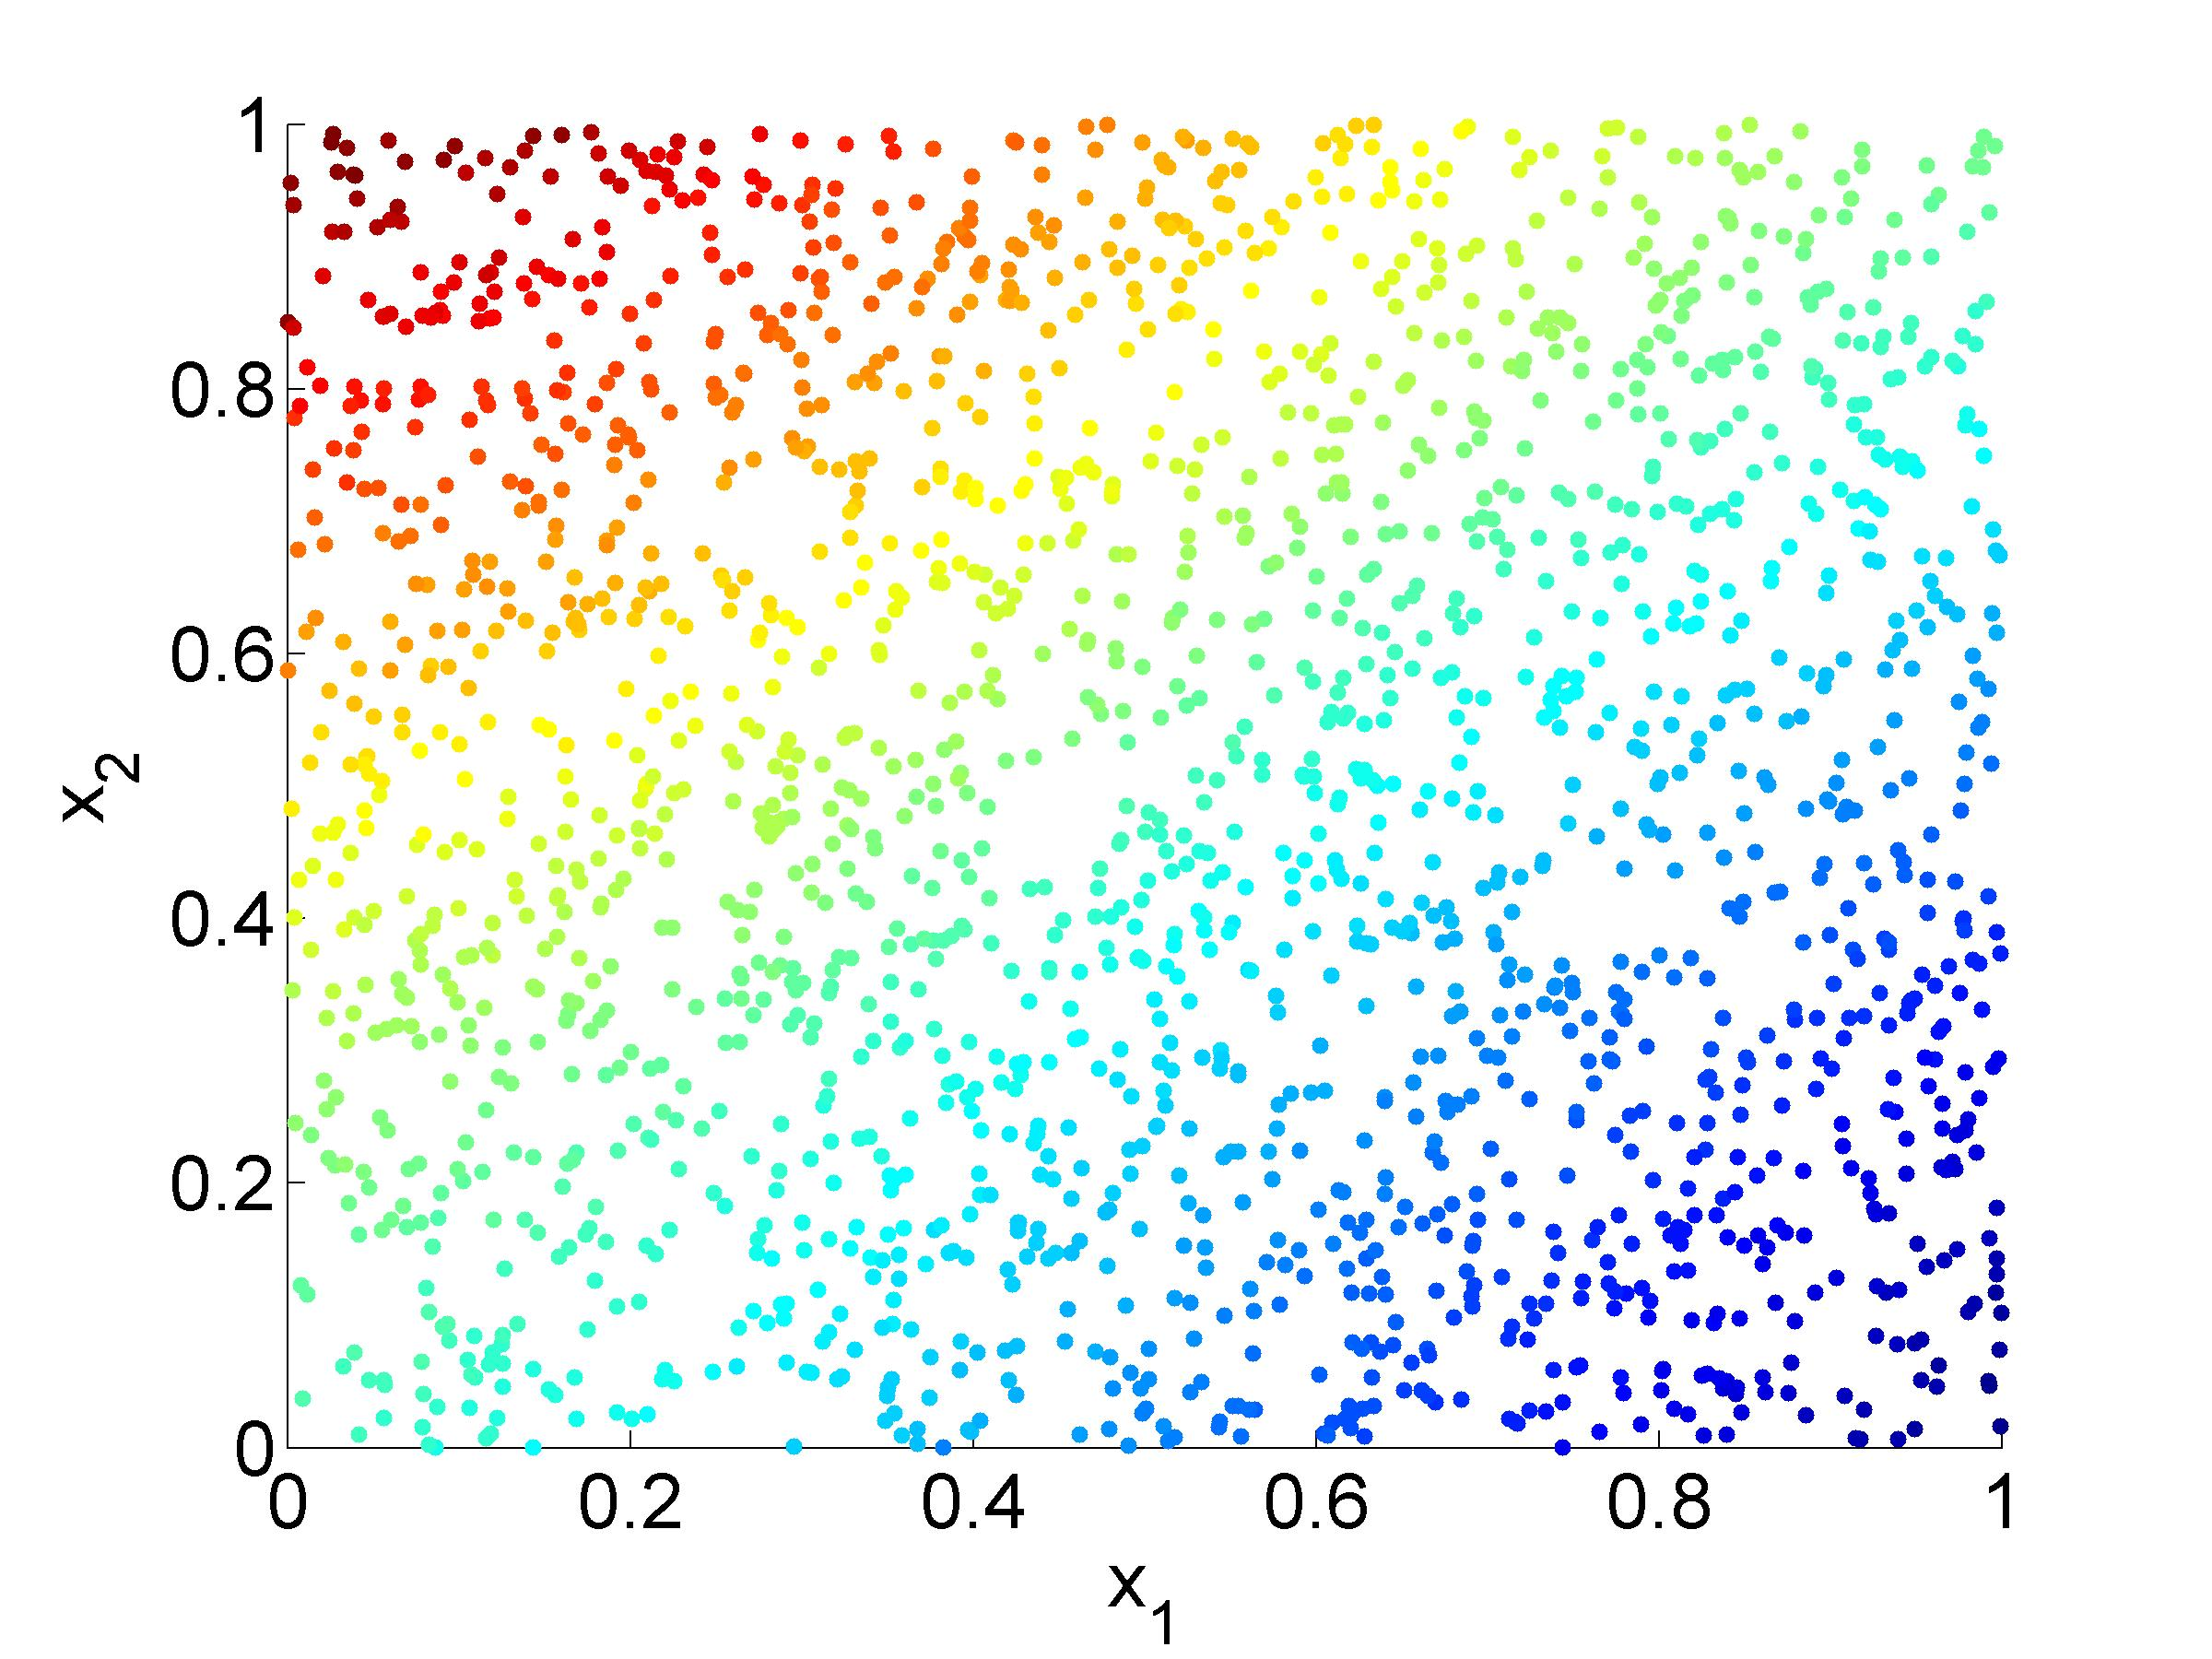
\includegraphics[width=0.3\textwidth]{xdata_noise1_colored_NIV1}
%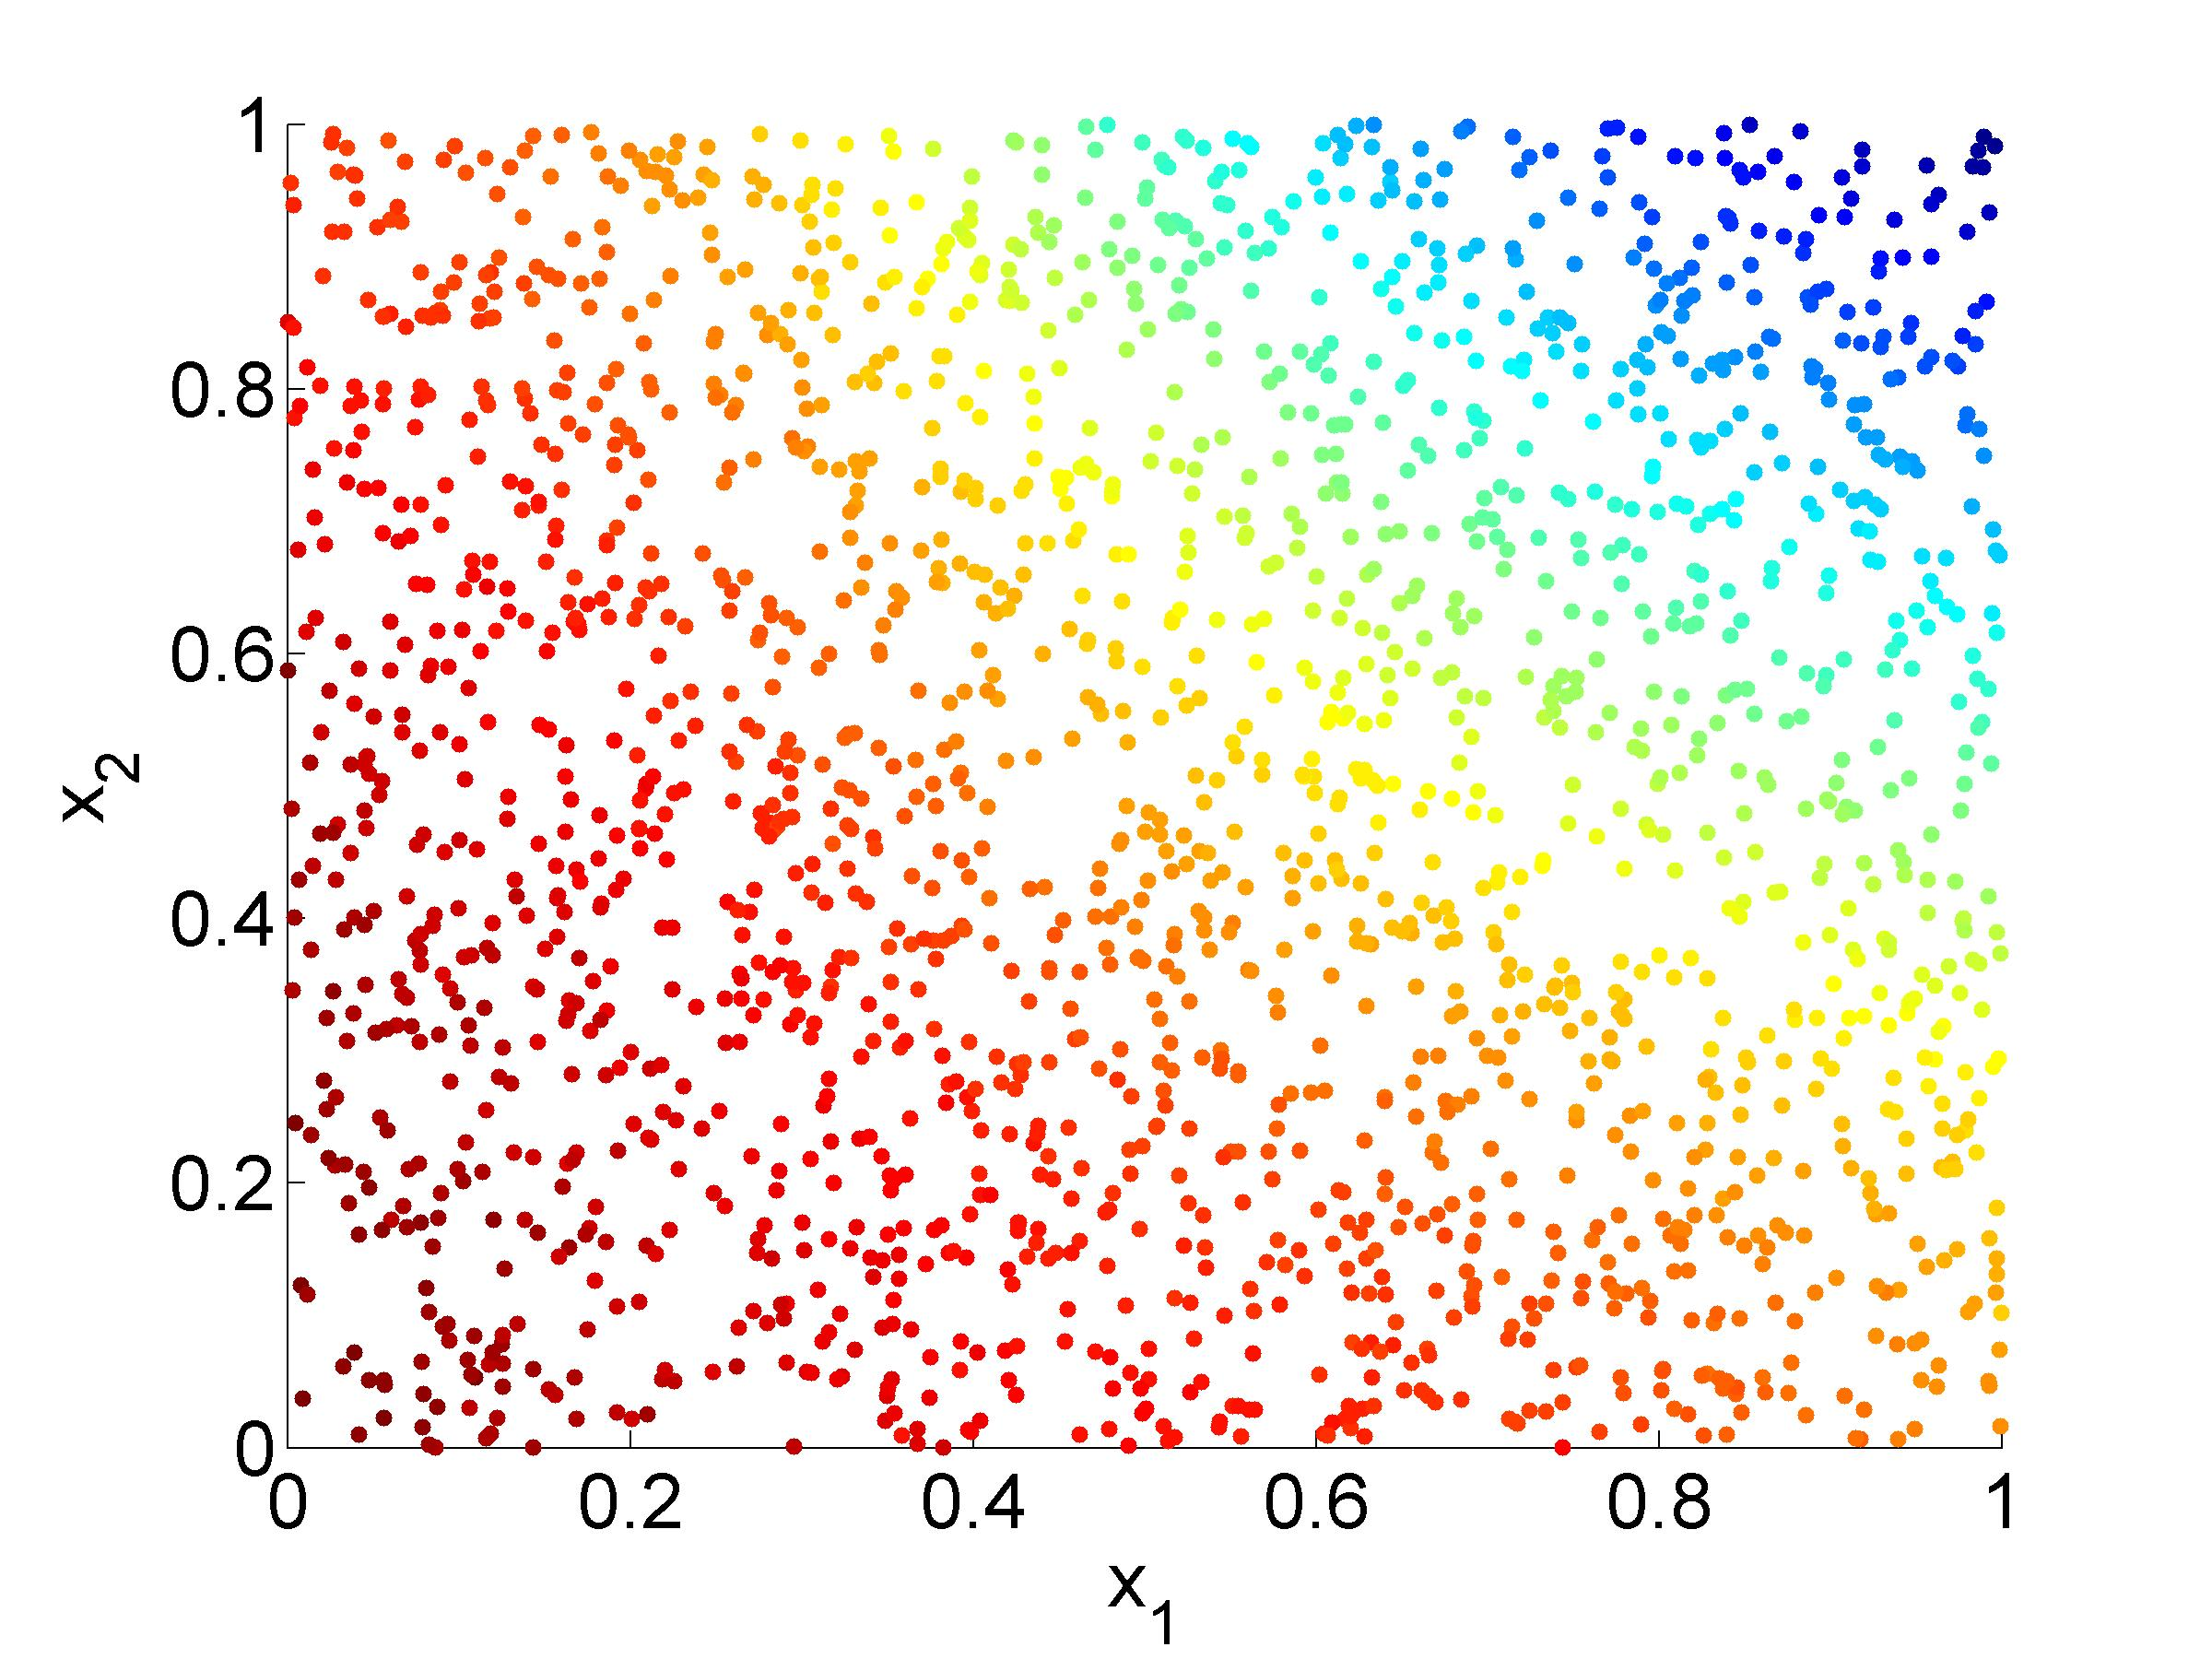
\includegraphics[width=0.3\textwidth]{xdata_noise1_colored_NIV2}
%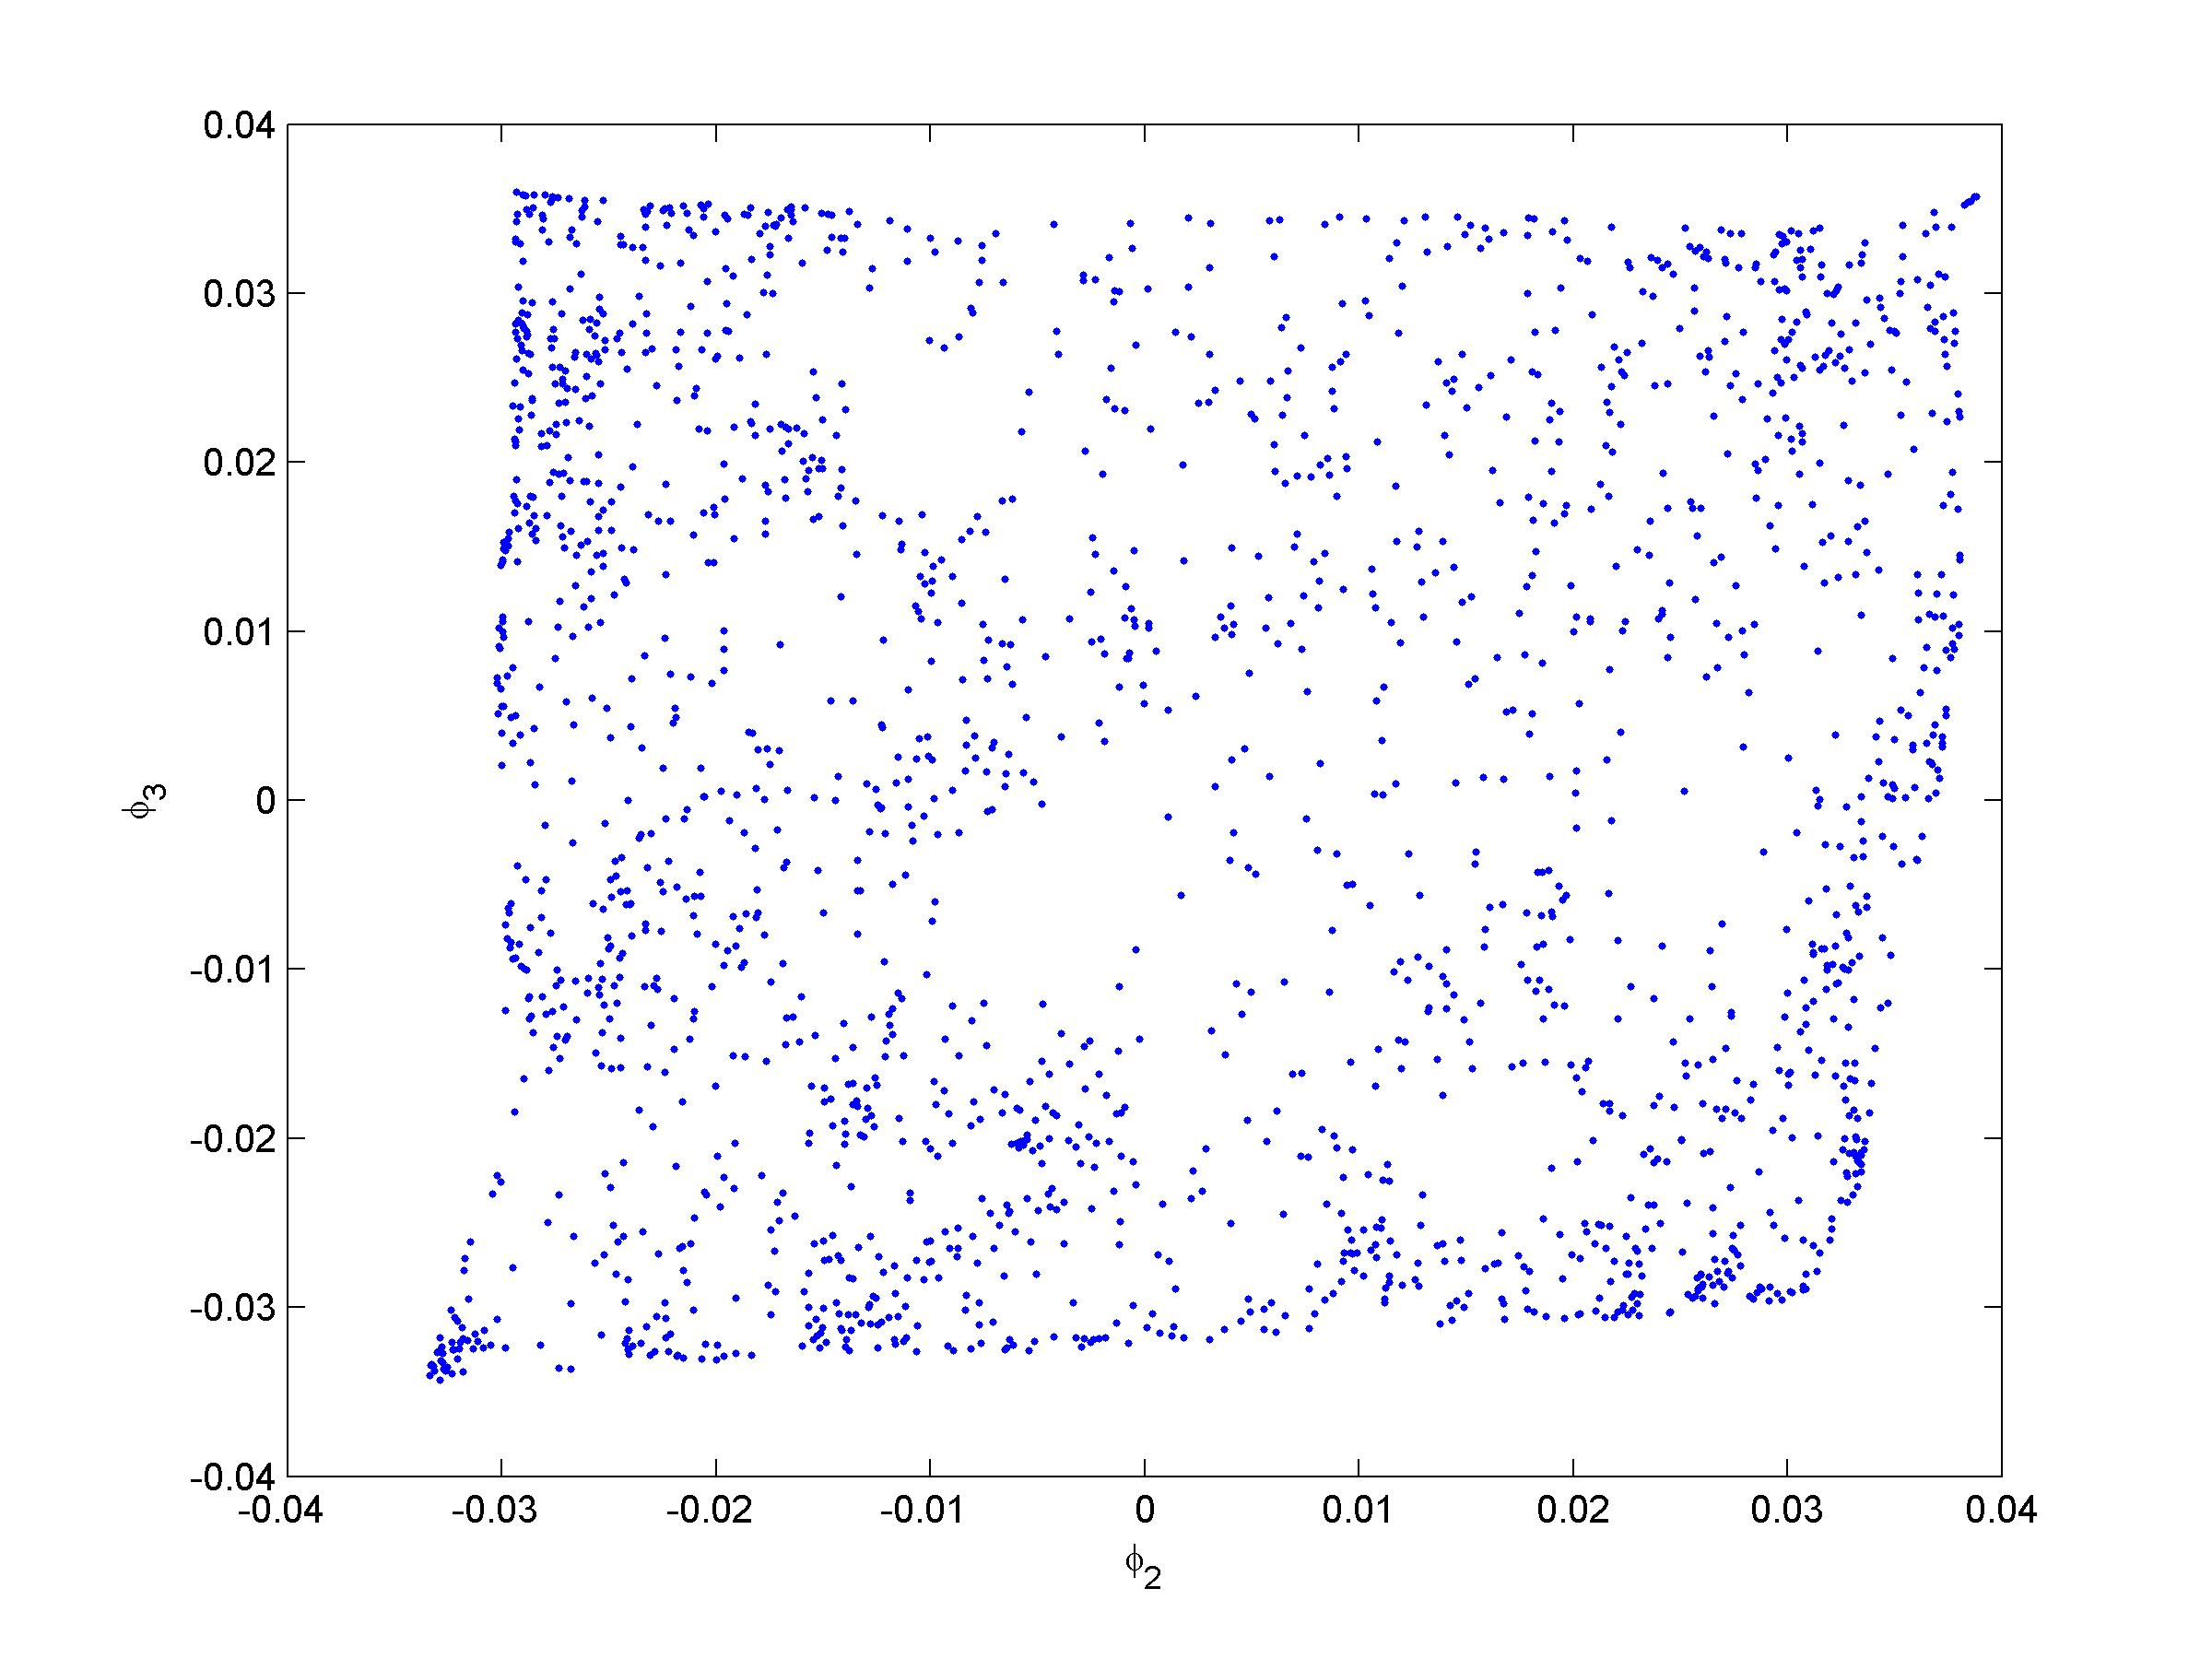
\includegraphics[width=0.3\textwidth]{embedding_noise1}
%\caption{Data in ``intrinsic variable'' space ($x_1, x_2$), colored by the first (left) and second (center) nontrivial NIV. The NIV embedding is computed from the data in the ambient space with added noise ($z_1, z_2$, with $\sigma = 0.01$). Note that the parameterizations we obtain are the eigenfunctions that we expect for points sampled from the unit square. (right) Data plotted in first two (nontrivial) NIV. We (effectively) recover the unit square, i.e., the domain of the intrinsic variables. }
%\label{fig:xdata_NIV_noise1}
%\end{figure}
%
%If $\sigma = 100$ (so the added noise is much larger than the noise in the original clouds), we obtain a parameterization shown in Figure \ref{fig:xdata_NIV_noise2} using NIV.
%%
%Now, the ellipses are a combination of the intrinsic variable noise and the ambient space noise, but the ambient space noise is {\em much} larger. 
%%
%Therefore, NIV only collapses the ambient space noise (not the intrinsic variable noise), and so we get something like the DMAPS coordinates, rather than the NIV. 
%
%\begin{figure}[H]
%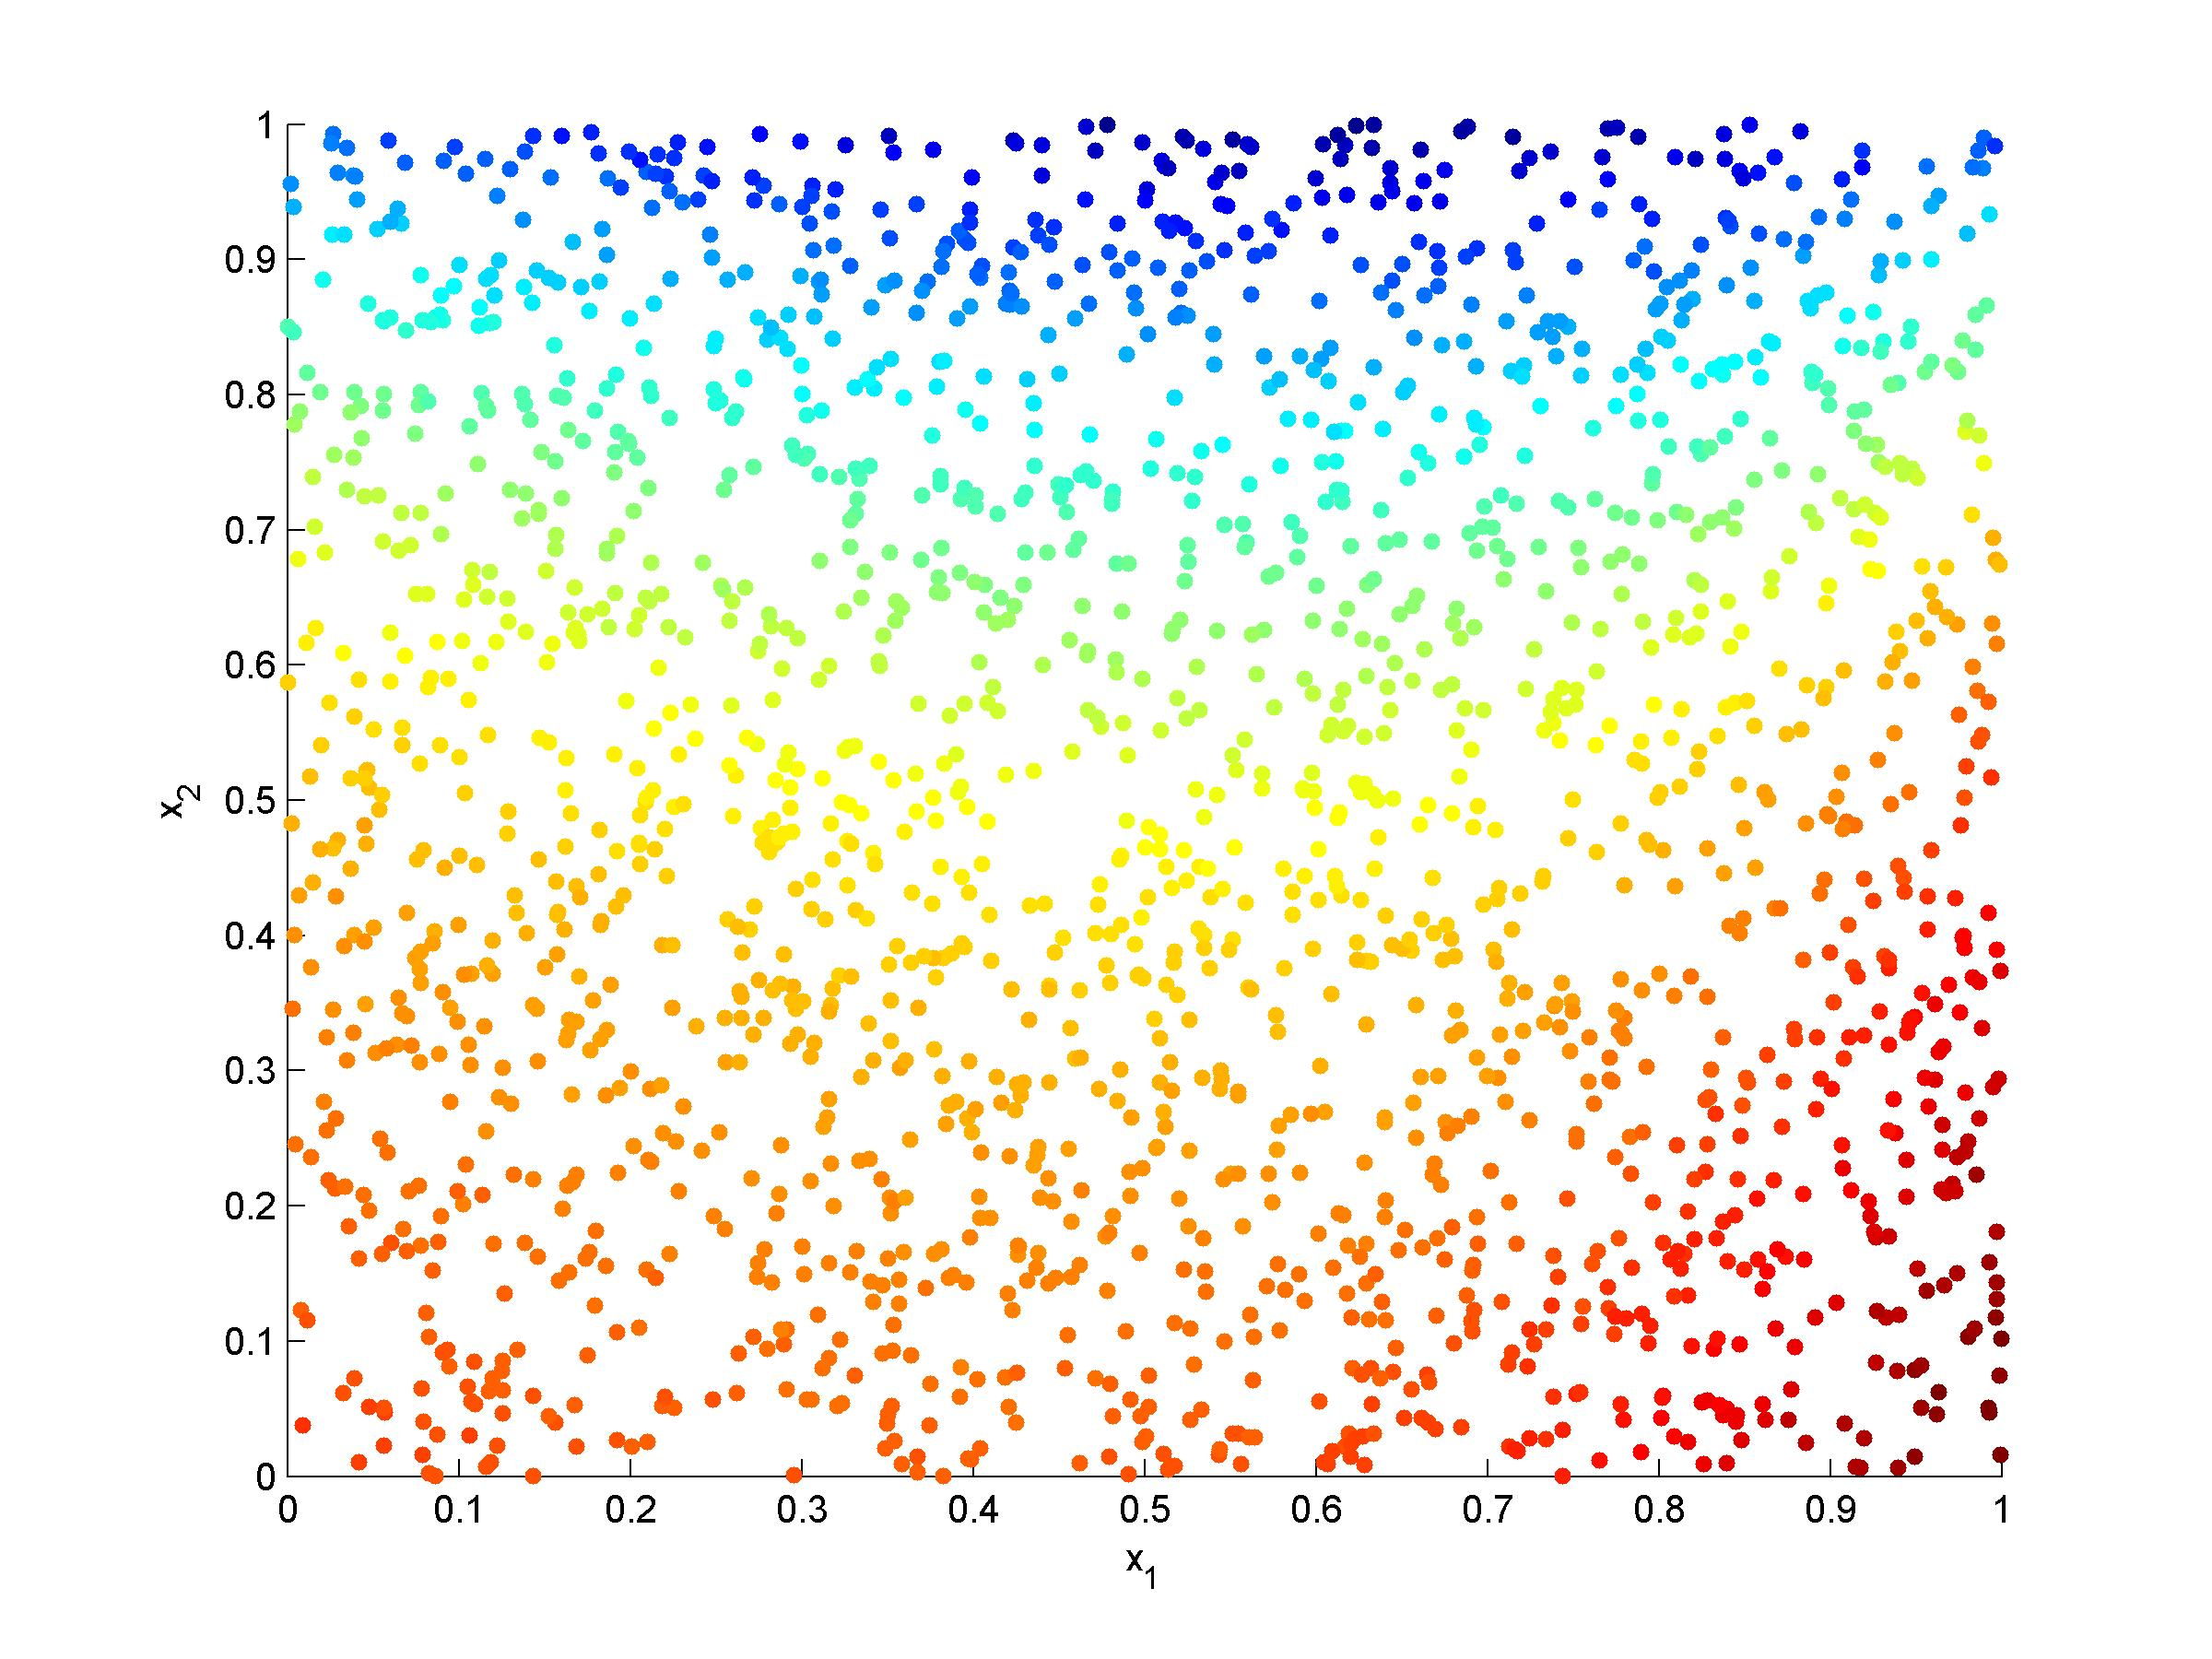
\includegraphics[width=0.3\textwidth]{xdata_noise2_colored_NIV1}
%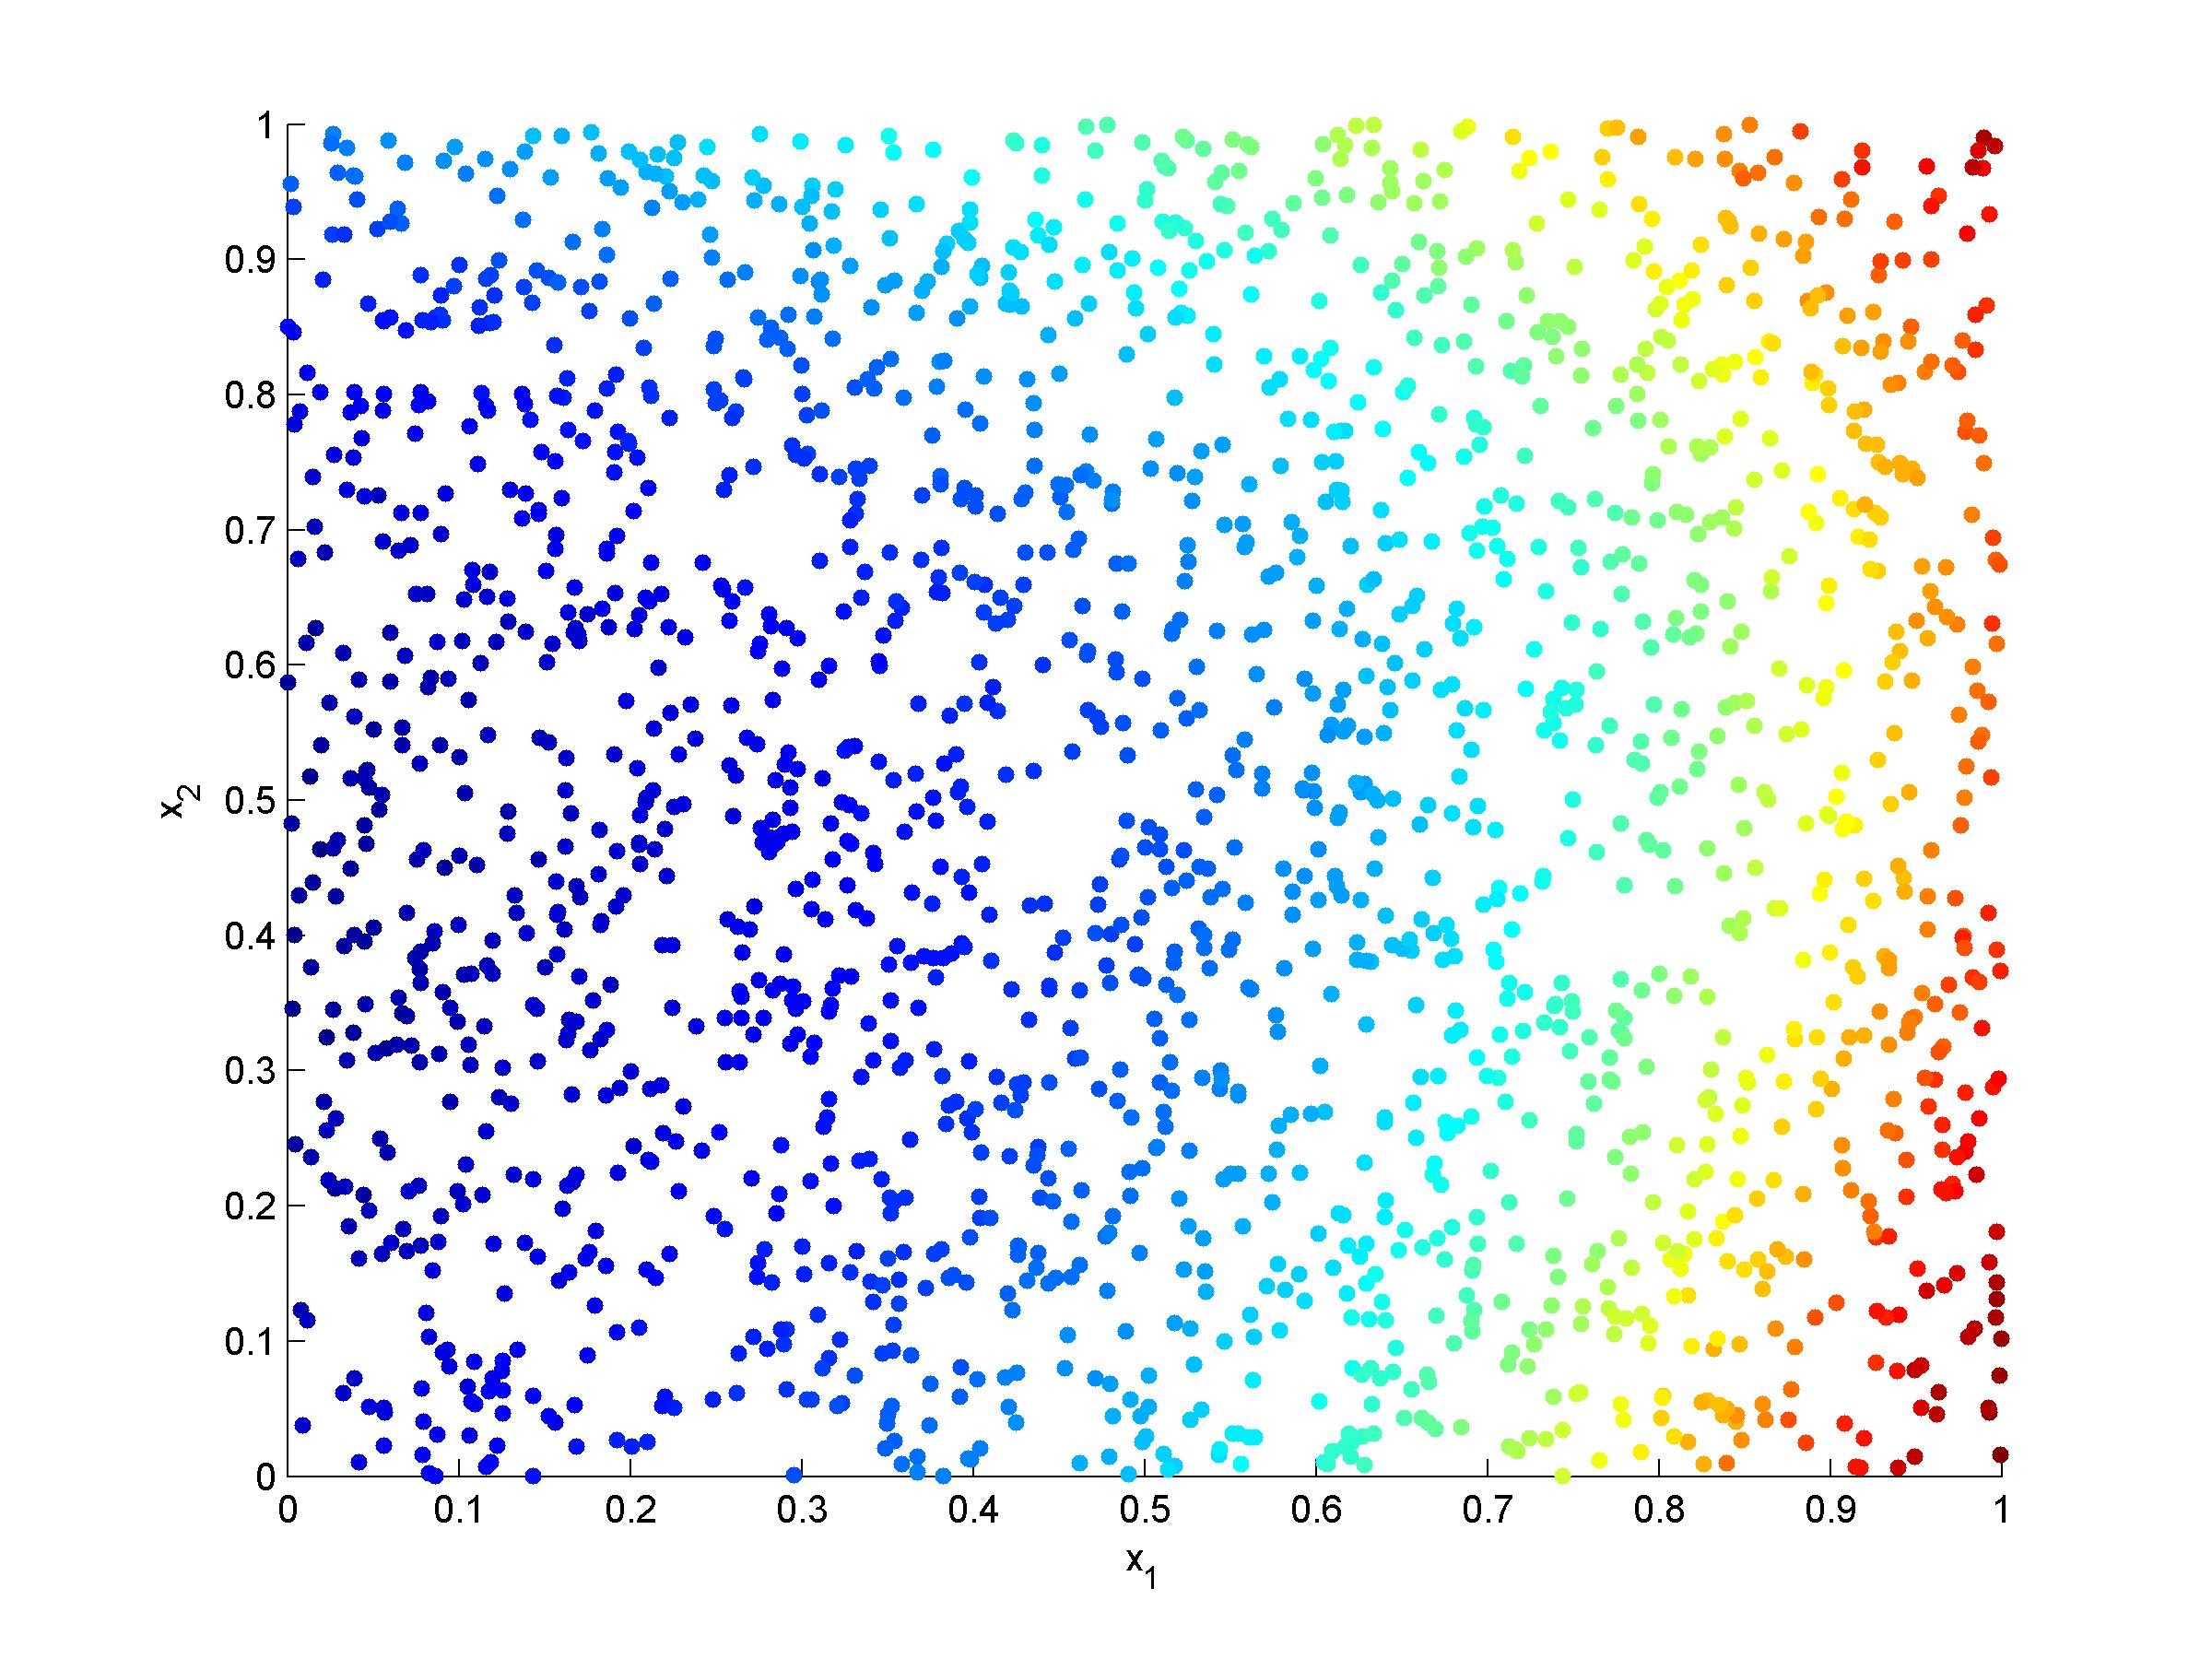
\includegraphics[width=0.3\textwidth]{xdata_noise2_colored_NIV2}
%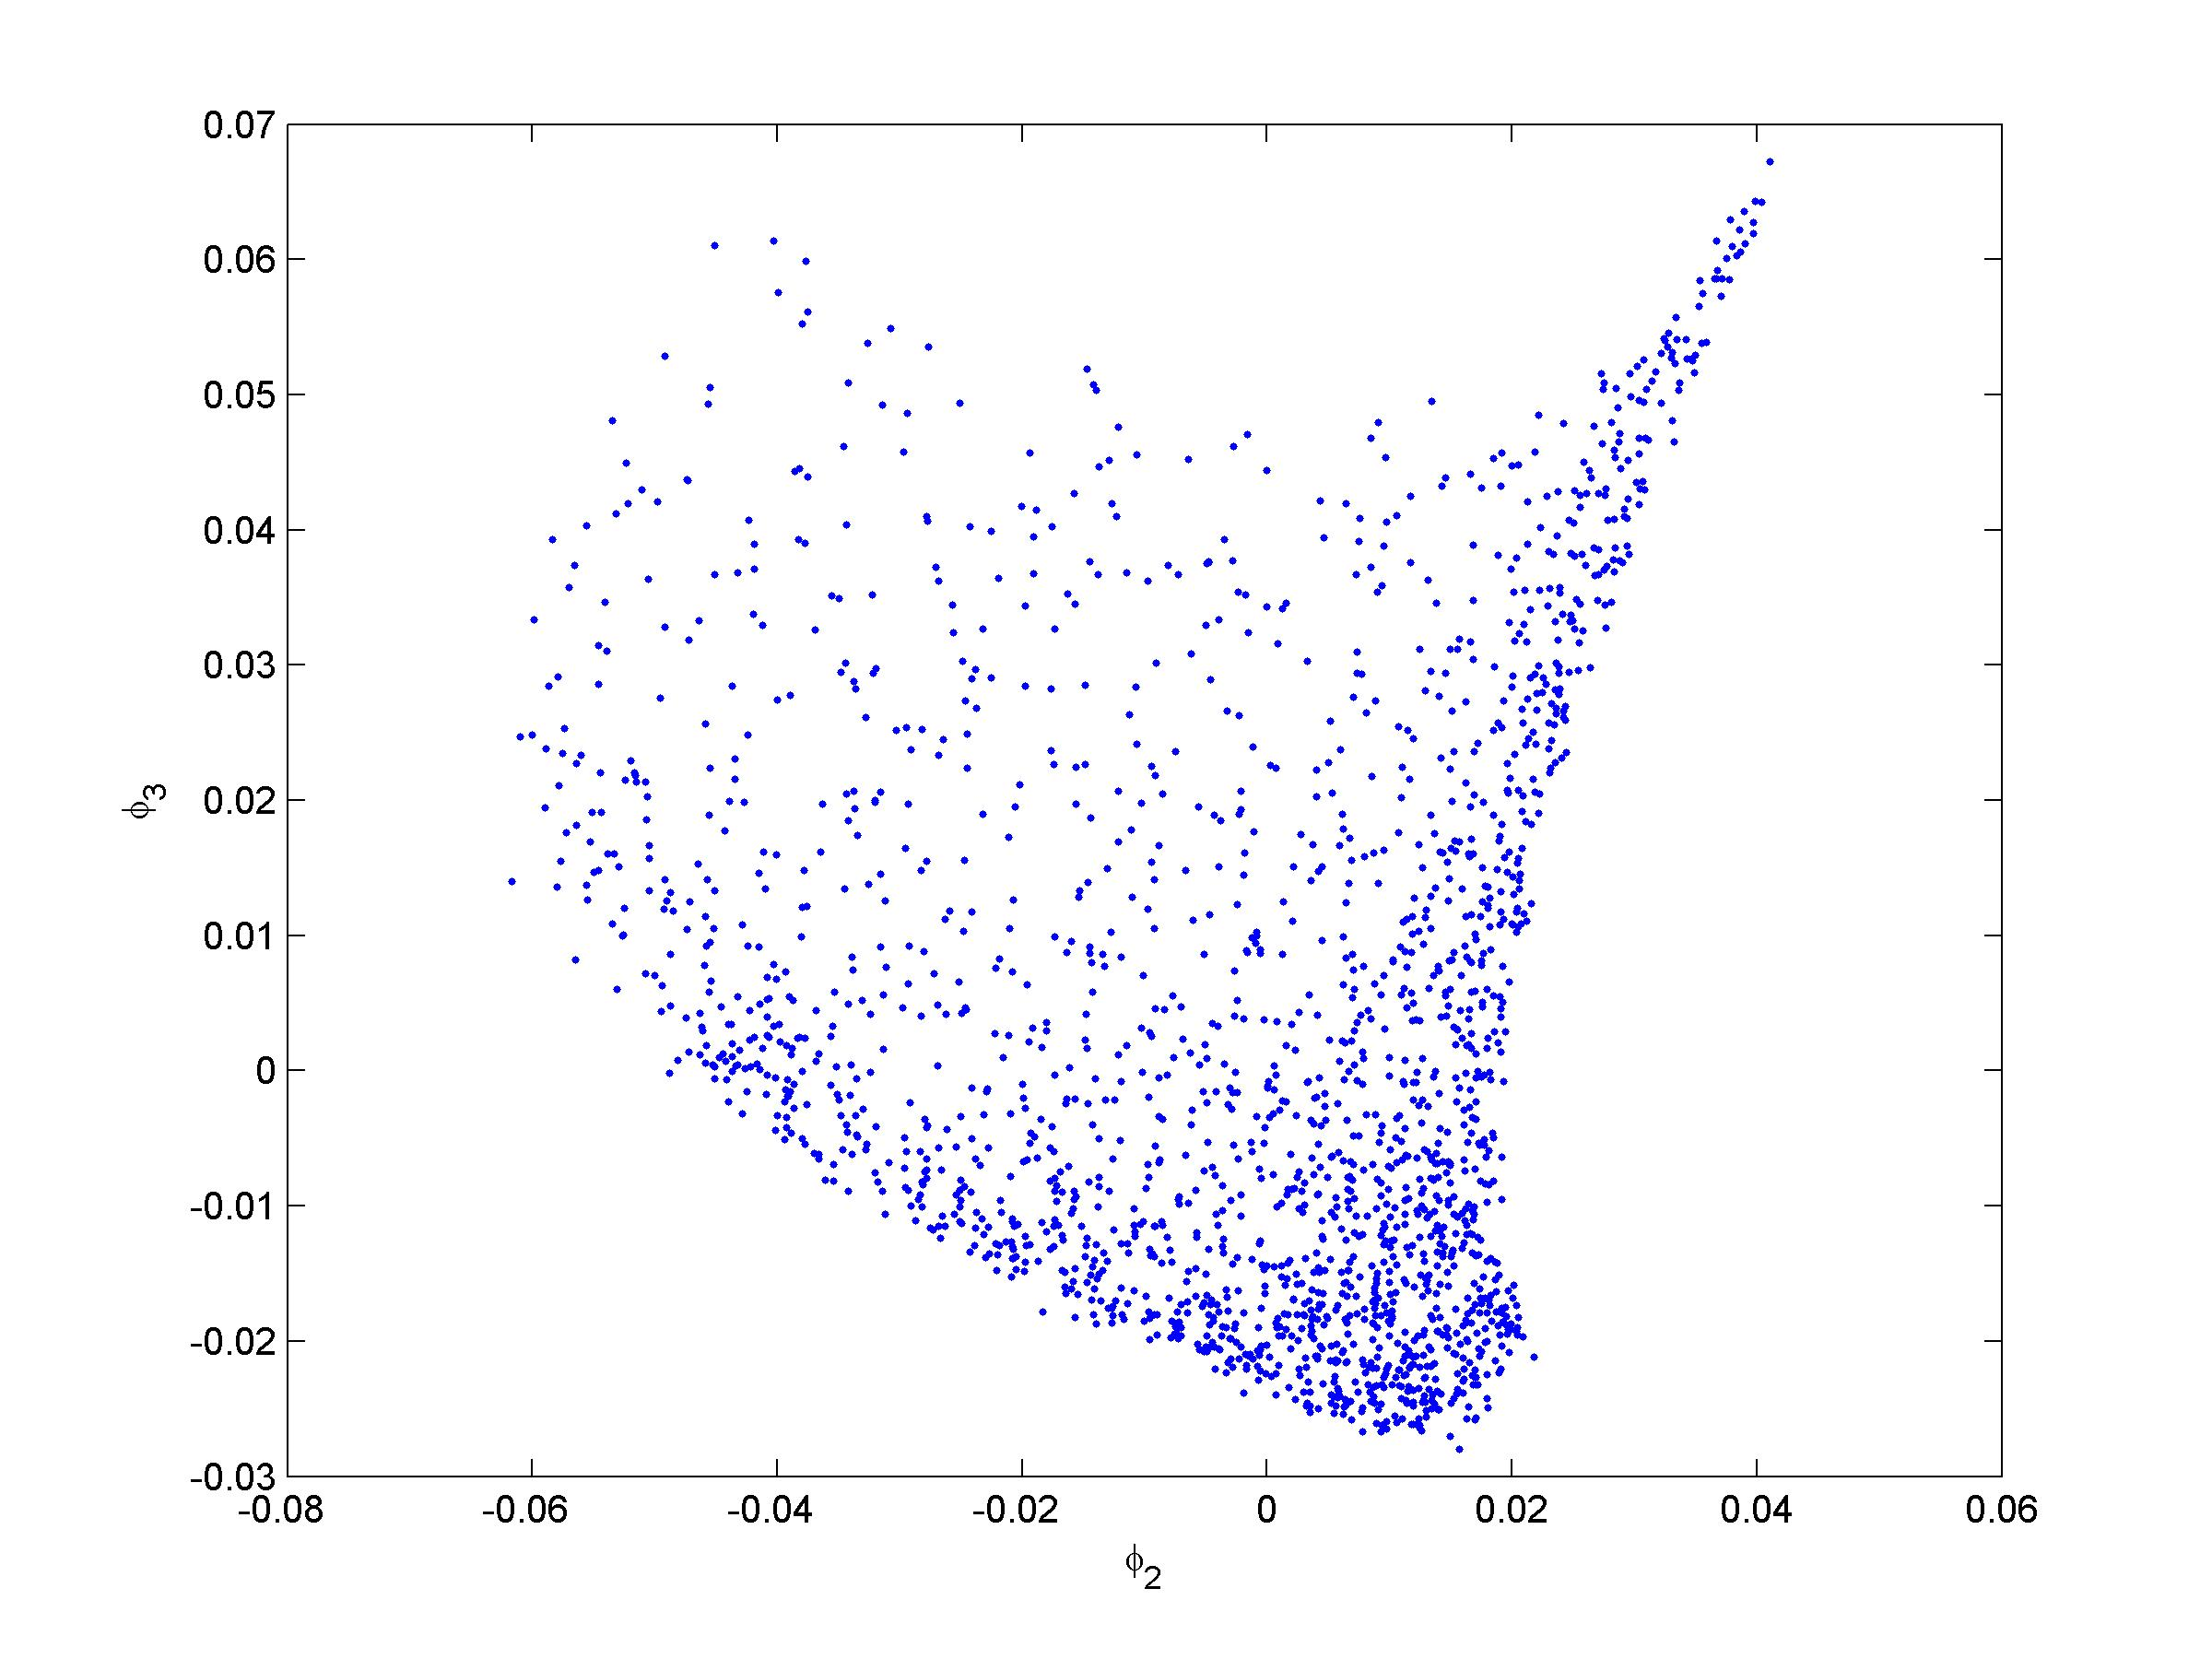
\includegraphics[width=0.3\textwidth]{embedding_noise2}
%\caption{Data in ``intrinsic variable'' space ($x_1, x_2$), colored by the first (left) and second (center) nontrivial NIV. The NIV embedding is computed from the data in the ambient space with added noise ($z_1, z_2$, with $\sigma = 100$). Note that the parameterizations we obtain are not the eigenfunctions that we expect for points sampled from the unit square, but are now similar to the parameterizations obtained from DMAPS shown in Figure \ref{fig:xdata_dmaps}. (right) Data plotted in first two (nontrivial) NIV. We do {\em not} recover the unit square.}
%\label{fig:xdata_NIV_noise2}
%\end{figure}

\section{Analysis using Stochastic Calculus}

We will use the model described in \eqref{eq:NIV_model}, where $\theta$ are our intrinsic variables, and our observations will be $x = f(\theta) + \xi$.  
%
We assume that the timescale of the noise $\xi$ is faster than the timescale of the intrinsic variables $\theta$. 

%We have a 2-scale problem (assuming $s_2 > s_1$). This problem can be extended to multiscale problems naturally. 

%The problem: the NLICA analysis is based on the following linearization of the measurement function (for simplicity around $\theta = 0$):
%\[
%	x_t = \nabla f \theta _t + \frac{1}{2} \theta_t ^T \nabla ^2 f \theta_t + \epsilon _t
%\]
%and assume $\epsilon _t$ is small.

Applying the Ito lemma gives us
\begin{equation}
dx_t^j =  \sum_{i=1}^d \left( \frac{1}{2}  \frac{\partial ^2 f^j}{\partial \theta_i^2} + a_t^i \frac{\partial f^j}{\partial \theta_i} \right) dt + \sum_{i=1}^{d} \frac{\partial f^j}{\partial \theta_i} dW_t^i + d \xi_i(t)
\end{equation}

Assuming that the derivatives are constant in the time interval $\delta t$,
\begin{eqnarray}
\hat{\mu}_t^j = \frac{1}{\delta t} \int_{t}^{t + \delta t} dx_t^j &=& 
\frac{1}{\delta t} \int_{t}^{t + \delta t} \sum_{i=1}^d \left( \frac{1}{2}  \frac{\partial ^2 f^j}{\partial \theta_i^2} + a_t^i \frac{\partial f^j}{\partial \theta_i} \right) dt + \sum_{i=1}^{d} \frac{\partial f^j}{\partial \theta_i} dW_t^i + \frac{1}{\epsilon} d \hat{W}^j_t \\
&=& \frac{1}{\delta t} \sum_{i=1}^d \left( \frac{1}{2}  \frac{\partial ^2 f^j}{\partial \theta_i^2} + a_t^i \frac{\partial f^j}{\partial \theta_i} \right) \delta t + \frac{1}{\delta t} \sum_{i=1}^{d} \frac{\partial f^j}{\partial \theta_i} V_i + \frac{1}{\delta t \epsilon} V_{d+1}\\ 
&=& \sum_{i=1}^d \left( \frac{1}{2}  \frac{\partial ^2 f^j}{\partial \theta_i^2} + a_t^i \frac{\partial f^j}{\partial \theta_i} \right) + \mathcal{N}\left( 0, \frac{1}{\delta t} \sum_{i=1}^d \left( \frac{\partial f^j}{\partial \theta_i} \right)^2 + \frac{1}{\delta t \epsilon^2} \right)\\
&=& \sum_{i=1}^d \left( \frac{1}{2}  \frac{\partial ^2 f^j}{\partial \theta_i^2} + a_t^i \frac{\partial f^j}{\partial \theta_i} \right) + U^j
\end{eqnarray}
where $V_i \sim \mathcal{N}(0, \delta t)$ and $U^j \sim \mathcal{N}\left( 0, \frac{1}{\delta t} \sum_{i=1}^d \left( \frac{\partial f^j}{\partial \theta_i} \right)^2 + \frac{1}{\delta t \epsilon^2} \right)$.


\begin{eqnarray}
dx_t^j dx_t^k &=& 
\left( \sum_{i=1}^d \left( \frac{1}{2}  \frac{\partial ^2 f^j}{\partial \theta_i^2} + a_t^i \frac{\partial f^j}{\partial \theta_i} \right) dt + \sum_{i=1}^{d} \frac{\partial f^j}{\partial \theta_i} dW_t^i + \frac{1}{\epsilon} d \hat{W}^j_t \right) \\
&& \left( \sum_{i=1}^d \left( \frac{1}{2}  \frac{\partial ^2 f^k}{\partial \theta_i^2} + a_t^i \frac{\partial f^k}{\partial \theta_i} \right) dt + \sum_{i=1}^{d} \frac{\partial f^k}{\partial \theta_i} dW_t^i + \frac{1}{\epsilon} d \hat{W}^k_t \right) \\
&=& \sum_{i=1}^d \frac{\partial f^j}{\partial \theta_i} \frac{\partial f^k}{\partial \theta_i} dW_t^i dW_t^i + \frac{\delta_{jk}}{\epsilon^2}  d \hat{W}^j_t d \hat{W}^k_t  \\
&=& \sum_{i=1}^d \frac{\partial f^j}{\partial \theta_i} \frac{\partial f^k}{\partial \theta_i} dt + \frac{\delta_{jk}}{\epsilon^2}  d t
\end{eqnarray}

\begin{eqnarray}
\frac{1}{\delta t} \int_{t}^{t + \delta t} dx_t^j dx_t^k &=& \frac{1}{\delta t} \int_{t}^{t + \delta t} \sum_{i=1}^d \frac{\partial f^j}{\partial \theta_i} \frac{\partial f^k}{\partial \theta_i} dt + \frac{\delta_{jk}}{\epsilon^2}  d t  \\
&=& \sum_{i=1}^d \frac{\partial f^j}{\partial \theta_i} \frac{\partial f^k}{\partial \theta_i}+ \frac{\delta_{jk}}{\epsilon^2}
\end{eqnarray}


\begin{eqnarray}
\hat{C}_t^{jk} &=& \frac{1}{\delta t} \int_{t}^{t + \delta t} dx_t^j dx_t^k -  \hat{\mu}_t^j \hat{\mu}_t^k \\
&=& \sum_{i=1}^d \frac{\partial f^j}{\partial \theta_i} \frac{\partial f^k}{\partial \theta_i}+ \frac{\delta_{jk}}{\epsilon^2} - \\
&& \left(\sum_{i=1}^d \left( \frac{1}{2}  \frac{\partial ^2 f^j}{\partial \theta_i^2} + a_t^i \frac{\partial f^j}{\partial \theta_i} \right) + U^j \right) \left(\sum_{i=1}^d \left( \frac{1}{2}  \frac{\partial ^2 f^k}{\partial \theta_i^2} + a_t^i \frac{\partial f^k}{\partial \theta_i} \right) + U^k \right)
\end{eqnarray}


Define 
\begin{equation}
J = \left[ \frac{\partial f^j}{\partial \theta_i} \right]_{ji}
\end{equation}

\begin{equation}
H = \left[ \frac{\partial^2 f^j}{\partial \theta_i^2} \right]_{ji}
\end{equation}

Then
\begin{eqnarray}
\hat{C}_t &=& J J^T + \frac{1}{\epsilon^2} I - \left( \frac{1}{2} H \mathbf{1} + J a + U \right) \left ( \frac{1}{2} H \mathbf{1} + J a + U \right)^T \\
&=& J J^T + \frac{1}{\epsilon^2} I - \left[ \frac{1}{4} H \mathbf{1} \mathbf{1}^T H^T + J a a^T J^T + U U^T \right. \\
&+& \left. U \left ( \frac{1}{2} H \mathbf{1} + J a  \right)^T + \left( \frac{1}{2} H \mathbf{1} + J a \right) U^T  + \frac{1}{2} H \mathbf{1} a^T J^T + \frac{1}{2} J a \mathbf{1}^T H^T \right]
\end{eqnarray}

TODO: fix the above analysis (1) make sure that the calculus is right, (2) are we calculating the covariance of the differences? (3) verify/figure out why the trends are not what we expect (dependency on curvature, drift, scale of noise, $\delta t$, etc.)

For NLICA to work properly, we need to define clouds of points that respect the shape of the distortion of $f$ applied to the low dimensional Gaussian of $O(1)$ in the NIVs domain. Obviously, we cannot take clouds with scales smaller than $1/\epsilon$, because then we only see the Gaussian in the ambient domain. Thus, we must take larger scales. On the other hand, large scales could include the intrinsic drift (and possibly the nonlinear parts of the measurement function), and therefore, we would want to take a small as possible scale (but greater than $1/\epsilon$). 
%Consider the smallest possible choice -- clouds of scale $s_2$ and observe:
%\begin{eqnarray}
%	x_{t+s_2} &=&  \nabla f \theta _{t+s_2} + \frac{1}{2} \theta_{t+s_2} ^T \nabla ^2 f \theta_{t+s_2} \\
%	&=& \nabla f (\theta _t + s_2 a _t + s_2 s_1 \tilde{\xi}) \\
%	&+& \frac{1}{2} (\theta _t + s_2 a _t + s_2 s_1 \tilde{\xi}) ^T \nabla ^2 f (\theta _t + s_2 a _t + s_2 s_1 \tilde{\xi}), \ \tilde{\xi} \sim \mathcal{N}(0,I)
%\end{eqnarray}
%TODO: replace the last equation with the ito lemma application from the NLICA paper (eq. (4)). Then, fix the following, and also make it scalar (one coordinate of $x_t$).
%The empirical mean is (for each coordinate):
%\begin{eqnarray}
%	\hat{\mu}_t &=& \frac{1}{N} \int \limits _{t+\tau, \tau \in [-s_2,s_2]} x_{t+\tau}, \ \ N = |[-s_2,s_2]| \\
%		&=& \frac{1}{N} \int \limits _{t+\tau, \tau \in [-s_2,s_2]} ( \nabla f \theta _{t} + \frac{1}{2} \theta_{t} ^T \nabla ^2 f \theta_{t}) \\
%		&+& \frac{1}{N} \int \limits _{t+\tau, \tau \in [-s_2,s_2]}  (\nabla f(0) \tau a _t + \tau^2 a_t^T \nabla ^2 f a_t ) \\
%		&+& \frac{1}{N} \int \limits _{t+\tau, \tau \in [-s_2,s_2]}  (\nabla f(0) \tau s_1 \tilde{\xi} + \tau^2 s_1^2 \tilde{\xi}^T \nabla ^2 f \tilde{\xi}) \\
%		&=& x_t + a_t^T \nabla ^2 f a_t \frac{2 s_2^3}{3} + s_1^2 \mathrm{tr} (\nabla ^2 f) \frac{2 s_2 ^3} {3}
%\end{eqnarray}
%We need to repeat that for the empirical covariance. However, at this point we can observe that: (1) the intrinsic drift, the intrinsic scale, the Hessian of the measurement function, and the chosen/fast scale, play a role and distort the cloud. (2) In order for NLICA to work (again, we need to verify for the covariance and write with the all the details) we require that $1 / s_2 ^3 \sim \nabla^2 f s_1^2, \nabla^2 f a_t^2$.

In conclusion, given a problem in which these conditions/relations between the scales and the measurement function and the drift do not hold, we cannot recover NIVs from the measurements in a single application of NLICA/Mahalanobis graph.

\section{Intermediate Variables and Iterative Algorithm}

Basically, in the ambient space, we get such clouds of data:
\[
	e^{-z^T(C_y(t) + C_\xi(t))^{-1} z}
\]
where $C_y(t)$ is the covariance of the intrinsic noise translated into the ambient space (including the ``curvature" of the nonlinear measurement function), and $C_\xi(t)$ is the covariance of the ambient noise.
%
The point is, for small $t$ ($t < 1/\epsilon$), the size of the ambient noise could be much larger than the intrinsic noise (and thereofre, $C_\xi \gg C_y$). 
%
In this regime, we would not get good estimates of $C_y$, which means we will not see the intrinsic noise or recover NIV.
%
However, if we take a larger $t$ ($t > 1/\epsilon$), we may begin to see the curvature of the measurement function, and therefore cannot obtain good estimates of the {\em local} covariance $C_y$. 

The signal $y$ is corrupted with noise $\xi$.
%
We assume that the noise is faster than the signal. 
%
We also assume that the noise saturates/have a fixed length scale.
%
We use these two assumptions to separate between the signal and the noise by averaging/computing expected values and slowing down the time scale of the measurements.

Since the measurements of the system are high--dimensional, we cannot compute accurate expected values using the (relatively) small number of samples.
%
So, we first project the data into a lower--dimensional space, where the averaging will be more robust/efficient/better.
%

For example, we could project the data onto random ``histogram'' boxes such that the projected data in those boxes such that the intrinsic noise is fixed, and we see only the ambient noise (and the ambient noise has saturated).
%
We would then use the projections as our new measurments/observations, and recover their NIVs, which would be (by definition) the NIVs of the original (slow) data. 

An empirical way to do it: 1. Choose random boxes. 2. pick the time scale according to Mauro's method - (local PCA of the boxes) - start with a large scale (again, when the data is restricted to the low d boxes), and then start decreasing the scale, until we get a fixed number of dimensions with a fixed spectrum. At large scales - the spectrum would ``see" the shape of the manifold (depending on the curvature of the nonlinear measurement function embedded/restricted in the box) and at smaller scales, the restriction of the manifold to the box will be flat and then we would see just the restricted ambient noise (giving a fixed spectrum). All we need to do is to choose enough boxes, in different scales, such that in just few, the description above would hold.

Note: we could also do this by starting with a small time scale, and then increasing until we see the saturation of the fast process/fast noise. 
%
However, this requires us to have a sufficient number of samples to accurately estimate the covariance at this small time scale. 


\subsection{Algorithm}

Input: $x_t$.

\begin{enumerate}
	
	\item
	Draw filters $\psi _k$, k = 1, \ldots, K.
	
	\item
	\label{algo:iter_begin}
	Pick (and peal) the ``finest time scale":
	
	Pick a large scale $\delta t$, aiming for a scale $\delta t > 1/\epsilon$.
		
		
	BEGIN WHILE $\| C_j - C_{j-1} \| > thr$

	\begin{enumerate}
		\item
		Ideally, if $\delta t < 1/\epsilon$, then NLICA failed and we probably need better observables. In practice, $1/\epsilon$ is unknown, and therefore, we take enough random observables such that at least few will be good.
		
		\item
		Project the data onto $\psi _k$ and get the ``random projections": $o_{t,k} = \langle x_t, \psi _k \rangle$.
		
		\item
		Compute the (empirical) covariance $C_j$ of $o_{t,k}$ in a time window of size $\delta t$. This is the variance+bias of the estimator of $\mathbb{E}[o_{t,k}]$ in this window of scale $\delta t$.
			
		\item
		Decrease $\delta t$.
		
	\end{enumerate}	
	END WHILE
	
	Note: instead of looking for convergence of $C$, we could look for convergence of the eigenvalues of $C$ to examine when $C$ is (approximately) an $n$-dimensional Gaussian. 
	
	Explanation: Note, clouds of $x$ samples with scale $1/\epsilon$ see the ambient noise more than the intrinsic noise (after $1/\epsilon$ time units, the ambient noise is saturated, BUT we might begin to see the intrinsic drift or curvature of $f$. This is the reason why NLICA fails.). 
	%
Our goal is to find the timescale at which the fast noise is saturated (so that different clouds only change due to effects from the slow/intrinsic process). 
%
When the fast noise has saturated, changing the timescale $\delta t$ of the clouds should not (significantly) change the covariance of the clouds (this is the termination condition for our algorithm). 

We start with a large scale ($\delta t > 1/\epsilon$). 
%
The goal of this step in the algorithm is to find $1/\epsilon$, the saturation time of the fast noise.
%
We assume that, when $\delta t > 1/\epsilon$, the clouds/covariances will see the drift of the intrinsic variables and the curvature of the measurment function, and so the covariance will change from iteration to iteration.
%
When our assumptions hold within the timescale $\delta t$ (there is little drift and the measurement function is relatively flat), and when the fast noise $\xi$ is saturated, the covariances should not change significantly from iteration to iteration. 
 %If at any point, we discover the clouds of our new observables $o_{t,k}$ with scale smaller or equal $s_2$ still see the intrinsic drift (or curvature), then, these observable are not useful. 
 %In practice, $s_2$ is unknown and therefore we cannot check this case. 
% 
 The idea of the iterative procedure is to find the largest possible scale of clouds of observables that does not see the intrinsic drift and the curvature. 
We examine that by searching a cloud that is relatively constant (with respect to the time window) in the dimension of the ambient space. 
%
In practice, this is done by looking at the change in the covariances as we change the time window.
	
	\item
	Compute the estimators of the observables $\hat{o}_{t,k} = \hat{\mathbb{E}}[o_{t,k}]$ in the chosen scale $\delta t^*$ by integrating in windows of this size.
	
     \item
	Apply the Mahalanobis graph to the new observables $\hat{o}_{t,k}$ and examine whether the eigenvectors recover NIVs. Note: (1) The observables are at a slower rate than the raw measurements $x$. (2) This step cannot be verified in practice (?) since the NIVs are unknown.

	\item
	If yes -- stop, If no (then, we are dealing with the case described above - conditions are not met) -- proceed
	
	\item
	Assign $\hat{o}_{t,k} \mapsto x$ and jump to step \ref{algo:iter_begin}.
	
\end{enumerate}

TODO: implement algorithm, verify that it works

\subsection{Histograms}

Just a connection to previous work. Note:
\begin{itemize}
	
	\item
	The above procedure does not generalize the introduction of histograms as intermediate observables. For histograms, we need to replace (or generalize) the linear project onto $\psi_k$ by
	\[
		\hat{o}_{t,k} = \int \langle x _t , \psi _k \rangle p(x) dx \mapsto \int \psi_k( x _t) p(x) dx
	\]
	Then, by setting $\psi _k (x) = \mathbf{1}_{b_k} (x) $, where $b_k$ is some histogram bin (box) in the ambient space, we get
	\[
		\hat{o}_{t,k} = \int \mathbf{1} _{b_k} ( x _t) p(x) dx = \int \limits _{b_k} p(x) dx = \mathcal{L} (p(x))
	\]
	where $\mathcal{L}$ is a linear operator.
	
	\item
	However, the histograms do have a nice property (which we do not loose by replacing it with linear projection onto random vectors, but we do loose it if we generalize and use nonlinear transforms) -- the linearity of ambient noises. For example
	\[
		x_t = f(\theta _t ) + \xi _t = s_t + \xi_t \rightarrow p(x) = p(s)*p(\xi) = \mathcal{L}_{\xi} (p(s))
	\]
	Assuming $\xi$ is stationary (at least locally), we get
	\[
		\hat{o}_{t,k} = \mathcal{L} (p(x)) = \mathcal{L} ( \mathcal{L}_{\xi} (p(s)))
	\]
	Meaning, the observables are linear transformations of the statistics of the signal (and the ambient noise is in the linear transformation). Then, by using the Mahalanobis distance, which is invariant to linear transformations, we get a procedure that is independent of the ambient noise.
	
	\item
	We do not have to use all the histogram bins (i.e., to tile the entire ambient  space) -- all we need is a coverage that ``sees enough". In addition, the ``bins" can be just random directions of any dimension.
	
	 
\end{itemize}





\end{document}